% \documentclass[10pt,final,journal,compsoc,twoside]{IEEEtran}
%\RequirePackage{amsmath}
\documentclass[preprint,11pt]{elsarticle} 
%\smartqed
\usepackage[ruled]{algorithm2e}
%\usepackage{algorithmic}
\usepackage{amssymb}
\usepackage{amsmath}
\usepackage{times,epsfig,proof,url}
\usepackage{epsfig}
\usepackage{epstopdf}
\usepackage{listings}
\usepackage{subfig}
\usepackage{lipsum}
%\usepackage{subfigure}
\usepackage{multicol,multirow}
%\usepackage{algorithm}
\usepackage[noend]{algpseudocode}
\usepackage{textcomp}
\usepackage{color}
%\usepackage[lined,algonl,ruled]{algorithm2e}
% \usepackage{subfigure}
\usepackage{graphicx}
\usepackage[T1]{fontenc}
%\usepackage{subfloat}

\newcommand{\secref}[1]{Section \ref{#1}}
\newcommand{\figref}[1]{Figure \ref{#1}}
\newcommand{\tabref}[1]{Table \ref{#1}}
\newcommand{\equref}[1]{Equation (\ref{#1})}
\renewcommand{\algorithmicrequire}{\textbf{Input:}} 
\renewcommand{\algorithmicensure}{\textbf{Output:}}
%\newcommand{\KZ}[1]{\textcolor{green}{[Kenny: #1]}}
%\newcommand{\JY}[1]{\textcolor{blue}{[Jinyi: #1]}}
\newcommand{\JL}[1]{\textcolor{red}{[Jialing: #1]}}
\newcommand{\KZ}[1]{\textcolor{blue}{[KZ: #1]}}
%\lstset{
%  captionpos=b,
%  tabsize=2,
%  % numbers=left,
%  % numberstyle=\tiny,
%  % numbersep=5pt,
%  breaklines=true,
%  showstringspaces=true,
%  basicstyle=\small,
%  frame=none,
%  emph={label},
%  escapechar=* % Escape to LaTeX between |...|
%}

\renewcommand{\algorithmcfname}{ALGORITHM}
\SetAlFnt{\small}
\SetAlCapFnt{\small}
%\SetAlCapNameFnt{\small}
%\SetAlCapHSkip{0pt}
%\IncMargin{-\parindent}

\begin{document}
% \markboth{IEEE TRANSACTIONS ON KNOWLEDGE AND DATA ENGINEERING}{Lu \textit{et al.}: Fault-Tolerant Optical Character Recognition from Semi-structured Medical Images}
% \markboth{L}{R}
%\markboth{Lu \textit{et al.}{Fault-Tolerant Optical Character Recognition from %Semi-structured Medical Images}
%\markboth{Lu et al.}{Fault-Tolerant Optical Character Recognition from Semi-structured Medical Images}
\begin{frontmatter}

\title{Fault-tolerant Information Extraction from Semi-structured OCR Images
}
% Fault-tolerant Optical Character Recognition
% from Semi-structured Medical Images

% \author
% {Jinyi Lu{\small $^{1}$}, Kenny Q. Zhu{\small $^{2}$}, 
% Weiguo Gao{\small $^{3}$}, Jia Wei{\small $^{4}$} 
% and Meizhuo Zhang{\small $^{5}$}
% \vspace{1.6mm}\\
% \fontsize{10}{10}\selectfont\itshape
% $^{1,2}$ Shanghai Jiao Tong University\\
% $^{3,4,5}$ AstraZeneca China
% \vspace{1.6mm}\\
% \fontsize{9}{9}\selectfont\ttfamily\upshape
% $^{1}$jinyilu93@gmail.com,
% $^{2}$kzhu@cs.sjtu.edu.cn\\
% $^{3,4,5}$\{Weiguo.Gao,Jenny.Wei,Meizhuo.Zhang\}@astrazeneca.com
% \thanks{Kenny Q. Zhu and Jia Wei are the corresponding authors.}}
\author{Jinyi Lu}
\ead{JinyiLu93@egmail.com}           %  \\
\author{Jialing Pei}
\ead{peijialing@sjtu.edu.cn}
\author{Kenny Q. Zhu}
\ead{kzhu@cs.sjtu.edu.cn}
\author{Weiguo Gao}
\ead{Weiguo.Gao@astrazeneca.com}
\author{Jia Wei}
\ead{Jenny.Wei@astrazeneca.com}
\author{Meizhuo Zhang}
\ead{Meizhuo.Zhang@astrazeneca.com}
\address{
Department of Computer Science \& Engineering, Shanghai Jiao Tong University,
800 Dongchuan Road, Shanghai 200240, China}

%\maketitle

%\author{Jinyi Lu, Jialing Pei, Kenny Q. Zhu, 
%Weiguo Gao, Jia Wei and Meizhuo Zhang%
%\thanks{J. Lu, J. Pei and K. Q. Zhu are with the Department of Computer Science, Shanghai Jiao Tong University, 800 Dongchuan Road, Shanghai 200240, P.R. China. 
%E-mail: JinyiLu93@gmail.com, peijialing@sjtu.edu.cn, kzhu@cs.sjtu.edu.cn.}
%\thanks{W. Gao, J. Wei and M. Zhang are with AstraZeneca China, 
%199 Liangjing Road, Shanghai 201203, P.R. China. 
%E-mail:Weiguo.Gao@astrazeneca.com, Jenny.Wei@astrazeneca.com, Meizhuo.Zhang@astrazeneca.com.}
% \IEEEcompsocitemizethanks{\IEEEcompsocthanksitem 
% J. Lu and K. Q. Zhu are with the Department of Computer Science, Shanghai Jiao Tong University, 800 Dongchuan Road, Shanghai 200240, P.R. China. \protect\\
% E-mail: JinyiLu93@gmail.com, kzhu@cs.sjtu.edu.cn.
% \IEEEcompsocthanksitem W. Gao, J. Wei and M. Zhang are with AstraZeneca China, 
% 199 Liangjing Road, Shanghai 201203, P.R. China. \protect\\
% E-mail:\{Weiguo.Gao, Jenny.Wei, Meizhuo.Zhang\}@astrazeneca.com.}% <-this % stops an unwanted space
% \thanks{K. Q. Zhu and J. Wei are the corresponding authors.}
%



% J. Doe and J. Doe are with Anonymous University.}% <-this % stops an unwanted space
% \thanks{Manuscript received April 19, 2005; revised September 17, 2014.}}

% \author{Michael~Shell,~\IEEEmembership{Member,~IEEE,}
%         John~Doe,~\IEEEmembership{Fellow,~OSA,}
%         and~Jane~Doe,~\IEEEmembership{Life~Fellow,~IEEE}% <-this % stops a space
% \IEEEcompsocitemizethanks{\IEEEcompsocthanksitem M. Shell is with the Department
% of Electrical and Computer Engineering, Georgia Institute of Technology, Atlanta,
% GA, 30332.\protect\\
% % note need leading \protect in front of \\ to get a newline within \thanks as
% % \\ is fragile and will error, could use \hfil\break instead.
% E-mail: see http://www.michaelshell.org/contact.html
% \IEEEcompsocthanksitem J. Doe and J. Doe are with Anonymous University.}% <-this % stops an unwanted space
% \thanks{Manuscript received April 19, 2005; revised September 17, 2014.}}
% \pagestyle{myheadings}
% \markboth{IEEE TRANSACTIONS ON PATTERN ANALYSIS AND MACHINE INTELLIGENCE}{Jinyi \MakeLowercase{\textit{et al.}}: Fault-Tolerant Optical Character Recognition from Semi-structured Medical Images}

% \IEEEtitleabstractindextext{%
\begin{abstract}
Optical character recognition (OCR) has been widely used in digitizing scanned
documents into text. Good results have been achieved in applying OCR to textual
documents such as novels and reports where the 
content is virtually all words, and in many languages. 
For semi-structured documents that combine graphics and words,
such as medical images, extraction of useful textual information is difficult
due to the discontinuity of text flows. In this paper, we 
propose a spatial, fault-tolerant description language that allows users to 
specify a rough format of the image along with type information and
constraints. 
%Our work can be regarded as preprocessing of the information 
%extracting process since it takes the semi-structured data as the input 
%and transforms the data into a form which is more structured and 
%with useless noises removed so that the downstream extraction of 
%information can be easier. 
The evaluation engine of this language automatically generates a
reliable parser of the OCR output from an image according to 
its description. This parser extracts all useful textual components specified
by the description. Moreover, the system allows
the user to make incremental corrections to parsing results 
and learns from these corrections so as to make better parses in future. 
Our experimental results show
that this system outperforms existing academic and commercial systems by
substantial margins in terms of extraction accuracy.
% Multifrequency media access control has been well understood in
% general wireless ad hoc networks, while in wireless sensor networks,
% researchers still focus on single frequency solutions. In wireless
% sensor networks, each device is typically equipped with a single
% radio transceiver and applications adopt much smaller packet sizes
% compared to those in general wireless ad hoc networks. Hence, the
% multifrequency MAC protocols proposed for general wireless ad hoc
% networks are not suitable for wireless sensor network applications,
% which we further demonstrate through our simulation experiments. In
% this article, we propose MMSN, which takes advantage of
% multifrequency availability while, at the same time, takes into
% consideration the restrictions of wireless sensor networks. Through
% extensive experiments, MMSN exhibits the prominent ability to utilize
% parallel transmissions among neighboring nodes. When multiple physical
% frequencies are available, it also achieves increased energy
% efficiency, demonstrating the ability to work against radio
% interference and the tolerance to a wide range of measured time
% synchronization errors.
\begin{keyword}
Information extraction\sep optical character recognition\sep document analysis\sep 
description language\sep fuzzy parser\sep spatial information\sep 
medical images\sep medical information systems
\end{keyword}
\end{abstract}
\end{frontmatter}
% Note that keywords are not normally used for peerreview papers.


% }


%\begin{bottomstuff}
%	J. Lu, J. Pei and K. Q. Zhu are with the Department of Computer Science, Shanghai Jiao Tong University, 800 Dongchuan Road, Shanghai 200240, P.R. China. 
%	E-mail: JinyiLu93@gmail.com, peijialing@sjtu.edu.cn, kzhu@cs.sjtu.edu.cn.
%	W. Gao, J. Wei and M. Zhang are with AstraZeneca China, 
%	199 Liangjing Road, Shanghai 201203, P.R. China. 
%	E-mail:Weiguo.Gao@astrazeneca.com, Jenny.Wei@astrazeneca.com, Meizhuo.Zhang@astrazeneca.com.
%\end{bottomstuff}
% \IEEEdisplaynontitleabstractindextext

%\IEEEraisesectionheading{
% %\IEEEraisesectionheading{
% %\IEEEraisesectionheading{
% \input{intro}
\section{Introduction}\label{sec:intro}
 %}
% \section{Introduction}\label{sec:intro}

% \begin{enumerate}
% \item Motivation: application scenarios (with 1-2 running examples);
% \item Characteristics of the data sources and their challenges;
% \item Briefly introduce previous approaches to extract information 
% from images including setting the document zone, and their limitations.
% \item General flow of our approach (may give a diagram here)
% \end{enumerate}
% scenary

Due to ever evolving hardware and software, many medical images
such as electro-cardio graphs (ECGs), X-ray or ultrasound images  
are directly printed and stored in hard copy formats. 
% \KZ{Insert 4 example images here.}
%Examples are shown in \figref{fig:medicalImages}. 
% These images often contain a mix of graphics and text, which
% include parameter settings of the hardware, test measurements or simple
% diagnosis. 
These images often contain a mix of graphics and text, which 
include technical settings of the hardware used, test measurements or simple diagnoses.
Recently, there has been a growing demand for digitizing such 
medical information from paper media sources, especially legacy ones, or patients who want to keep track of these documents by themselves digitally. 
Apart from scanning the graphics into a digital format, extracting 
the semi-structured textual information is also an important part of
building electronic medical records for patients. 

%\begin{figure}[!htb]
%\centering
%\subfloat[ECG]{
%\label{fig:medicalimage:ecg}
%\epsfig{file=figure/17_ori.eps, width=0.4\columnwidth}
%}
%% \hfill
%\subfloat[MRI]{
%	\label{fig:medicalimage:mrt}
%	\epsfig{file=figure/MRI.eps, width=0.4\columnwidth}
%}
%\\
%\subfloat[X-RAY]{
%\label{fig:medicalimage:xray}
%\epsfig{file=figure/X-RAY.eps, width=0.4\columnwidth}
%}
%%\hfill
%\subfloat[EEG]{
%\label{fig:medicalimage:eeg}
%\epsfig{file=figure/EEG.eps, width=0.4\columnwidth}
%}
%\caption{Examples of Medical Images}
%\label{fig:medicalImages}
%\end{figure}

Optical character recognition (OCR)  \cite{mori1992historical,smith2007overview} is 
a traditional technique used to turn images of printed text into machine encoded
text. It is well researched and performs well on plain text 
documents such as novels and reports, for a variety of languages. 
%For example, Tesseract, which is one of 
%the most popular open source multilingual recognizers, logs an error 
%rate of 3.72\% for English words and 3.77\% for simplified 
%Chinese characters\cite{smith2009adapting}. 
%Google Books \cite{googlebooks} and Gutenberg \cite{gutenberg} are
%projects which have scanned a large number of paper books into text for free and open
%access. These projects made exclusive use of OCR for this conversion and 
%achieved high accuracy \cite{vincent2007google} \cite{lebert2008project}. 
% 99\% for Gutenberg project \cite{lebert2008project}. 
% \KZ{Give the accuracy of google and gutenberg if available.}


\begin{figure}[th]
\centering
\epsfig{file=figure/17_b.eps, width=0.8\columnwidth}
\caption{An ECG image with text area (red circle) of interest.}
\label{fig:ecgexample2}
\end{figure}

For a semi-structured medical image, such as 
\figref{fig:ecgexample2}, we would like to extract the attribute-value 
pairs (e.g., {\em Vent. rate = 63 bpm}) and possibly other values such as
date ({\em 18-Nov-2010}) and time ({\em 9:13:02}) since those values endow us with lots of information about the patient. 
Existing OCR software cannot extract such structured information in a straightforward 
fashion, 
but instead it produces rather convoluted results from the whole image, 
similar to those in \figref{fig:ocrre}, which was produced by Tesseract, 
a popular multi-lingual recognizers. 
% \KZ{Maybe include the x-y coordinate info in the output as well?}  

\begin{figure}[th]
\centering
\scriptsize
\begin{verbatim}
<p class="ocr_par" title="box 263 33 444 119">
   <span class="ocr_l" title="box 264 33 336 45">
       <span class="ocrx_w" title="box 264 33 299 45">Vcnt.</span> 
       <span class="ocrx_w" title="box 308 34 336 45">rule</span> 
   </span>
   <span class='ocr_l'>
       <span class="ocrx_w" title="box 264 51 283 64">PR</span> 
       <span class="ocrx_w" title="box 291 51 346 64">Interval</span> 
       <span class="ocrx_w" title="box 389 52 411 64">140</span> 
       <span class="ocrx_w" title="box 420 55 439 64">ms</span> 
   </span>
   ...
   </span>
</p>
<p class="ocr_p" dir="ltr">
   <span class="ocr_l">
       <span class="ocrx_w" title="box 396 33 411 45">53</span> 
       <span class="ocrx_w" title="box 420 33 449 48">bpm</span> 
   </span>
</p>
\end{verbatim}
\caption{Snippet OCR results in XML, input to our framework.}
\label{fig:ocrre}
\end{figure}


%\input{xmlre1}

%However, OCR alone does not work well on semi-structured text and hence
%can't be directly used for information extraction from the aforementioned
%medical images. \KZ{Give the reason here, perhaps because OCR models are
%largely Markov based? So semi-structured data breaks the flow of text.}
%When a medical image is input to an ordinary OCR software, the spatial 
%information of the text components is often lost or mixed with noises
%and errors.
%%The reason is OCR converts the whole images into text data, in which 
%%useful information often mix with noises and errors. 
%In this paper, we would like to extract the attribute-value pairs
%and possibly other values from \figref{fig:ecgexample1} 
%and \figref{fig:ecgexample2}. 
%% or medical ultrasonography report. 
%Such images contain lots of non-textual information or noises.

% example & ref
%\begin{figure}[ht]
%\centering
%\epsfig{file=figure/46.eps, width=0.8\columnwidth}
%\caption{ECG Images From Printer1}
%\label{fig:ecgexample1}
%\end{figure}

% \begin{figure}[ht]
% \centering
% \subfloat[Printer1]{
% \label{fig:ecgexample:a}
% \epsfig{file=figure/46.eps, width=0.48\columnwidth}
% }
% \hfill
% \subfloat[Printer2]{
% \label{fig:ecgexample:b}
% \epsfig{file=figure/17.eps, width=0.48\columnwidth}
% }
% \caption{ECG images from two different printers}
% \label{fig:ecgexample}
% \end{figure}

Also, errors in the OCR text \cite{darwish2007error,taghva1996evaluation} will greatly affect the effectiveness 
of other related tasks. Much work has been done to improve the performance of the OCR\cite{kolak2003generative,cesarini1998informys}. However, there are still a number of significant challenges involved in extracting the information from medical images or OCR results in XML form. 

% First, medical images differ from pure text document in that them have 
% layout information. 
First, medical images differ from pure text documents in that 
they contain layout information.
Although most current OCR engines attempt to reproduce the physical 
layout of the text units, 
%(along with X-Y coordinates) and store them 
%in a special format such as XML 
% (\KZ{Better in the previous example})
such spatial
information is approximate and sometimes inaccurate, which is why neighboring
text blocks in \figref{fig:ecgexample2}, such as ``Vent. Rate'' and
``63 bpm'' were not automatically combined into the same XML block, but were 
rather far apart (shown in two different ``classes'') in \figref{fig:ocrre} made by OCR softwares. 
%Even for images produced by the same ECG printer, 
%the XML results can still be very different as 
The spatial layout is sensitive to many factors, such as accidental spots 
on the prints, color and contrast, or the angle of the camera. 
%In this case, solutions for other application domains, for example, the web, 
%are not well suited for information extraction from printed documents \cite{bartoli2014semisupervised}. With such inaccurate
%layout information produced by OCR,
%it is not easy to write a simple wrapper program to extract useful
%data from images, even if the images come from the same printer. 

%Writing a wrapper for each
%individual image would be tedious and counter-productive. Therefore,
%a mechanism that makes use of the spatial locality of the 
%text units in the image and 
%accommodates slight variations in the spatial layout would make the extraction
%more accurate and fault-tolerant.

%For example, \figref{fig:ocrre} is the simplified OCR results for the ECGs in 
%\figref{fig:ecgexample1} and \figref{fig:ecgexample2}. The results are in the XML format and have attritube named {\em class} 
%for layout information. Although these two images share similar format. 
%OCR engine generates different results in that it splits elements that 
%should be in the same line into two lines in the second example. 
%XML is sensitive to the layout results so it's hard to tolerate 
%all the layout results. 
%
% example check the term
% layout of ocr results can be restore, so why OCR engine don't restore the results 
% using the similar methods as we do?
% or the way we handle the layout problem is quite simple

% Delete for TIP
% Second, exiting OCR engines make heavy use of Markov properties such as n-grams
% since they primarily target the transformation of large body of text 
% \cite{kolak2003generative}. 
% % \KZ{Needs some refs here.}
% Unfortunately, the semi-structured texts in medical images are often 
% short and not even written in complete sentences, thus breaking Markov assumption. To make
% matters worse, medical images contain scientific language, which may be
% very different from the training corpora of these OCR engines.
% This explains why we see errors like ``Vcnt'' and ``rule'' 
% in \figref{fig:ocrre}. 
% %can't guarantee a perfect performance, which means 
% %there are errors and noises in the OCR results.
% %Many of them due to the fact that the data are no longer long, continous
% %sentences, thus breaking the Markov assumption made by many OCR algorithms. 
% %In \figref{fig:ocrresub:b}, ``Vent." is misrecognized as ``Vcnt.". 
% Without sufficient contextual information, OCR may also misrecognize a 
% digit as an alphabetic character, or as another similar digit. 
% Furthermore, the mix of text with images and formatting
% lines often confuses the OCR engine, which is more biased toward full
% text images.
% Exact pattern matching, as used in
% traditional information extraction, doesn't work with such noisy OCR output
% as it doesn't tolerate noises or errors in text. 
% %It's hard to autocorrect these errors 
% %because image quality is the most important affecting factor. 
% %The text we are processing can be full of no meaning words or 
% %strange numbers. 
% A fuzzy matching strategy is more desirable in this case. 
% % example, what are the traditional IEs

Second, there are many types of medical images, resulting from a variety of
medical tests. Different equipments for the same test can produce vastly 
different images. Writing individual extraction wrappers 
for the OCR outputs of all these formats is tedious and inefficient, 
and difficult for non-programmers.
%not to mention that there are significant programming barriers for 
%writing these wrappers, especially for the medical professionals who are the
%end users of these extraction results. 
%A more user-friendly approach enabling users to specify such extraction requirements would be preferred. 
%There are various kinds of medical images, such as electrocardiograph report, 
%medical ultrasonography report, etc. 
%However the basic measures for each type of medical test (e.g., ECG), 
%are very similar from machine to machine. Only the layouts are 
%different. 
% example medical images

Finally, most off-the-shelf OCR programs are pre-trained with specific 
recognition models, which may not be suitable for the extraction of 
%medical images.
%Furthermore, changes in imaging equipment technology over time may produce 
%different formats, layout, or terminology, rendering existing OCR models 
%obsolete. 
Re-training the models requires a large amount of labeled data, which may
not be available. 
%Incremental training as more labeled data arrives
%is currently not supported by any OCR product.    

%There have been some limited attempts to address some of the above challenges. 
%One solution is a plugin of an OCR program that allows the user to specify 
%target zones of interest in the image to be extracted. The zones specified for
%one image can be applied to images with slight variations by adjusting against
%a fixed reference point that is supposed to exist in all these images.
%% \KZ{I think the problem is not so much with the zones, because we also
%% have zones, but rather with the reference point.}
%% \JY{}
%% example products
%% http://www.square-9.com/automated-data-extraction-optical-character-recognition
%The problem with this solution is its high reliance on the OCR zones  
%established by the user. The performance of the results is affected by the 
%accuracy of the zones. If the zones are too big, the results will be full of 
%noise. If the zones are too small, results will miss something. 
%
%Another solution involves using the page layout analysis technique. The page layout 
%analysis technique is used to determine where the text 
%resides on a page \cite{o1993document}, 
%% \KZ{This page layout analysis approach is not clearly described. I don't understand after reading this paragraph.}
%% By using page layout analysis technique, the hierarchy of physical components 
%% can be generated and to match with the hierarchy of logical components, which 
%% is predefined. 
%this includes identifying and categorizing the 
%regions of interest in the scanned image of a text document. 
%Typically, the first step is to segment text zones from 
%non-textual zones and arrange them in their original order. 
%Then in order to analyze the logical roles of the text zones 
%(titles, captions, footnotes, etc.), logical layout analysis 
%is used for labeling the semantics of the text zones.
%Generally, page layout analysis is used for documents. The problem with applying 
%such a technique on medical images is that it creates so much noises 
%that performance is ultimately affected. 
%For medical imaging reports like ECG, useful information is often 
%found in the small components of the image, while most of the images are 
%read as noises. 
% check paper and more description, weakness, ref

%In this paper, 
%we propose a spatial data description language, which borrows its syntax from
%PADS \cite{fisher+:pads}, an ad hoc data processing language, 
%for describing semi-structured data in medical images. 
%% ref
%We call this language OCR description language, or ODL. 
%ODL is designed for extracting and parsing semi-structured text data 
%from images. We believe that  information extraction from those data in ODL form may be much easier than extracting information from rough data or data in XML form, which means that our preprocessing part proves to be necessary.
%%An example ODL description for the image in 
%%\figref{fig:ecgexample2} is shown in 
%%\figref{fig:description}. \KZ{Make this description two column, and give
%%some brief explanation of this description here.} 
%%The parsing result of this description is shown
%%in \figref{fig:parsing result}. \KZ{Give some explanation of the results,
%%otherwise don't show the result here. E.g., you need to explain what F, E, etc.
%%mean. You want to say that even though rate has been recognized as rule,
%%the bpm value was still extracted (but still wrong!).}
%% \KZ{I removed the preprocessing part, cos it's not important. Talk about it in
%% discussion sec.}
%%The our approach starts by preprocessing the images for text results.
%To use this framework, the user first describes the components in the image
%that he or she is interested in extracting. This includes constant strings
%and variables of different data types.   
%ODL allows the user to specify the approximate spatial layout and constraints on
%the data, e.g., integers within 
%a certain range, real numbers with certain decimal points, etc. 
%%This information is then as the key component in our fuzzy matching strategy. 
%The system then automatically generates a parser for these medical images.
%This parser uses the output XML from OCR with spatial information as an input, 
%and outputs a data structure with values extracted for each variables
%in the description, unless there is an unrecoverable error during the parsing process.
%In addition, approximate layout information and constraints are used in parsing process 
%to tolerate noises and small format variations in the input images. 
%%Specifically, this method could be called fuzzy matching, meaning that more candidates could be saved after the parsing process.  It's obvious that we may have a higher probability to obtain the accurate result if more candidates are kept so that fuzzy match should be used properly in our system.
%%An autogenerated parser based on the ODL description can release us from 
%%repetitive work. In this way, we turn the task of writing complex parsers 
%%into describing information on images.
%
%
%When users process many images of the same format, the system 
%automatically discovers parsing errors given the current model and 
%prompts the user to manually correct some of the frequent and prominent
%errors, which effectively serves as an online labeling function. 
%These incrementally labeled data are then used to update the parsing model. 


%It should be emphasized that the incremental learning model is very important in our whole system. Incremental learning is a machine learning paradigm where the learning process takes place whenever we have new examples or data added to our baisc data set, leading to a most striking difference between incremental learning and traditional machine learning: it does not assume the availability of a sufficient training set before the learning process. What incremental learning in our system is really impressive: it does not require a relatively good and stable training set at first time. In fact, it could improve the parsing result with even relatively rough training sets at first by absorbing new data or corrective information as time passes in dynamic systems. Besides, the process would be very effective when there are some new images coming in since training process would not learn from scratch, which might waste time and computation resource.

%At last, we propose an incrementally human correction framwork which can 
%make the best use of human correction to handle the misrecognition problem. 
% Base on our experiments on about 500 real life ECG images, 
% our approach achieves p1 and p2 after p3 times human correction. 
% experimental results

% \begin{figure}[h]
% \begin{lstlisting}
% Oenum str_month_t{
% 	"Jan", "Feb", "Mar", "Apr",
% 	"May", "Jun", "Jul", "Aug",
% 	"Sept", "Oct", "Nov", "Dec"
% };

% Ounion month_t{
% 	Oint(1,12)	num;
% 	str_month_t	str;
% };

% Ostruct time_t{
% 	Oint(1,31)	day;
% 	"-";
% 	month_t	month;
% 	"-";
% 	Oint	year;
% };

% Ostruct triple_t{
% 	"Vent.";
% 	hskip(\s)	skip1;
% 	"rate";
% 	Oint x;
% 	"bpm";
% 	vskip(\n)	skip2;
% };

% Oscource Ostruct entry_t{
% 	time_t(<-,-,-,0.3l>) t;
% 	triple_t(<0.1w,-,0.5w,->) d;
% };
% \end{lstlisting}
% \caption{Description}\label{fig:description}
% \end{figure}


In order to solve above problems, We design a system which makes three main contributions:
\begin{enumerate}
\item Based on some previous work on data description language \cite{lamport1986document,taft1999post,fisher+:pads},we design a new declarative spatial data description language called \textit{OCR description language}, or ODL,
which allows users to specify spatial and data constraints in medical 
images(\secref{sec:syntax});
\item We propose a noise-tolerant parser which takes OCR results
the ODL description as input and outputs a data structure with values 
extracted for each variables in the description (\secref{sec:semantics});
\item We propose an incremental manual correction 
framework\cite{von2008recaptcha,zhu2012learnpads++}, which 
takes advantage of user corrections  and improves the productivity
significantly (\secref{sec:correction}).
%To be more specific, the framework improves the traditional machine learning methods by using a incremental learning process to avoid starting from scratch when we are trying to apply human corrections in the system. That means the framework would be more effective than most corrective systems.
\end{enumerate}


\section{Introduction}\label{sec:intro}
 %}
% \section{Introduction}\label{sec:intro}

% \begin{enumerate}
% \item Motivation: application scenarios (with 1-2 running examples);
% \item Characteristics of the data sources and their challenges;
% \item Briefly introduce previous approaches to extract information 
% from images including setting the document zone, and their limitations.
% \item General flow of our approach (may give a diagram here)
% \end{enumerate}
% scenary

Due to ever evolving hardware and software, many medical images
such as electro-cardio graphs (ECGs), X-ray or ultrasound images  
are directly printed and stored in hard copy formats. 
% \KZ{Insert 4 example images here.}
%Examples are shown in \figref{fig:medicalImages}. 
% These images often contain a mix of graphics and text, which
% include parameter settings of the hardware, test measurements or simple
% diagnosis. 
These images often contain a mix of graphics and text, which 
include technical settings of the hardware used, test measurements or simple diagnoses.
Recently, there has been a growing demand for digitizing such 
medical information from paper media sources, especially legacy ones, or patients who want to keep track of these documents by themselves digitally. 
Apart from scanning the graphics into a digital format, extracting 
the semi-structured textual information is also an important part of
building electronic medical records for patients. 

%\begin{figure}[!htb]
%\centering
%\subfloat[ECG]{
%\label{fig:medicalimage:ecg}
%\epsfig{file=figure/17_ori.eps, width=0.4\columnwidth}
%}
%% \hfill
%\subfloat[MRI]{
%	\label{fig:medicalimage:mrt}
%	\epsfig{file=figure/MRI.eps, width=0.4\columnwidth}
%}
%\\
%\subfloat[X-RAY]{
%\label{fig:medicalimage:xray}
%\epsfig{file=figure/X-RAY.eps, width=0.4\columnwidth}
%}
%%\hfill
%\subfloat[EEG]{
%\label{fig:medicalimage:eeg}
%\epsfig{file=figure/EEG.eps, width=0.4\columnwidth}
%}
%\caption{Examples of Medical Images}
%\label{fig:medicalImages}
%\end{figure}

Optical character recognition (OCR)  \cite{mori1992historical,smith2007overview} is 
a traditional technique used to turn images of printed text into machine encoded
text. It is well researched and performs well on plain text 
documents such as novels and reports, for a variety of languages. 
%For example, Tesseract, which is one of 
%the most popular open source multilingual recognizers, logs an error 
%rate of 3.72\% for English words and 3.77\% for simplified 
%Chinese characters\cite{smith2009adapting}. 
%Google Books \cite{googlebooks} and Gutenberg \cite{gutenberg} are
%projects which have scanned a large number of paper books into text for free and open
%access. These projects made exclusive use of OCR for this conversion and 
%achieved high accuracy \cite{vincent2007google} \cite{lebert2008project}. 
% 99\% for Gutenberg project \cite{lebert2008project}. 
% \KZ{Give the accuracy of google and gutenberg if available.}


\begin{figure}[th]
\centering
\epsfig{file=figure/17_b.eps, width=0.8\columnwidth}
\caption{An ECG image with text area (red circle) of interest.}
\label{fig:ecgexample2}
\end{figure}

For a semi-structured medical image, such as 
\figref{fig:ecgexample2}, we would like to extract the attribute-value 
pairs (e.g., {\em Vent. rate = 63 bpm}) and possibly other values such as
date ({\em 18-Nov-2010}) and time ({\em 9:13:02}) since those values endow us with lots of information about the patient. 
Existing OCR software cannot extract such structured information in a straightforward 
fashion, 
but instead it produces rather convoluted results from the whole image, 
similar to those in \figref{fig:ocrre}, which was produced by Tesseract, 
a popular multi-lingual recognizers. 
% \KZ{Maybe include the x-y coordinate info in the output as well?}  

\begin{figure}[th]
\centering
\scriptsize
\begin{verbatim}
<p class="ocr_par" title="box 263 33 444 119">
   <span class="ocr_l" title="box 264 33 336 45">
       <span class="ocrx_w" title="box 264 33 299 45">Vcnt.</span> 
       <span class="ocrx_w" title="box 308 34 336 45">rule</span> 
   </span>
   <span class='ocr_l'>
       <span class="ocrx_w" title="box 264 51 283 64">PR</span> 
       <span class="ocrx_w" title="box 291 51 346 64">Interval</span> 
       <span class="ocrx_w" title="box 389 52 411 64">140</span> 
       <span class="ocrx_w" title="box 420 55 439 64">ms</span> 
   </span>
   ...
   </span>
</p>
<p class="ocr_p" dir="ltr">
   <span class="ocr_l">
       <span class="ocrx_w" title="box 396 33 411 45">53</span> 
       <span class="ocrx_w" title="box 420 33 449 48">bpm</span> 
   </span>
</p>
\end{verbatim}
\caption{Snippet OCR results in XML, input to our framework.}
\label{fig:ocrre}
\end{figure}


%% \begin{figure}[ht]
% \centering
% \subfigure[]{
% \label{fig:subfig:a}
% \begin{minipage}[b]{0.2\textwidth}
%\newsavebox{\firstlisting}
%\begin{lrbox}{\firstlisting}% Store first listing
%\begin{lstlisting}
%<p class='ocr_par' dir='ltr'>
%   <span class='ocr_line' id='line_2'>
%       <span class='ocrx_word' id='word_6'>Vent.</span>
%       <span class='ocrx_word' id='word_7'>rate</span>
%       <span class='ocrx_word' id='word_8'>65</span>
%       <span class='ocrx_word' id='word_9'>bpm</span>
%   </span>
%   <span class='ocr_line' id='line_3'>
%       <span class='ocrx_word' id='word_14'>PR</span>
%       <span class='ocrx_word' id='word_15'>interval</span>
%       <span class='ocrx_word' id='word_16'>162</span>
%       <span class='ocrx_word' id='word_17'>ms</span>
%   </span>
%    ...
%</p>
%\end{lstlisting}
%\end{lrbox}
% \end{minipage}
% }
% \hspace[1in]
% \subfigure[]{
% % \label{fig:subfig:b}
% % \begin{minipage}[b]{0.2\textwidth}
\newsavebox{\secondlisting}
\begin{lrbox}{\secondlisting}
% \tiny
\begin{lstlisting}[basicstyle=\tiny,]
<p class="ocr_par" title="box 263 33 444 119">
   <span class="ocr_l" title="box 264 33 336 45">
       <span class="ocrx_w" title="box 264 33 299 45">Vcnt.</span>
       <span class="ocrx_w" title="box 308 34 336 45">rule</span>
   </span>
   <span class='ocr_l'>
       <span class="ocrx_w" title="box 264 51 283 64">PR</span>
       <span class="ocrx_w" title="box 291 51 346 64">Interval</span>
       <span class="ocrx_w" title="box 389 52 411 64">140</span>
       <span class="ocrx_w" title="box 420 55 439 64">ms</span>
   </span>
   ...
   </span>
</p>
<p class="ocr_p" dir="ltr">
   <span class="ocr_l">
       <span class="ocrx_w" title="box 396 33 411 45">53</span>
       <span class="ocrx_w" title="box 420 33 449 48">bpm</span>
   </span>
</p>
\end{lstlisting}
\end{lrbox}
% % \end{minipage}
% }

% \KZ{\figref{fig:ocrre} is output from what software? Tesseract?}
\begin{figure*}[th]
%\subfloat[Image From Printer1]{
%\label{fig:ocrresub:a}
%\scalebox{0.8}{\usebox{\firstlisting}}}
%\hfill
%\subfloat[Image From Printer2]{
\scalebox{1.6}{\usebox{\secondlisting}}
% \label{fig:ocrre}
\caption{A fragment of raw OCR results for ECG with layout information.}
%\caption{Simplified OCR Results in XML for an ECG with Layout Information}
%\label{fig:ocrresub:b}
\label{fig:running-xml}
\end{figure*}

% \lipsum[2]


%However, OCR alone does not work well on semi-structured text and hence
%can't be directly used for information extraction from the aforementioned
%medical images. \KZ{Give the reason here, perhaps because OCR models are
%largely Markov based? So semi-structured data breaks the flow of text.}
%When a medical image is input to an ordinary OCR software, the spatial 
%information of the text components is often lost or mixed with noises
%and errors.
%%The reason is OCR converts the whole images into text data, in which 
%%useful information often mix with noises and errors. 
%In this paper, we would like to extract the attribute-value pairs
%and possibly other values from \figref{fig:ecgexample1} 
%and \figref{fig:ecgexample2}. 
%% or medical ultrasonography report. 
%Such images contain lots of non-textual information or noises.

% example & ref
%\begin{figure}[ht]
%\centering
%\epsfig{file=figure/46.eps, width=0.8\columnwidth}
%\caption{ECG Images From Printer1}
%\label{fig:ecgexample1}
%\end{figure}

% \begin{figure}[ht]
% \centering
% \subfloat[Printer1]{
% \label{fig:ecgexample:a}
% \epsfig{file=figure/46.eps, width=0.48\columnwidth}
% }
% \hfill
% \subfloat[Printer2]{
% \label{fig:ecgexample:b}
% \epsfig{file=figure/17.eps, width=0.48\columnwidth}
% }
% \caption{ECG images from two different printers}
% \label{fig:ecgexample}
% \end{figure}

Also, errors in the OCR text \cite{darwish2007error,taghva1996evaluation} will greatly affect the effectiveness 
of other related tasks. Much work has been done to improve the performance of the OCR\cite{kolak2003generative,cesarini1998informys}. However, there are still a number of significant challenges involved in extracting the information from medical images or OCR results in XML form. 

% First, medical images differ from pure text document in that them have 
% layout information. 
First, medical images differ from pure text documents in that 
they contain layout information.
Although most current OCR engines attempt to reproduce the physical 
layout of the text units, 
%(along with X-Y coordinates) and store them 
%in a special format such as XML 
% (\KZ{Better in the previous example})
such spatial
information is approximate and sometimes inaccurate, which is why neighboring
text blocks in \figref{fig:ecgexample2}, such as ``Vent. Rate'' and
``63 bpm'' were not automatically combined into the same XML block, but were 
rather far apart (shown in two different ``classes'') in \figref{fig:ocrre} made by OCR softwares. 
%Even for images produced by the same ECG printer, 
%the XML results can still be very different as 
The spatial layout is sensitive to many factors, such as accidental spots 
on the prints, color and contrast, or the angle of the camera. 
%In this case, solutions for other application domains, for example, the web, 
%are not well suited for information extraction from printed documents \cite{bartoli2014semisupervised}. With such inaccurate
%layout information produced by OCR,
%it is not easy to write a simple wrapper program to extract useful
%data from images, even if the images come from the same printer. 

%Writing a wrapper for each
%individual image would be tedious and counter-productive. Therefore,
%a mechanism that makes use of the spatial locality of the 
%text units in the image and 
%accommodates slight variations in the spatial layout would make the extraction
%more accurate and fault-tolerant.

%For example, \figref{fig:ocrre} is the simplified OCR results for the ECGs in 
%\figref{fig:ecgexample1} and \figref{fig:ecgexample2}. The results are in the XML format and have attritube named {\em class} 
%for layout information. Although these two images share similar format. 
%OCR engine generates different results in that it splits elements that 
%should be in the same line into two lines in the second example. 
%XML is sensitive to the layout results so it's hard to tolerate 
%all the layout results. 
%
% example check the term
% layout of ocr results can be restore, so why OCR engine don't restore the results 
% using the similar methods as we do?
% or the way we handle the layout problem is quite simple

% Delete for TIP
% Second, exiting OCR engines make heavy use of Markov properties such as n-grams
% since they primarily target the transformation of large body of text 
% \cite{kolak2003generative}. 
% % \KZ{Needs some refs here.}
% Unfortunately, the semi-structured texts in medical images are often 
% short and not even written in complete sentences, thus breaking Markov assumption. To make
% matters worse, medical images contain scientific language, which may be
% very different from the training corpora of these OCR engines.
% This explains why we see errors like ``Vcnt'' and ``rule'' 
% in \figref{fig:ocrre}. 
% %can't guarantee a perfect performance, which means 
% %there are errors and noises in the OCR results.
% %Many of them due to the fact that the data are no longer long, continous
% %sentences, thus breaking the Markov assumption made by many OCR algorithms. 
% %In \figref{fig:ocrresub:b}, ``Vent." is misrecognized as ``Vcnt.". 
% Without sufficient contextual information, OCR may also misrecognize a 
% digit as an alphabetic character, or as another similar digit. 
% Furthermore, the mix of text with images and formatting
% lines often confuses the OCR engine, which is more biased toward full
% text images.
% Exact pattern matching, as used in
% traditional information extraction, doesn't work with such noisy OCR output
% as it doesn't tolerate noises or errors in text. 
% %It's hard to autocorrect these errors 
% %because image quality is the most important affecting factor. 
% %The text we are processing can be full of no meaning words or 
% %strange numbers. 
% A fuzzy matching strategy is more desirable in this case. 
% % example, what are the traditional IEs

Second, there are many types of medical images, resulting from a variety of
medical tests. Different equipments for the same test can produce vastly 
different images. Writing individual extraction wrappers 
for the OCR outputs of all these formats is tedious and inefficient, 
and difficult for non-programmers.
%not to mention that there are significant programming barriers for 
%writing these wrappers, especially for the medical professionals who are the
%end users of these extraction results. 
%A more user-friendly approach enabling users to specify such extraction requirements would be preferred. 
%There are various kinds of medical images, such as electrocardiograph report, 
%medical ultrasonography report, etc. 
%However the basic measures for each type of medical test (e.g., ECG), 
%are very similar from machine to machine. Only the layouts are 
%different. 
% example medical images

Finally, most off-the-shelf OCR programs are pre-trained with specific 
recognition models, which may not be suitable for the extraction of 
%medical images.
%Furthermore, changes in imaging equipment technology over time may produce 
%different formats, layout, or terminology, rendering existing OCR models 
%obsolete. 
Re-training the models requires a large amount of labeled data, which may
not be available. 
%Incremental training as more labeled data arrives
%is currently not supported by any OCR product.    

%There have been some limited attempts to address some of the above challenges. 
%One solution is a plugin of an OCR program that allows the user to specify 
%target zones of interest in the image to be extracted. The zones specified for
%one image can be applied to images with slight variations by adjusting against
%a fixed reference point that is supposed to exist in all these images.
%% \KZ{I think the problem is not so much with the zones, because we also
%% have zones, but rather with the reference point.}
%% \JY{}
%% example products
%% http://www.square-9.com/automated-data-extraction-optical-character-recognition
%The problem with this solution is its high reliance on the OCR zones  
%established by the user. The performance of the results is affected by the 
%accuracy of the zones. If the zones are too big, the results will be full of 
%noise. If the zones are too small, results will miss something. 
%
%Another solution involves using the page layout analysis technique. The page layout 
%analysis technique is used to determine where the text 
%resides on a page \cite{o1993document}, 
%% \KZ{This page layout analysis approach is not clearly described. I don't understand after reading this paragraph.}
%% By using page layout analysis technique, the hierarchy of physical components 
%% can be generated and to match with the hierarchy of logical components, which 
%% is predefined. 
%this includes identifying and categorizing the 
%regions of interest in the scanned image of a text document. 
%Typically, the first step is to segment text zones from 
%non-textual zones and arrange them in their original order. 
%Then in order to analyze the logical roles of the text zones 
%(titles, captions, footnotes, etc.), logical layout analysis 
%is used for labeling the semantics of the text zones.
%Generally, page layout analysis is used for documents. The problem with applying 
%such a technique on medical images is that it creates so much noises 
%that performance is ultimately affected. 
%For medical imaging reports like ECG, useful information is often 
%found in the small components of the image, while most of the images are 
%read as noises. 
% check paper and more description, weakness, ref

%In this paper, 
%we propose a spatial data description language, which borrows its syntax from
%PADS \cite{fisher+:pads}, an ad hoc data processing language, 
%for describing semi-structured data in medical images. 
%% ref
%We call this language OCR description language, or ODL. 
%ODL is designed for extracting and parsing semi-structured text data 
%from images. We believe that  information extraction from those data in ODL form may be much easier than extracting information from rough data or data in XML form, which means that our preprocessing part proves to be necessary.
%%An example ODL description for the image in 
%%\figref{fig:ecgexample2} is shown in 
%%\figref{fig:description}. \KZ{Make this description two column, and give
%%some brief explanation of this description here.} 
%%The parsing result of this description is shown
%%in \figref{fig:parsing result}. \KZ{Give some explanation of the results,
%%otherwise don't show the result here. E.g., you need to explain what F, E, etc.
%%mean. You want to say that even though rate has been recognized as rule,
%%the bpm value was still extracted (but still wrong!).}
%% \KZ{I removed the preprocessing part, cos it's not important. Talk about it in
%% discussion sec.}
%%The our approach starts by preprocessing the images for text results.
%To use this framework, the user first describes the components in the image
%that he or she is interested in extracting. This includes constant strings
%and variables of different data types.   
%ODL allows the user to specify the approximate spatial layout and constraints on
%the data, e.g., integers within 
%a certain range, real numbers with certain decimal points, etc. 
%%This information is then as the key component in our fuzzy matching strategy. 
%The system then automatically generates a parser for these medical images.
%This parser uses the output XML from OCR with spatial information as an input, 
%and outputs a data structure with values extracted for each variables
%in the description, unless there is an unrecoverable error during the parsing process.
%In addition, approximate layout information and constraints are used in parsing process 
%to tolerate noises and small format variations in the input images. 
%%Specifically, this method could be called fuzzy matching, meaning that more candidates could be saved after the parsing process.  It's obvious that we may have a higher probability to obtain the accurate result if more candidates are kept so that fuzzy match should be used properly in our system.
%%An autogenerated parser based on the ODL description can release us from 
%%repetitive work. In this way, we turn the task of writing complex parsers 
%%into describing information on images.
%
%
%When users process many images of the same format, the system 
%automatically discovers parsing errors given the current model and 
%prompts the user to manually correct some of the frequent and prominent
%errors, which effectively serves as an online labeling function. 
%These incrementally labeled data are then used to update the parsing model. 


%It should be emphasized that the incremental learning model is very important in our whole system. Incremental learning is a machine learning paradigm where the learning process takes place whenever we have new examples or data added to our baisc data set, leading to a most striking difference between incremental learning and traditional machine learning: it does not assume the availability of a sufficient training set before the learning process. What incremental learning in our system is really impressive: it does not require a relatively good and stable training set at first time. In fact, it could improve the parsing result with even relatively rough training sets at first by absorbing new data or corrective information as time passes in dynamic systems. Besides, the process would be very effective when there are some new images coming in since training process would not learn from scratch, which might waste time and computation resource.

%At last, we propose an incrementally human correction framwork which can 
%make the best use of human correction to handle the misrecognition problem. 
% Base on our experiments on about 500 real life ECG images, 
% our approach achieves p1 and p2 after p3 times human correction. 
% experimental results

% \begin{figure}[h]
% \begin{lstlisting}
% Oenum str_month_t{
% 	"Jan", "Feb", "Mar", "Apr",
% 	"May", "Jun", "Jul", "Aug",
% 	"Sept", "Oct", "Nov", "Dec"
% };

% Ounion month_t{
% 	Oint(1,12)	num;
% 	str_month_t	str;
% };

% Ostruct time_t{
% 	Oint(1,31)	day;
% 	"-";
% 	month_t	month;
% 	"-";
% 	Oint	year;
% };

% Ostruct triple_t{
% 	"Vent.";
% 	hskip(\s)	skip1;
% 	"rate";
% 	Oint x;
% 	"bpm";
% 	vskip(\n)	skip2;
% };

% Oscource Ostruct entry_t{
% 	time_t(<-,-,-,0.3l>) t;
% 	triple_t(<0.1w,-,0.5w,->) d;
% };
% \end{lstlisting}
% \caption{Description}\label{fig:description}
% \end{figure}


In order to solve above problems, We design a system which makes three main contributions:
\begin{enumerate}
\item Based on some previous work on data description language \cite{lamport1986document,taft1999post,fisher+:pads},we design a new declarative spatial data description language called \textit{OCR description language}, or ODL,
which allows users to specify spatial and data constraints in medical 
images(\secref{sec:syntax});
\item We propose a noise-tolerant parser which takes OCR results
the ODL description as input and outputs a data structure with values 
extracted for each variables in the description (\secref{sec:semantics});
\item We propose an incremental manual correction 
framework\cite{von2008recaptcha,zhu2012learnpads++}, which 
takes advantage of user corrections  and improves the productivity
significantly (\secref{sec:correction}).
%To be more specific, the framework improves the traditional machine learning methods by using a incremental learning process to avoid starting from scratch when we are trying to apply human corrections in the system. That means the framework would be more effective than most corrective systems.
\end{enumerate}


\section{Introduction}\label{sec:intro}
 %}
% \section{Introduction}\label{sec:intro}

% \begin{enumerate}
% \item Motivation: application scenarios (with 1-2 running examples);
% \item Characteristics of the data sources and their challenges;
% \item Briefly introduce previous approaches to extract information 
% from images including setting the document zone, and their limitations.
% \item General flow of our approach (may give a diagram here)
% \end{enumerate}
% scenary

Due to ever evolving hardware and software, many medical images
such as electro-cardio graphs (ECGs), X-ray or ultrasound images  
are directly printed and stored in hard copy formats. 
% \KZ{Insert 4 example images here.}
%Examples are shown in \figref{fig:medicalImages}. 
% These images often contain a mix of graphics and text, which
% include parameter settings of the hardware, test measurements or simple
% diagnosis. 
These images often contain a mix of graphics and text, which 
include technical settings of the hardware used, test measurements or simple diagnoses.
Recently, there has been a growing demand for digitizing such 
medical information from paper media sources, especially legacy ones, or patients who want to keep track of these documents by themselves digitally. 
Apart from scanning the graphics into a digital format, extracting 
the semi-structured textual information is also an important part of
building electronic medical records for patients. 

%\begin{figure}[!htb]
%\centering
%\subfloat[ECG]{
%\label{fig:medicalimage:ecg}
%\epsfig{file=figure/17_ori.eps, width=0.4\columnwidth}
%}
%% \hfill
%\subfloat[MRI]{
%	\label{fig:medicalimage:mrt}
%	\epsfig{file=figure/MRI.eps, width=0.4\columnwidth}
%}
%\\
%\subfloat[X-RAY]{
%\label{fig:medicalimage:xray}
%\epsfig{file=figure/X-RAY.eps, width=0.4\columnwidth}
%}
%%\hfill
%\subfloat[EEG]{
%\label{fig:medicalimage:eeg}
%\epsfig{file=figure/EEG.eps, width=0.4\columnwidth}
%}
%\caption{Examples of Medical Images}
%\label{fig:medicalImages}
%\end{figure}

Optical character recognition (OCR)  \cite{mori1992historical,smith2007overview} is 
a traditional technique used to turn images of printed text into machine encoded
text. It is well researched and performs well on plain text 
documents such as novels and reports, for a variety of languages. 
%For example, Tesseract, which is one of 
%the most popular open source multilingual recognizers, logs an error 
%rate of 3.72\% for English words and 3.77\% for simplified 
%Chinese characters\cite{smith2009adapting}. 
%Google Books \cite{googlebooks} and Gutenberg \cite{gutenberg} are
%projects which have scanned a large number of paper books into text for free and open
%access. These projects made exclusive use of OCR for this conversion and 
%achieved high accuracy \cite{vincent2007google} \cite{lebert2008project}. 
% 99\% for Gutenberg project \cite{lebert2008project}. 
% \KZ{Give the accuracy of google and gutenberg if available.}


\begin{figure}[th]
\centering
\epsfig{file=figure/17_b.eps, width=0.8\columnwidth}
\caption{An ECG image with text area (red circle) of interest.}
\label{fig:ecgexample2}
\end{figure}

For a semi-structured medical image, such as 
\figref{fig:ecgexample2}, we would like to extract the attribute-value 
pairs (e.g., {\em Vent. rate = 63 bpm}) and possibly other values such as
date ({\em 18-Nov-2010}) and time ({\em 9:13:02}) since those values endow us with lots of information about the patient. 
Existing OCR software cannot extract such structured information in a straightforward 
fashion, 
but instead it produces rather convoluted results from the whole image, 
similar to those in \figref{fig:ocrre}, which was produced by Tesseract, 
a popular multi-lingual recognizers. 
% \KZ{Maybe include the x-y coordinate info in the output as well?}  

\begin{figure}[th]
\centering
\scriptsize
\begin{verbatim}
<p class="ocr_par" title="box 263 33 444 119">
   <span class="ocr_l" title="box 264 33 336 45">
       <span class="ocrx_w" title="box 264 33 299 45">Vcnt.</span> 
       <span class="ocrx_w" title="box 308 34 336 45">rule</span> 
   </span>
   <span class='ocr_l'>
       <span class="ocrx_w" title="box 264 51 283 64">PR</span> 
       <span class="ocrx_w" title="box 291 51 346 64">Interval</span> 
       <span class="ocrx_w" title="box 389 52 411 64">140</span> 
       <span class="ocrx_w" title="box 420 55 439 64">ms</span> 
   </span>
   ...
   </span>
</p>
<p class="ocr_p" dir="ltr">
   <span class="ocr_l">
       <span class="ocrx_w" title="box 396 33 411 45">53</span> 
       <span class="ocrx_w" title="box 420 33 449 48">bpm</span> 
   </span>
</p>
\end{verbatim}
\caption{Snippet OCR results in XML, input to our framework.}
\label{fig:ocrre}
\end{figure}


%% \begin{figure}[ht]
% \centering
% \subfigure[]{
% \label{fig:subfig:a}
% \begin{minipage}[b]{0.2\textwidth}
%\newsavebox{\firstlisting}
%\begin{lrbox}{\firstlisting}% Store first listing
%\begin{lstlisting}
%<p class='ocr_par' dir='ltr'>
%   <span class='ocr_line' id='line_2'>
%       <span class='ocrx_word' id='word_6'>Vent.</span>
%       <span class='ocrx_word' id='word_7'>rate</span>
%       <span class='ocrx_word' id='word_8'>65</span>
%       <span class='ocrx_word' id='word_9'>bpm</span>
%   </span>
%   <span class='ocr_line' id='line_3'>
%       <span class='ocrx_word' id='word_14'>PR</span>
%       <span class='ocrx_word' id='word_15'>interval</span>
%       <span class='ocrx_word' id='word_16'>162</span>
%       <span class='ocrx_word' id='word_17'>ms</span>
%   </span>
%    ...
%</p>
%\end{lstlisting}
%\end{lrbox}
% \end{minipage}
% }
% \hspace[1in]
% \subfigure[]{
% % \label{fig:subfig:b}
% % \begin{minipage}[b]{0.2\textwidth}
\newsavebox{\secondlisting}
\begin{lrbox}{\secondlisting}
% \tiny
\begin{lstlisting}[basicstyle=\tiny,]
<p class="ocr_par" title="box 263 33 444 119">
   <span class="ocr_l" title="box 264 33 336 45">
       <span class="ocrx_w" title="box 264 33 299 45">Vcnt.</span>
       <span class="ocrx_w" title="box 308 34 336 45">rule</span>
   </span>
   <span class='ocr_l'>
       <span class="ocrx_w" title="box 264 51 283 64">PR</span>
       <span class="ocrx_w" title="box 291 51 346 64">Interval</span>
       <span class="ocrx_w" title="box 389 52 411 64">140</span>
       <span class="ocrx_w" title="box 420 55 439 64">ms</span>
   </span>
   ...
   </span>
</p>
<p class="ocr_p" dir="ltr">
   <span class="ocr_l">
       <span class="ocrx_w" title="box 396 33 411 45">53</span>
       <span class="ocrx_w" title="box 420 33 449 48">bpm</span>
   </span>
</p>
\end{lstlisting}
\end{lrbox}
% % \end{minipage}
% }

% \KZ{\figref{fig:ocrre} is output from what software? Tesseract?}
\begin{figure*}[th]
%\subfloat[Image From Printer1]{
%\label{fig:ocrresub:a}
%\scalebox{0.8}{\usebox{\firstlisting}}}
%\hfill
%\subfloat[Image From Printer2]{
\scalebox{1.6}{\usebox{\secondlisting}}
% \label{fig:ocrre}
\caption{A fragment of raw OCR results for ECG with layout information.}
%\caption{Simplified OCR Results in XML for an ECG with Layout Information}
%\label{fig:ocrresub:b}
\label{fig:running-xml}
\end{figure*}

% \lipsum[2]


%However, OCR alone does not work well on semi-structured text and hence
%can't be directly used for information extraction from the aforementioned
%medical images. \KZ{Give the reason here, perhaps because OCR models are
%largely Markov based? So semi-structured data breaks the flow of text.}
%When a medical image is input to an ordinary OCR software, the spatial 
%information of the text components is often lost or mixed with noises
%and errors.
%%The reason is OCR converts the whole images into text data, in which 
%%useful information often mix with noises and errors. 
%In this paper, we would like to extract the attribute-value pairs
%and possibly other values from \figref{fig:ecgexample1} 
%and \figref{fig:ecgexample2}. 
%% or medical ultrasonography report. 
%Such images contain lots of non-textual information or noises.

% example & ref
%\begin{figure}[ht]
%\centering
%\epsfig{file=figure/46.eps, width=0.8\columnwidth}
%\caption{ECG Images From Printer1}
%\label{fig:ecgexample1}
%\end{figure}

% \begin{figure}[ht]
% \centering
% \subfloat[Printer1]{
% \label{fig:ecgexample:a}
% \epsfig{file=figure/46.eps, width=0.48\columnwidth}
% }
% \hfill
% \subfloat[Printer2]{
% \label{fig:ecgexample:b}
% \epsfig{file=figure/17.eps, width=0.48\columnwidth}
% }
% \caption{ECG images from two different printers}
% \label{fig:ecgexample}
% \end{figure}

Also, errors in the OCR text \cite{darwish2007error,taghva1996evaluation} will greatly affect the effectiveness 
of other related tasks. Much work has been done to improve the performance of the OCR\cite{kolak2003generative,cesarini1998informys}. However, there are still a number of significant challenges involved in extracting the information from medical images or OCR results in XML form. 

% First, medical images differ from pure text document in that them have 
% layout information. 
First, medical images differ from pure text documents in that 
they contain layout information.
Although most current OCR engines attempt to reproduce the physical 
layout of the text units, 
%(along with X-Y coordinates) and store them 
%in a special format such as XML 
% (\KZ{Better in the previous example})
such spatial
information is approximate and sometimes inaccurate, which is why neighboring
text blocks in \figref{fig:ecgexample2}, such as ``Vent. Rate'' and
``63 bpm'' were not automatically combined into the same XML block, but were 
rather far apart (shown in two different ``classes'') in \figref{fig:ocrre} made by OCR softwares. 
%Even for images produced by the same ECG printer, 
%the XML results can still be very different as 
The spatial layout is sensitive to many factors, such as accidental spots 
on the prints, color and contrast, or the angle of the camera. 
%In this case, solutions for other application domains, for example, the web, 
%are not well suited for information extraction from printed documents \cite{bartoli2014semisupervised}. With such inaccurate
%layout information produced by OCR,
%it is not easy to write a simple wrapper program to extract useful
%data from images, even if the images come from the same printer. 

%Writing a wrapper for each
%individual image would be tedious and counter-productive. Therefore,
%a mechanism that makes use of the spatial locality of the 
%text units in the image and 
%accommodates slight variations in the spatial layout would make the extraction
%more accurate and fault-tolerant.

%For example, \figref{fig:ocrre} is the simplified OCR results for the ECGs in 
%\figref{fig:ecgexample1} and \figref{fig:ecgexample2}. The results are in the XML format and have attritube named {\em class} 
%for layout information. Although these two images share similar format. 
%OCR engine generates different results in that it splits elements that 
%should be in the same line into two lines in the second example. 
%XML is sensitive to the layout results so it's hard to tolerate 
%all the layout results. 
%
% example check the term
% layout of ocr results can be restore, so why OCR engine don't restore the results 
% using the similar methods as we do?
% or the way we handle the layout problem is quite simple

% Delete for TIP
% Second, exiting OCR engines make heavy use of Markov properties such as n-grams
% since they primarily target the transformation of large body of text 
% \cite{kolak2003generative}. 
% % \KZ{Needs some refs here.}
% Unfortunately, the semi-structured texts in medical images are often 
% short and not even written in complete sentences, thus breaking Markov assumption. To make
% matters worse, medical images contain scientific language, which may be
% very different from the training corpora of these OCR engines.
% This explains why we see errors like ``Vcnt'' and ``rule'' 
% in \figref{fig:ocrre}. 
% %can't guarantee a perfect performance, which means 
% %there are errors and noises in the OCR results.
% %Many of them due to the fact that the data are no longer long, continous
% %sentences, thus breaking the Markov assumption made by many OCR algorithms. 
% %In \figref{fig:ocrresub:b}, ``Vent." is misrecognized as ``Vcnt.". 
% Without sufficient contextual information, OCR may also misrecognize a 
% digit as an alphabetic character, or as another similar digit. 
% Furthermore, the mix of text with images and formatting
% lines often confuses the OCR engine, which is more biased toward full
% text images.
% Exact pattern matching, as used in
% traditional information extraction, doesn't work with such noisy OCR output
% as it doesn't tolerate noises or errors in text. 
% %It's hard to autocorrect these errors 
% %because image quality is the most important affecting factor. 
% %The text we are processing can be full of no meaning words or 
% %strange numbers. 
% A fuzzy matching strategy is more desirable in this case. 
% % example, what are the traditional IEs

Second, there are many types of medical images, resulting from a variety of
medical tests. Different equipments for the same test can produce vastly 
different images. Writing individual extraction wrappers 
for the OCR outputs of all these formats is tedious and inefficient, 
and difficult for non-programmers.
%not to mention that there are significant programming barriers for 
%writing these wrappers, especially for the medical professionals who are the
%end users of these extraction results. 
%A more user-friendly approach enabling users to specify such extraction requirements would be preferred. 
%There are various kinds of medical images, such as electrocardiograph report, 
%medical ultrasonography report, etc. 
%However the basic measures for each type of medical test (e.g., ECG), 
%are very similar from machine to machine. Only the layouts are 
%different. 
% example medical images

Finally, most off-the-shelf OCR programs are pre-trained with specific 
recognition models, which may not be suitable for the extraction of 
%medical images.
%Furthermore, changes in imaging equipment technology over time may produce 
%different formats, layout, or terminology, rendering existing OCR models 
%obsolete. 
Re-training the models requires a large amount of labeled data, which may
not be available. 
%Incremental training as more labeled data arrives
%is currently not supported by any OCR product.    

%There have been some limited attempts to address some of the above challenges. 
%One solution is a plugin of an OCR program that allows the user to specify 
%target zones of interest in the image to be extracted. The zones specified for
%one image can be applied to images with slight variations by adjusting against
%a fixed reference point that is supposed to exist in all these images.
%% \KZ{I think the problem is not so much with the zones, because we also
%% have zones, but rather with the reference point.}
%% \JY{}
%% example products
%% http://www.square-9.com/automated-data-extraction-optical-character-recognition
%The problem with this solution is its high reliance on the OCR zones  
%established by the user. The performance of the results is affected by the 
%accuracy of the zones. If the zones are too big, the results will be full of 
%noise. If the zones are too small, results will miss something. 
%
%Another solution involves using the page layout analysis technique. The page layout 
%analysis technique is used to determine where the text 
%resides on a page \cite{o1993document}, 
%% \KZ{This page layout analysis approach is not clearly described. I don't understand after reading this paragraph.}
%% By using page layout analysis technique, the hierarchy of physical components 
%% can be generated and to match with the hierarchy of logical components, which 
%% is predefined. 
%this includes identifying and categorizing the 
%regions of interest in the scanned image of a text document. 
%Typically, the first step is to segment text zones from 
%non-textual zones and arrange them in their original order. 
%Then in order to analyze the logical roles of the text zones 
%(titles, captions, footnotes, etc.), logical layout analysis 
%is used for labeling the semantics of the text zones.
%Generally, page layout analysis is used for documents. The problem with applying 
%such a technique on medical images is that it creates so much noises 
%that performance is ultimately affected. 
%For medical imaging reports like ECG, useful information is often 
%found in the small components of the image, while most of the images are 
%read as noises. 
% check paper and more description, weakness, ref

%In this paper, 
%we propose a spatial data description language, which borrows its syntax from
%PADS \cite{fisher+:pads}, an ad hoc data processing language, 
%for describing semi-structured data in medical images. 
%% ref
%We call this language OCR description language, or ODL. 
%ODL is designed for extracting and parsing semi-structured text data 
%from images. We believe that  information extraction from those data in ODL form may be much easier than extracting information from rough data or data in XML form, which means that our preprocessing part proves to be necessary.
%%An example ODL description for the image in 
%%\figref{fig:ecgexample2} is shown in 
%%\figref{fig:description}. \KZ{Make this description two column, and give
%%some brief explanation of this description here.} 
%%The parsing result of this description is shown
%%in \figref{fig:parsing result}. \KZ{Give some explanation of the results,
%%otherwise don't show the result here. E.g., you need to explain what F, E, etc.
%%mean. You want to say that even though rate has been recognized as rule,
%%the bpm value was still extracted (but still wrong!).}
%% \KZ{I removed the preprocessing part, cos it's not important. Talk about it in
%% discussion sec.}
%%The our approach starts by preprocessing the images for text results.
%To use this framework, the user first describes the components in the image
%that he or she is interested in extracting. This includes constant strings
%and variables of different data types.   
%ODL allows the user to specify the approximate spatial layout and constraints on
%the data, e.g., integers within 
%a certain range, real numbers with certain decimal points, etc. 
%%This information is then as the key component in our fuzzy matching strategy. 
%The system then automatically generates a parser for these medical images.
%This parser uses the output XML from OCR with spatial information as an input, 
%and outputs a data structure with values extracted for each variables
%in the description, unless there is an unrecoverable error during the parsing process.
%In addition, approximate layout information and constraints are used in parsing process 
%to tolerate noises and small format variations in the input images. 
%%Specifically, this method could be called fuzzy matching, meaning that more candidates could be saved after the parsing process.  It's obvious that we may have a higher probability to obtain the accurate result if more candidates are kept so that fuzzy match should be used properly in our system.
%%An autogenerated parser based on the ODL description can release us from 
%%repetitive work. In this way, we turn the task of writing complex parsers 
%%into describing information on images.
%
%
%When users process many images of the same format, the system 
%automatically discovers parsing errors given the current model and 
%prompts the user to manually correct some of the frequent and prominent
%errors, which effectively serves as an online labeling function. 
%These incrementally labeled data are then used to update the parsing model. 


%It should be emphasized that the incremental learning model is very important in our whole system. Incremental learning is a machine learning paradigm where the learning process takes place whenever we have new examples or data added to our baisc data set, leading to a most striking difference between incremental learning and traditional machine learning: it does not assume the availability of a sufficient training set before the learning process. What incremental learning in our system is really impressive: it does not require a relatively good and stable training set at first time. In fact, it could improve the parsing result with even relatively rough training sets at first by absorbing new data or corrective information as time passes in dynamic systems. Besides, the process would be very effective when there are some new images coming in since training process would not learn from scratch, which might waste time and computation resource.

%At last, we propose an incrementally human correction framwork which can 
%make the best use of human correction to handle the misrecognition problem. 
% Base on our experiments on about 500 real life ECG images, 
% our approach achieves p1 and p2 after p3 times human correction. 
% experimental results

% \begin{figure}[h]
% \begin{lstlisting}
% Oenum str_month_t{
% 	"Jan", "Feb", "Mar", "Apr",
% 	"May", "Jun", "Jul", "Aug",
% 	"Sept", "Oct", "Nov", "Dec"
% };

% Ounion month_t{
% 	Oint(1,12)	num;
% 	str_month_t	str;
% };

% Ostruct time_t{
% 	Oint(1,31)	day;
% 	"-";
% 	month_t	month;
% 	"-";
% 	Oint	year;
% };

% Ostruct triple_t{
% 	"Vent.";
% 	hskip(\s)	skip1;
% 	"rate";
% 	Oint x;
% 	"bpm";
% 	vskip(\n)	skip2;
% };

% Oscource Ostruct entry_t{
% 	time_t(<-,-,-,0.3l>) t;
% 	triple_t(<0.1w,-,0.5w,->) d;
% };
% \end{lstlisting}
% \caption{Description}\label{fig:description}
% \end{figure}


In order to solve above problems, We design a system which makes three main contributions:
\begin{enumerate}
\item Based on some previous work on data description language \cite{lamport1986document,taft1999post,fisher+:pads},we design a new declarative spatial data description language called \textit{OCR description language}, or ODL,
which allows users to specify spatial and data constraints in medical 
images(\secref{sec:syntax});
\item We propose a noise-tolerant parser which takes OCR results
the ODL description as input and outputs a data structure with values 
extracted for each variables in the description (\secref{sec:semantics});
\item We propose an incremental manual correction 
framework\cite{von2008recaptcha,zhu2012learnpads++}, which 
takes advantage of user corrections  and improves the productivity
significantly (\secref{sec:correction}).
%To be more specific, the framework improves the traditional machine learning methods by using a incremental learning process to avoid starting from scratch when we are trying to apply human corrections in the system. That means the framework would be more effective than most corrective systems.
\end{enumerate}


\section{Technical Specification}
\label{sec:algo}

\begin{figure*}[th]
\centering
\epsfig{file=pic/SystemOverview2.eps,width=1.8\columnwidth}
\caption{System Overview}
\label{fig:sys}
\end{figure*}

Figure \ref{fig:sys} shows the block diagram of our system.
As the input of the system, the web page is first parsed by 
a HTML parser\cite{winista} to obtain a complete DOM representation.
Then the title classifier attempts to recognize the page title.
If it is a ``top-$k$ like'' title, 
the classifier outputs the list size (the number $k$) 
and a set of possible concepts mentioned in the title.
With the number $k$, the candidate picker extracts all lists of size $k$ 
from the page body as candidate lists. Only one of them will be the actual
list of interest. With the concept set, 
the top-$k$ ranker can score each candidate list and pick the best one 
as the ``top-$k$'' list.  Finally the content processor  
analyzes the list content and extracts the entity names and attributes. 
%and conceptualize the main entities in the list
%as well as their attributes, if any. 

\subsection{Title Classifier}
\label{sec:title}

The title of a web page (string enclosed in {\tt<title>} tag) helps us
identify a top-$k$ page.  There are several reasons for us to utilize
the page title to recognized a top-$k$ page.  First, for most cases,
page titles serve to introduce the topic of the main body.  Second,
while the page body may have varied and complex formats, top-$k$ page
titles have relatively similar structure.  Also, title analysis is
lightweight and efficient. If title analysis indicates that a page is
not a top-$k$ page, we chose to skip this page.
This is important if the system has to scale to billions of web pages.

\begin{figure}
\centering
\epsfig{file=pics/pageTitle2.eps,width=0.9\columnwidth}
\caption{A Sample Top-K Title}
\label{fig:title}
\end{figure}

%We now discuss what a top-$k$ title should look like.
%In general, a top-$k$ title represents the topic of a top-$k$ list.
Figure \ref{fig:title} shows a typical top-$k$ title.  Note that the title
may contain multiple segments, and usually only one segment describes
the topic or concept of the list.  In addition to the value of $k$
(e.g, 10) and the head concept (e.g, ``podcasts''), a top-$k$ title
may include some other elements, such as the ranking criteria (e.g,
``top'', ``most memorable'', etc.) and other modifiers (e.g, ``.net
Awards'' and ``2011'').

\ZZX{
Note that a web page with a top-$k$ title may not contain a top-$k$ list.
A typical case is shown in Figure \ref{fig:slideshow}. Here the top-$k$ list
is divided into multiple interlinked pages, instead of being on a single page.
Extracting such lists requires that all relevant pages are in
the corpus and are properly indexed which increases the cost of the solution
significantly. Base on our observations, such multi-page top-$k$ lists
account for about 5\% of the total number of top-$k$ lists on the web,
we therefore choose to ignore this type of pages in this paper.
%additional crawling (because it is not
%certain that each of the page is in the web corpus) and it is too
%costly given that we need to handle billions of pages already.
}

We build a classifier to recognize top-$k$ titles.
Specifically, we train a Conditional Random Field (CRF)
\cite{CRFLafferty} model from a labeled dataset of both
positive titles and negative titles (negative titles also contain a
number).  We use lexical features such as {\em word}, {\em lemma}, and
{\em POS tag}\cite{santorini1990part} to form the basic feature set.  The classifier also
returns additional information such as the list size $k$ and a set of
concepts (recorded by a knowledge base such as Probase)
which are mentioned in the title.
\ZZX{We prefer to optimize the classifier for higher recall rather
than precision at this step, because some false positives pages,
which cannot be recognized through titles alone,
can be easily filtered out by validating against other properties
during the List Extraction phase.}
%
%Since we have additional mechanisms that help us filter out
%false positives pages (i.e, pages that are wrongly recognized as
%top-$k$ pages), we optimize the classifier for getting higher recall.
%\KZ{What additional mechanism?}

\begin{figure}
\centering
\epsfig{file=pics/page4.eps,width=0.8\columnwidth}
\caption{A Slide-show Page Snapshot\cite{TopFootball}}
\label{fig:slideshow}
\end{figure}

\subsubsection{The CRF model}
We convert the problem of recognizing top-$k$ titles to the problem of
recognizing the number $k$ in a top-$k$ context. For example, in
Figure \ref{fig:title}, ``10'' is the $k$ in the top-$k$ context,
while ``2010'' is not a $k$ even though it is also a number.

We consider the ``$k$ recognition task'' as a sequence labeling
problem: Each word in the title is considered a token in a sequence,
and is either $k$ or {\em not k}.
%The \emph{TRUE} label means the corresponding token is the $k$, and
%the title sequence is therefore recognized as a top-$k$ title.
CRF is well suited to such tasks.
The main idea of CRF is to calculate the
conditional probability of the whole label sequence given the
observation sequence.  We define $X=(X_{1}, X_{2}, X_{3}, ..., X_{n})$ as
a word sequence of length $n$, and $Y=(Y_{1}, Y_{2}, Y_{3}, ..., Y_{n})$
as a label sequence, where $Y_{i} \in \{TRUE, FALSE\}$.  The CRF model
calculates the conditional distribution $P(Y|X)$, and then selects the
$Y$ that maximizes the probability.

We use the linear chain as the undirected statistical graphical model,
which is based on the assumption that each label $Y_{i}$ only depends on
its immediate neighbors ($Y_{i+1}$ and $Y_{i-1}$).
For linear chain CRF, the conditional probability can be calculated as:
\begin{equation*}
    P(Y|X)=\frac{1}{Z(x)}\exp(\sum_{i=1}^{n}\sum_{j=1}^{m}\lambda_{j}f_{j}(y_{i-1},y_{i},x,i))
\end{equation*}
where $Z(x)$ is a normalization factor, $f_{j}$ is one of the $m$
functions that describes a feature, and $\lambda_{j}$ is the feature
weight to be trained.
To build an effective CRF model, we need to collect training data and
design a feature set, which is discussed below.

%We can build an undirected graph $G(V,E)$ to represent each $Y_{i} \in Y$
%according to the independency relations
%(in other words, if $Y_{i}$ and $Y_{j}$ depend on each other,
%there is an edge connecting the two nodes).
%Therefore, the overall probability $P(Y|X)$ is equal to
%the product of the potential functions of all the maximal cliques in $G(V,E)$.


%For web titles,
%The structure of the label sequence can be an arbitrary undirected graph,
%which is different from hidden Markov model\cite{HMMBaum}.
%For title recognition, the graph of interest is linear chain.
%
%
%Since in normal NLP tasks (including the title classifier in our system), the graph of interest is usually a linear chain. We will focus on this model in the following discussion.
%
%, or CRF\cite{CRFLafferty},
%is a probabilistic model based on undirected graphs.
%
%
%We can convert the original problem of Title Classifier
%into to a $k$ recognition task,
%The task is to find a proper number word in title,
%of which the context conveys a top-$k$ topic.
%
%
%Therefore the task becomes a sequence segmentation problem:
%each word in the title is a token in sequence to be assigned


\subsubsection{Creating a training dataset}
\label{sec:titleDataSet}
Creating a large, high quality training dataset is costly. The
challenge mainly lies in collecting positive cases, as top-$k$ pages
are sparse on the web (approx. 1.4\textperthousand{} of total web pages, see
Section \ref{sec:eval}). Filtering out pages without a number in
the title narrows our candidates down, but the number of candidates
is still massive.
%Although narrowing down the target to those whose titles contain at
%least a number, it is still difficult to manually collect enough
%positive cases.
In our approach, we first tokenize the titles to add POS
tags, and then we adopt the following simple rules to identify
or create positive training samples.
\begin{itemize}
\item \textbf{``top CD''}: If a title contains the word ``top''
  followed by a number, it is likely to be top-$k$ title. For example,
  ``top 10 NBA players who could be successful general managers''.
\item \textbf{``top CD'' without ``top''}: A title which satisfies the
``top CD'' rule is still a top-$k$ title with the word ``top'' removed.
\item \textbf{``CD JJS''}: ``JJS'' stands for superlative adjectives.
  If a title contains a number followed by a superlative adjective, it
  is likely to be a top-$k$ title.  For example, ``20 tallest
  buildings in China''.
\item \textbf{``CD RBS JJ''}: ``RBS'' and ``JJ'' stand for superlative
  adverbs and adjectives, respectively.  If a title contains a number,
  followed by a superlative adverb, and followed by an adjective, it is
  likely to be a top-$k$ title.  For example, ``5 most expensive
  watches in the world''.
\end{itemize}

%We consider pages that satisfy any of the three rules above.  The
%three rules can only cover about 50\% of top-$k$ titles.  But in fact,
%it is unnecessary that the top-$k$ titles in the training dataset must
%be titles of real web pages: We can simply ``make up'' these titles,
%or create positive top-$k$ titles on our own.

% In fact, we can automatically generate ``top-$k$ like'' titles
% that satisfy none of the rules above from the ``top-$k$ like'' titles
% that satisfy the first rule, according to the following observation.
%We can directly build a classifier based on the three rules. About this rule-based classifier, there is good news and bad news.
%The good news is that the precision of the classifier is very high. The bad news is that there are still many ``top-$k$ like'' titles that do not satisfy the three rules, such as ``10 movies that you should not miss''. In fact, these rules can only cover half of all the ``top-$k$ like'' titles, in other words, the recall is only about 50\%.
%Since we put the recall performance of the title classifier in the first place, this rule-based approach is not completely qualified.
%But at least, these rules solve half of the problem, so now we can focus on the remaining ``top-$k$ like'' titles.

%The true reason that we have such a bottleneck is that we make an unnecessary assumption, that the titles in the training data set must be titles of real web pages. Instead of collecting titles of top-$k$ pages, we can just ``make up'' these titles, which is much easier.
%In fact, we can automatically generate ``top-$k$ like'' titles that satisfy none of the rules above from the ``top-$k$ like'' titles that satisfy the first rule, according to the following observation.

%In fact, we have the following observation: {\it For a title that
%  satisfies the rule ``top CD'', it will still be a top-$k$ title if
%  we remove the word ``top''.} For example, for the title ``top 10 NBA
%players who could be successful general managers'', we can delete
%``top'' to get ``10 NBA players who could be successful general
%managers'', which is still a top-$k$ title.  This is true for most
%cases, as ``top'' is the default criteria when making a top-$k$
%list.  With this method, we increase the number of positive
%cases.
% generate the $N$ positive cases in a full automatical manner:
% first we obtain $N/2$ titles using the ``top CD'' rule; then we remove
% the ``top'' in each title and get $N/2$ new titles.  Combined with $M$
% negative cases, we finally have a large enough training data set.

\subsubsection{Extracting features}
We now discuss how we extract features from a title.  As we see in
Figure \ref{fig:title}, a title may contain multiple segments, which
are separated by separators like ``-'' or ``$|$''.  Among these
segments, only the main segment (e.g, Segment 1 in Figure
\ref{fig:title}) gives us the topic of the page, while other
segments show additional information such as the name of the site,
which is not of interest. We therefore split the title and retain
only segments that contain a number.

Instead of extracting features from a title as a whole, we focus on a
fixed-size window centered around the number $k$ in the title. We argue
that the number $k$ serves as an anchor to a phrase that represents
a top-$k$ concept or topic.
For a window of large enough size $n$, the $n$-gram is
sufficient to make a correct judgement.  With this observation,
we transform the original task into the task of recognizing the
number $k$ with a proper context,
which is much easier and more suitable for CRF
learning.  % Last but not the least, if we use the whole sentence as the
% model pattern, we have to manually solve the number ambiguity if the
% title contains multiple numbers.  While for $n$-grams, we only label
% the center number word that satisfy the rule ``top CD'', so that we
% can do labeling automatically.
  % as ``TRUE'', otherwise ``FALSE''.
% Furthermore, since
% with Unlike other model pattern that use the whole sentences, our
% model pattern only pick a fixed-length context of a number word.
% \ref{tab:modelPattern}.


  %If we use the whole sentence as the model pattern,
  %  . Otherwise

%With the training data set, we would like to use the tool CRF++\cite{crfppHome} to generate the classifier model.
%Before we do that, we have to design the model pattern first. The model pattern is the input format for CRF++ to learn or test data,
%including used features, meaning of tokens, set of answer tags and so on. Figure \ref{fig:crfpp}(a) shows a sample model pattern.

%We use a model pattern as a $n$-gram centering on a number word.
Table \ref{tab:modelPattern} shows an example of feature extraction
with a window size $n=9$.  If there are not enough words before or
after the centered number, we just fill up the vacancies with the null
token. We select four features: \emph{word}, \emph{lemma},
\emph{POS tag} and \emph{concept}.  The {\it lemma} feature gives the original
form of the word.  For example, the lemma for ``podcasts'' is
``podcast''.  The {\it POS tag} feature indicates the part-of-speech
of a word.  The {\it concept} feature indicates whether the word
forms a string suffix of a concept in a knowledge base.
The $i$th bit of the concept feature value is set to 1 if the
$i$-gram that ends with the word is a concept.
  %, especially the first bit is the case for the word itself.
In Table \ref{tab:modelPattern}, the concept value for
``podcasts'' is 1, which means ``podcast'' is a concept.
For a phase ``Asia companies'', the concept value for
``companies'' is 3, because both ``companies'' and ``Asia companies''
are concepts from the knowledge base.


% Using the pattern above,
% we successfully trained a CRF model with the training data ,
% now we can build the outside title classifier.

\begin{table}
\centering
\caption{Feature extraction from a window of  size 9. (Vacancies are filled with the null token.)}
\begin{tabular}{|l|l|l|l|l|}
\hline
\textbf{word}    &\textbf{lemma}   &\textbf{POS}    &\textbf{concept}   &\textbf{tag} \\ \hline
.net        &net        &JJ	    &1  &FALSE\\
awards      &award      &NNS	&1  &FALSE\\
2011        &2011       &CD	    &0  &FALSE\\
top         &top        &JJ	    &1  &FALSE\\
10          &10	        &CD     &0  &TRUE\\
podcasts	&podcast    &NNS	&1  &FALSE\\
NULL        &NULL       &NULL	&NULL  &FALSE\\
NULL        &NULL       &NULL	&NULL  &FALSE\\
NULL        &NULL       &NULL	&NULL  &FALSE\\
\hline
\end{tabular}
\label{tab:modelPattern}
\end{table}

\subsubsection{Using the classifier}


\begin{figure}
\centering
\epsfig{file=pics/TitleClassifier.eps,width=0.9\columnwidth}
\caption{The Flow Chart of the Title Classifier}
\label{fig:titleClassifier}
\end{figure}

Figure \ref{fig:titleClassifier} shows how we use the classifier.  (1)
The preprocessor generates features.  (2) The classifier labels the
$n$-gram pattern as \emph{TRUE} or \emph{FALSE}.  (3) If it is
identified as a top-$k$ title, the postprocessor extracts additional
information from the title, which includes the value of $k$, the
ranking criterion, and
the concepts mentioned in the title.  For example, in this case, the
concepts include $\{``.net'',``awards'', ``podcasts''\}$. These
information is used in the subsequent list extraction process.
In addition, to extract optional information like time and location,
the title is further processed by Content Processor which will be discussed
later.
%
%Before the title splitter, we need to filter ill-formatted
%writing in the title and lowercase all the words.
%%in order to optimize the performance of Stanford Parser.
%
%The model will label the $n$-gram pattern with \emph{TRUE} or \emph{FALSE},
%just like the last column in Table \ref{tab:modelPattern}.
%A \emph{TRUE} means the corresponding word is a proper number $k$,
%thus the corresponding title is a ``top-$k$ like'' title.

%The model will attach an additional column to the input 9-gram as the answer tag. The answer tag is either ``TRUE'' or ``FALSE''.
%We are only interested in the 5th tag, which indicates whether this title is a ``top-$k$ like'' title.
%If the 5th tag is ``TRUE'', the input is then a ``top-$k$ like'' title.


%is  {``scientist'',``influential scientist'', ``today''}.

%In Subsection \ref{sec:evalTitle}, we make an experiment to test the performance of the title classifier.
%The result is satisfying: the precision is over 75\% while the recall is over 90\%. As a conclusion, the model-based classifier is qualified for our system.


%
%The goal of the classifier is to recognize ``top-$k$ like'' titles,
%the likely name of a top-$k$ page. In general,
%a ``top-$k$ like'' title represents the topic of top-$k$ list.
%Figure \ref{fig:title} shows a typical ``top-$k$ like'' title.
%Note that a ``top-$k$ like'' title may contain multiple segments, and
%usually only one segment describes the topic or concept of the list.

%Besides the features we mentioned in Subsection \ref{sec:intro}
%(concept and number $k$),
%a ``top-$k$ like'' title could include some other elements;
%also as a web page, it may contain multiple segments,
%among which only one segment is the main part.

%Therefore, the actual task for Title Classifier is
%trying to recognize a proper number k with proper context in the title.
%If no such k is found, we consider the title not a ``top-$k$ like'' title.

%In our implementation, we build our classifier using a supervised machine-learning method.

%We trained a Conditional Random Fields (CRF) \cite{CRFLafferty} model
%from 4000 negative titles (titles that contains a number but
%are not actually ``top-$k$ like'') and 2000 positives titles. The number $k$
%is especially important because it serves as an anchor to a phrase that
%represent a ``top-$k$ like'' concept or topic.
%We use \textit{word, lemma,} and \textit{POS tag} \cite{StanfordParser}
%as the basic feature set.

%Among these features, the number k is especially important for
%our system for the following reasons:
%\begin{enumerate}
%\item The number k is the common feature among all ``top-$k$ like'' titles,
%while other features may omit in some titles
%\item The number k is indispensible for following components in our system:
%we need to extract a list with exact k items.
%\item We can reduce our target page group to
%``those pages whose title contains at least one number''.
%\end{enumerate}

%Before we test an input title with the model we learned,
%%we need to tranfer it to the format that our model can recognize
%%(the same format for training data).
%%Thus
%the following preprocessing steps are needed:
%
%\begin{enumerate}
%\item \textit{Normalizer}:
%Fix some ill-formatted writting in the title and lowercase all the words.
%\item \textit{Title Splitter}:
%Split the title into segments by splitters such as ``|'' and ``-'',
%and select the longest one with a number as the main segment.
%\item \textit{Feature Generater}:
%Generate mentioned features for each word in the main segment.
%We use Standford Parser \cite{StanfordParser} to get the lemma and POS tag features.
%After this, we can get a table with words as rows and features as columns.
%\end{enumerate}
%
%After that, we can test the feature table of the input title.
%The model will label the number in the title with ``T'' or ``F'',
%where ``T'' means the whole title is ``top-$k$ like''.


%%% Local Variables:
%%% mode: latex
%%% TeX-master: "paper"
%%% End:


\section{Candidate Picker}
\label{sec:picker}
Given an HTML page body and the number $k$,
the candidate picker collects a set of lists as candidates.
Each list item is a text node in the page body.

We define a {\em tag path} of a node as a path from the root to this node
in the DOM tree.
Items in a ``top-$k$'' list usually have similar format and style,
and therefore they share an identical tag path.
For example, in Table \ref{tab:sampleoutput},
the tag path corresponding to the second column {\em Name} is
{\tt html/body/.../p/strong}.

Based on this observation, our algorithm runs in four steps:
First, we preprocess the DOM tree to normalize the content of text nodes
(remove non-printable characters and shorten continuous spaces, etc.).
Second, we prune the DOM tree by cutting subtrees that include ``blacklisted''
attributes such as ``sidebar'' and ``comment'', because these often indicate
they are not the main content of the page.
%so that we can get avoid of most adversitements and user comments.
Third, we compute the tag path for every node in the DOM tree of the
input page. Finally, we group nodes with an identical tag path into
one {\em equivalence class}, and we
select those equivalence classes which have exactly $k$ members as our
candidate lists.

The above algorithm, known as the {\em Default} algorithm, achieves good
recall, but may produce noise. To further improve the precision,
we introduce three additional pattern-based rules to filter the candidate lists:

\begin{enumerate}
\item \textit{Index}:
There exists an integer number in front of every list item, serving as
a rank or index: e.g., ``1.'',``2.'',``3.'', ..., the numbers are in sequence
and within the range of $[1, k]$.

\item \textit{Highlighting tag}:
The tag path of the candidate list contains at least one tag
among {\em <b>,<strong>,<h1-h6>} for highlighting purposes.

\item \textit{Table}:
The candidate list is shown in a table format.
\end{enumerate}

In this modified algorithm, a.k.a. {\em Def+Patt} algorithm,
only candidates that satisfy at least one of the rules above are
kept and output to the next step.
For example the ``top-$k$'' list in Figure \ref{fig:topscientists}
satisfies rules 1 and 2.



\subsection{Top-K Ranker}
\label{sec:ranker}

When there are multiple candidate lists,
we select only one of them as the {\em main list}.
Intuitively, the main list is the one that best matches the title.
In Subsubsection \ref{sec:title}, we extract a set of concepts from
the title, and one of them should be the central concept of the top-$k$ list.
Our key idea is that one or more items from the main list should be instances
of one of the concepts extracted from the title. For example, if the title
contains the concept ``scientist'', then the items of the main list should
be {\em instances} of the ``scientist'' concept. The Probase taxonomy provides
large number of concepts and their instances. 
For instance, ``scientist'' concept has 2054 instances in Probase.
%Considering the fact that Probase cannot cover all the instances and
%concepts in the world,
We calculate the score of each candidate list $L$ as:

\[Score(L)= \frac{1}{k} \sum_{n \in L} \frac{LMI(n)}{Len(n)}\]
where $LMI(n)$ is the word count of the longest matched
instance in the text of node $n$,
while $Len(n)$ means the word count of the entire text in node $n$.

If there is a tie in $score(L)$, we prefer the list with the largest
{\em visual area} in the page.
The visual area is estimated by calculating text area
of the candidate list:

\[Area(L)= \sum_{n \in L} (TextLength(n)\times FontSize(n)^2).\]

%After we know the main list, we can also get attribute lists that
%are interleaved with the main list.


\subsection{Content Processor}
The content processor takes as input a ``top-$k$'' list and
extracts the main entities as well
as their attributes.
%normalized and conceptualized ``top-k list'' to the output.
%It has two major tasks:
Sometimes the text within an HTML text node contains a structure itself, e.g.
``Hamlet By William Shakespear''. The content processor infers the structure of
the text \cite{Fisher08:dirttoshovels} by building a histogram for
all potential separator tokens such as ``By'', ``:'' and ``,'' from all the items
of the ``top-$k$'' list. If we identify a sharp spike in the histogram for a
particular token, then we successfully find a separator token, and we use that
token to separate the text into multiple fields.

It is useful provide names to the extracted attribute values. For example,
we want to infer ``name'', ``image'', and ``Wikipedia link'' as
attribute names from the list in Figure \ref{fig:topscientists}.
To do this, we conceptualize the extracted columns \cite{Song11:Conceptualize},
using Probase and a Bayesian model.
%who utilized Probase \cite{WuLWZ12:Probase} as knowledgebase and
%developed a short text understanding system based on Bayesian model.
In addition, for special columns like indexes, pictures and long paragraphs,
we apply specified rules to conceptualize them.




\subsection{Syntax}
\label{sec:syntax}
% Describe the syntax of the description language.
% \begin{enumerate}
% \item Syntax for the description language, including CFG and type 
% system;
% \item Emphasize the description about spatial information (differences with pads) and constrains;
% \item Description examples.
% \end{enumerate}

%In this section, we briefly describe what an ODL data description looks like by presenting some illustrative examples. 
%
% \newsavebox{\absfalign}
% \begin{lrbox}{\absfalign}
% % \fontsize{6pt}{7pt}\selectfont
% \begin{align*}
% \text{int} ::= ~&[-+]?[0-9]+ \\
% \text{float} ::= ~&[-+]?[0-9]*.[0-9]+ \\
% \text{num} ::= ~&int|float\\
% \text{len} ::= ~&num ~~ (pixel|cm) \\
% \text{coord} ::= ~&\langle len_1, ~~ len_2, ~~ len_3, ~~ len_4\rangle \\
% \text{bop} ::= ~&+|-|*|/|=|!=|<|>|<=|>=\\
% % \text{datatype} ::=
% % ~&Oint(int, int)\\
% % |~& Ofloat(int, int, int, int)\\
% % |~& Ostring(string)\\
% \text{Value v} ::=
% ~&() \\
% |~& int \\
% |~& float \\
% |~& string \\
% |~& len \\
% |~& coord \\
% % |~& {v_1, ~~ ..., ~ v_n}\\
% %|~& \{v_1 | v_2 | ... | v_n\}\\
% |~& \{v_1, ..., v_n\} \\
% \end{align*}
% \end{lrbox}

% \newsavebox{\abssalign}
% \begin{lrbox}{\abssalign}
% % \fontsize{6pt}{7pt}\selectfont
% \begin{align*}
% \text{Expression e} ::=
% % |~& datatype ~~ x \tag{variable}\label{syntax:variable}\\
% ~&c \tag{constant}\label{syntax:constant}\\
% |~& x \tag{name}\label{syntax:name}\\
% % |~& nop ~~ e\\
% |~& e_0(e_1, e_2, ..., e_n) \tag{constraints} \label{syntax:constraints}\\
% % |~& \lambda x.e \tag{funciton}\label{syntax:function}\\
% % |~& e_1 ~~ e_2 \tag{apply}\label{syntax:apple}\\
% |~& hskip ~~e \tag{horizontal skip}\label{syntax:hskip}\\
% |~& vskip ~~e \tag{vertical skip}\label{syntax:vskip}\\
% |~& \{e_1 | e_2 | ... | e_n\} \tag{union}\label{syntax:union}\\
% % |~& \{e_1, ~~ ..., ~~ e_n\}\\
% % |~& e.i\\
% |~& \{e_1, ..., e_n\} \tag{struct}\label{syntax:struct}\\
% |~& e ~~ list \tag{list}\label{syntax:list}\\
% % |~& e_1[e_2] \tag{list element}\label{syntax:listele}\\
% |~& e ~~ as ~~ x \tag{blinding}\label{syntax:blinding}\\
% |~& e_1 ~~ bop ~~ e_2 \tag{binary operation}\label{syntax:bop}\\
% \end{align*}
% \end{lrbox}

% \begin{figure}[h]
% % \centering
% % \subfloat{\parbox{0.5\textwidth}{
% % {\usebox\absfalign}
% \begin{align*}
% \text{int} ::= ~&[-+]?[0-9]+ \\
% \text{float} ::= ~&[-+]?[0-9]*.[0-9]+ \\
% \text{num} ::= ~&int|float\\
% \text{len} ::= ~&num ~~ (pixel|cm) \\
% \text{coor} ::= ~&\langle len_1, ~~ len_2, ~~len_3, ~~ len_4\rangle \\
% \text{bop} ::=
% ~&+|-|*|/\\
% |~& =|!=\\
% |~& <|>|<=|>=\\
% % \text{datatype} ::=
% % ~&Oint(int, int)\\
% % |~& Ofloat(int, int, int, int)\\
% % |~& Ostring(string)\\
% \text{v} ::=
% ~&() \\
% |~& int \\
% |~& float \\
% |~& string \\
% |~& len \\
% |~& coor \\
% % |~& {v_1, ~~ ..., ~ v_n}\\
% %|~& \{v_1 | v_2 | ... | v_n\}\\
% |~& \{v_1, ..., v_n\} \\
% % a = b\\
% % \end{align*}
% % }}
% % \end{subfloat}
% % \hfill
% % \subfloat{
% % \subfloat{\parbox{0.5\textwidth}{
% % {\usebox\abssalign}
% % \begin{align*}
% \text{e} ::=
% % |~& datatype ~~ x \tag{variable}\label{syntax:variable}\\
% ~&c \tag{constant}\label{syntax:constant}\\
% |~& x \tag{name}\label{syntax:name}\\
% % |~& nop ~~ e\\
% |~& e_0(e_1, e_2, ..., e_n) \tag{constraints} \label{syntax:constraints}\\
% % |~& \lambda x.e \tag{funciton}\label{syntax:function}\\
% % |~& e_1 ~~ e_2 \tag{apply}\label{syntax:apple}\\
% |~& hskip ~~e \tag{horizontal skip}\label{syntax:hskip}\\
% |~& vskip ~~e \tag{vertical skip}\label{syntax:vskip}\\
% |~& \{e_1 | e_2 | ... | e_n\} \tag{union}\label{syntax:union}\\
% % |~& \{e_1, ~~ ..., ~~ e_n\}\\
% % |~& e.i\\
% |~& \{e_1, ..., e_n\} \tag{struct}\label{syntax:struct}\\
% |~& e ~~ list \tag{list}\label{syntax:list}\\
% % |~& e_1[e_2] \tag{list element}\label{syntax:listele}\\
% |~& e ~~ as ~~ x \tag{blinding}\label{syntax:blinding}\\
% |~& e_1 ~~ bop ~~ e_2 \tag{binary operation}\label{syntax:bop}\\
% % c = d\\
% % \text{Expression e} ::=
% % % |~& datatype ~~ x \tag{variable}\label{syntax:variable}\\
% % ~&c\\
% % |~& x\\
% % % |~& nop ~~ e\\
% % |~& e_0(e_1, e_2, ..., e_n)\\
% % % |~& \lambda x.e \tag{funciton}\label{syntax:function}\\
% % % |~& e_1 ~~ e_2 \tag{apply}\label{syntax:apple}\\
% % |~& hskip ~~e\\
% % |~& vskip ~~e\\
% % |~& \{e_1 | e_2 | ... | e_n\}\\
% % % |~& \{e_1, ~~ ..., ~~ e_n\}\\
% % % |~& e.i\\
% % |~& \{e_1, ..., e_n\}\\
% % |~& e ~~ list\\
% % % |~& e_1[e_2] \tag{list element}\label{syntax:listele}\\
% % |~& e ~~ as ~~ x\\
% % |~& e_1 ~~ bop ~~ e_2\\
% \end{align*}
% % }}
% % \end{subfloat}
% \caption{Syntax}
% \label{fig:syntax}
% \end{figure}

\begin{figure*}[!ht]
%\small
%\setlength{\abovecaptionskip}{0.cm}
%\setlength{\belowcaptionskip}{-0.cm}
%\scalebox{0.5}{
\begin{minipage}{0.8\columnwidth}
\begin{align*}
%\text{int} ::=~& \land-?\backslash d+\$\\
%\text{float} ::=~& \land(-?\backslash d+)(.\backslash d+)?\$\\
\text{num} ::=~& int|float\\
\text{len} ::=~& num  (pixel|l|w) ~~ | ~~ \backslash s ~~ | ~~ \backslash n\\
\text{coor} ::=~& \langle len_1, len_2, len_3, len_4\rangle\\
\text{bop} ::=
~& +|-|*|/|\%\\
|~&=|!=|<|>|<=|>=\\
% \text{datatype} ::=
% ~&Oint(int, int)\\
% |~& Ofloat(int, int, int, int)\\
% |~& Ostring(string)\\
\text{c} ::=~& ()~ |~ int~ |~ float~ |~ string \\
% |~& len \\
% |~& coor \\
% |~& {v_1, ~~ ..., ~ v_n}\\
%|~& \{v_1 | v_2 | ... | v_n\}\\
%|~& \{v_1, ..., v_n\} \\
\end{align*}
\end{minipage}
%\scalebox{0.5}{
\begin{minipage}{0.8\columnwidth}
\begin{align*}
\text{e} ::=
% |~& datatype ~~ x \tag{variable}\label{syntax:variable}\\
~& c \tag{constant}\label{syntax:constant}\\
|~& x \tag{variable}\label{syntax:name}\\
% |~& nop ~~ e\\
% |~& \lambda x.e \tag{funciton}\label{syntax:function}\\
% |~& e_1 ~~ e_2 \tag{apply}\label{syntax:apple}\\
|~& hskip ~~len \tag{horizontal skip}\label{syntax:hskip}\\
|~& vskip ~~len \tag{vertical skip}\label{syntax:vskip}\\
|~& \{e_1 | e_2 | ... | e_n\} \tag{union}\label{syntax:union}\\
|~& \{e_1, ..., e_n\} \tag{struct}\label{syntax:struct}\\
|~& e ~~ list \tag{list}\label{syntax:list}\\
% |~& e_1[e_2] \tag{list element}\label{syntax:listele}\\
|~& e ~~ as ~~ x \tag{binding}\label{syntax:binding}\\
|~& e_1 ~~ bop ~~ e_2 \tag{binary operation}\label{syntax:bop}\\
|~& e_0(e_1, e_2, ..., e_n) \tag{constraint} \label{syntax:constraints}\\
\end{align*}
\end{minipage}
\caption{Syntax of OCR description language.}
\label{fig:syntax}

\end{figure*}

% \KZ{Make \figref{fig:syntax} double column and more compact.}


%\subsubsection{Example}
%The examples we are using are shown in \secref{sec:appro}. Those are the ECG images in the real life 
%and we want to extract the time, the values for different tests, the interperation report of the ECG and the detail parameters in drawing the ECG. The ODL description for \figref{fig:ecgexample1} and \figref{fig:ecgexample2} is shown in \figref{fig:absdes} by using the abstract syntax. The out layer of the whole description is a struct expression, which combines the subdescription of four kinds of information together. 
%
% In this section, a concert example will be used to illustrate how to provide a image form description in ODL to extract information from images sharing the same form.

% For a sample ECG image \figref{fig:ecgexample}, we can write ODL description shown in \figref{fig:description}. To extract useful information from images sharing the same form. In this case, we want to extract the values for thoses four attributes on ECG. Different images will have the same name for the attributes in similar position if using similar form. So we can write the description shown in fig.
% Each line of the description is a naming expression to simply the description and the name description is used as the key word for entry of the description. 
% The out layer of the description is a struct expression provide with coordinates information. We set the coordinates of the box to avoid distributing by noises else where. The coordinates is just estimated number to make the description easy to write. In the struct named triples, we describe all important data on images and some important spational relation between them. Since thoses attributes have the form of key name, value, and optional unit. Since value differs between different images, we use variable expressions with constrains like normal range, and type. Each triples are in different line, so we use vertical skip function to indicate it. Horizontal skip function also used in order to provide detail information about layout to improve the accuracy of results.

%\subsubsection{Syntax and Type System}
% \KZ{There are still many, many typos and grammatical errors through out 
% this section and the following sections. Run a spell checker, such as aspell
% and read the sections through very carefully.}
The abstract syntax of ODL is formally described in \figref{fig:syntax}.
%\JL{
The first six types in \figref{fig:syntax} are basic types. 
%}
ODL can be used to describe both semi-structured data and 
spatial information for the physical layout. Next we 
will discuss the 
syntax and type system in more detail. 

\subsubsection{Values}

% \KZ{Discuss what types of values are there, sand it relationship with the 
% expression. Basically expression can be parsed into values. Constants
% can also be any of the values. Need to explain len, coord, etc. There's no
% such thing as $v_1$ | $v_2$ | ..| $v_n$. I removed it.}

% \KZ{Is it coor or coord? Make it consistent thruout the paper.}

Basically, all expressions in ODL can be parsed into values. Values 
in ODL can take the form of extracted textual information or the spatial parameters. 
%\JL{
	We can see that a value can take on many different shapes 
in \figref{fig:syntax}. For example, {\em ()} can be regarded as a value.
{\em int}, 
{\em float} and {\em string} can also be regarded as values.
%} 
{\em len} and {\em coor} are two special vlaue types in ODL. They indicate 
the values of spatial parameters. {\em len} contains two parameters: the  
length and the unit for the spatial description. {\em coor} {indicate  values of those
coordinates, and it contains four {\em len} values representing 
the coordinates of the top left corner and the bottom right corner of 
the region of interest (see it in \figref{fig:syntax}). The last definition for value  {\em $\{v_1, ..., v_n\}$} indicates that a struct which contains many values can also be defined as a value. 

\subsubsection{Primitive Expression}
Primitive expressions include {\em constant} and {\em name} , which are the first two definitions for expressoin.
%The idea of ODL is to describe the data information on images 
%based on the data type. 
%This idea comes from PADS, which uses types to describe ad hoc data \cite{fisher2011pads}.
%{\em Constant} and {\em name} are the basic data description 
%expressions in ODL. 
Constants represent fixed-valued strings or numerical values to be recognized from the 
image. In \figref{fig:absdes}, the key name ``Vent. rate'' and the unit 
``bpm'' for the medical test are constant expressions 
%in all ECGs of the same
%format. Constants are usually markers or delimiters in semi-structured
%data formats.

%For ECGs in the same format, the key name for the test value is always 
%``Vent. rate'' and the unit for the test value is always ``bpm''. 
On the other hand, if a data field has variable values,
but we know the data type or the constraints of the data field,
(e.g., a numeric type), we can use a {\em name}. 
In \figref{fig:absdes}, the value for ``Vent. rate'' is a variable by
the patient and their different medical tests, we use a name $x$ to represent that. 
In addition, we know that the value for ``Vent. rate'' should be an integer 
between 60 and 100, so we combine {\em name} and {\em constraints} 
to describe the whole field. 
%With the help of {\em constant} and {\em name}, ODL can be used for 
%describing a data form by using {\em constant} for shared data 
%information and {\em name} for different data on individual images.

\subsubsection{Spatial Expression}
Spatial description expressions include % {\em function}, 
{\em hskip e} and {\em vskip e}. 
These are essential constructs for ODL to describe spaces in the images. 
For ODL, an image document can be considered the combination of 
one or more text areas, or text boxes. In \figref{fig:ecgexample2}, 
there are four separate text boxes on the image. 
%In this case, we designed ODL with expressions for describing 
%this spatial information. 
In ODL, the text boxes are described by using the coordinates of 
the corners of the box. This coordinates information also serves to define 
constraints. Text boxes can be specified if we want 
to describe the layout on large scale. 
% \KZ{What's the diff between information box and text box?} 
{\em hskip e} and {\em vskip e} can be used for describing 
approximate distances horizontally or vertically. 
%So in ODL, rough spatial description can also be used to indicate 
%that there is a small space or there is a large space. 
%\JL{
%The detailed process of choosing final results with the 
%help of spatial description will be discussed later 
%in section \ref{sec:semantics}. 
%}
% Fuzzy matching the layout description with the real input 
% will be discussed later in section \ref{sec:semantics}. 
Since spatial information is usually described together with the 
measurement unit, like pixel or centimeter, 
the spatial description expression in ODL can only 
be generated with ``len'' expressions. 
In the example, the coordinates of the upper left corner and 
the bottom right corner for four main parts of the image are outlined in the 
constraints and the symbol ``\_'' means default, which means the 
coordinates of the upper left corner and the bottom right corner of the 
whole document. {\em hskip $\backslash$s} indicates that there are some spaces 
between the key ``Vent. rate'' and the value $x$. And {\em vskip $\backslash$s} 
indicates that there are some vertical spaces between information about 
interpretation and parameters. 
% \KZ{Why not also $vskip~\backslash s$?}

\subsubsection{Composition}
Composition expressions are compound expressions constructed from other
expressions. These include 
{\em union}, {\em struct}, {\em list}, 
{\em constraints}, {\em binding} and {\em bop}.

%With the help of the two kinds of expressions before, we can describe what's on the image and where are they. We combine these two parts in ODL by using complex type expressions. In the example, {\em struct}, {\em union} and {\em list} is used. 
{\em Struct} is used to describe a text box by using both data description 
expressions and spatial description expressions. 
In {\em struct}, all sub-expressions are described in a sequence, 
and the default sequence is from left to right and from top to bottom. In the struct description for ``tuples'', key, value and unit are listed from left to right. 
%Exceptions happen when the space skip function is applied to a negative number, which means moving the cursor backwards. 
{\em Union} means there are many potential data or potential spatial operations to consider. The union description for ``month'' is the enumeration of all abbreviations of the names of the months.
{\em List} is used to indicate that a sequence of similar data or the same spatial operations should be applied multiple times. In the example, {\em list} is used to indicate that there are many blank lines between descriptions for interpretation and parameters.
{\em Constraints} can  
be set based on both data description expressions and 
spatial description expressions. In ODL, constraints can be put on 
% primitive expressions or composition expressions. 
data or a text box. 
% \KZ{What's the difference between data and a text box?}
%Detailed constraints on data can be about the 
%type of the data or the value of the data, while constraints for a
%text box are coordinates that specify the spatial boundaries of the text box. 
Other expressions like {\em binding} and {\em bop} are designed to 
simplify the description and make ODL more expressive. 
The function of {\em binding} is to give a name {\em x} to 
the expression {\em e} so that we can reuse the parsing result of {\em e} 
in the latter description. 
% \KZ{Can say a bit more about what is the purpose of binding.}

% \figref{fig:ecgexample} gives an example ECG report. An ECG report 
% contains values for different attributes. 
% Those values are important for doctors to know the physical condition 
% of patients and make decisions about the treatment. 
% For most of the medical images, values of different test results 
% usually appear in the similar key-value pair format. 
% In this case, we propose ODL data description language to describe the 
% structured information on medical images easily and extract them efficiently.

% \begin{figure}[h]
% \begin{eqnarray*}
% &&\{``Vent.", ``rate", Oint ~~ valueVent, (hskip ``s"), ``bpm", (vskip ``n")\} ~~ as ~~ triples\\
% &&triples_{(imageWidth/10, default, imageWidth/2, default)} ~~ as ~~ description\\
% \end{eqnarray*}
% \caption{Description}\label{fig:description}
% \end{figure}
% % ?general description, features
% ODL uses a type system and spatial description to 
% describe data on medical images. 
% Base types describe atomic pieces of data or represent 
% spatial information and complex types describe how 
% to build compund descriptions from simpler ones. ODL 
% also use additional information to provide constrains 
% based on doctors' knowledge. 
% Besides the description of the data itself, 
% ODL provides spatial description expression to allow users 
% to descrbe the physical layout of the data on the image. 


% %syntax and examples
\subsection{Expression}
The syntax of ODL is formally described in 
\figref{fig:syntax}. An example 
description for \figref{fig:ecgexample} is show in 
\figref{fig:description}. 

% \newsavebox{\absfalign}
% \begin{lrbox}{\absfalign}
% % \fontsize{6pt}{7pt}\selectfont
% \begin{align*}
% \text{int} ::= ~&[-+]?[0-9]+ \\
% \text{float} ::= ~&[-+]?[0-9]*.[0-9]+ \\
% \text{num} ::= ~&int|float\\
% \text{len} ::= ~&num ~~ (pixel|cm) \\
% \text{coord} ::= ~&\langle len_1, ~~ len_2, ~~ len_3, ~~ len_4\rangle \\
% \text{bop} ::= ~&+|-|*|/|=|!=|<|>|<=|>=\\
% % \text{datatype} ::=
% % ~&Oint(int, int)\\
% % |~& Ofloat(int, int, int, int)\\
% % |~& Ostring(string)\\
% \text{Value v} ::=
% ~&() \\
% |~& int \\
% |~& float \\
% |~& string \\
% |~& len \\
% |~& coord \\
% % |~& {v_1, ~~ ..., ~ v_n}\\
% %|~& \{v_1 | v_2 | ... | v_n\}\\
% |~& \{v_1, ..., v_n\} \\
% \end{align*}
% \end{lrbox}

% \newsavebox{\abssalign}
% \begin{lrbox}{\abssalign}
% % \fontsize{6pt}{7pt}\selectfont
% \begin{align*}
% \text{Expression e} ::=
% % |~& datatype ~~ x \tag{variable}\label{syntax:variable}\\
% ~&c \tag{constant}\label{syntax:constant}\\
% |~& x \tag{name}\label{syntax:name}\\
% % |~& nop ~~ e\\
% |~& e_0(e_1, e_2, ..., e_n) \tag{constraints} \label{syntax:constraints}\\
% % |~& \lambda x.e \tag{funciton}\label{syntax:function}\\
% % |~& e_1 ~~ e_2 \tag{apply}\label{syntax:apple}\\
% |~& hskip ~~e \tag{horizontal skip}\label{syntax:hskip}\\
% |~& vskip ~~e \tag{vertical skip}\label{syntax:vskip}\\
% |~& \{e_1 | e_2 | ... | e_n\} \tag{union}\label{syntax:union}\\
% % |~& \{e_1, ~~ ..., ~~ e_n\}\\
% % |~& e.i\\
% |~& \{e_1, ..., e_n\} \tag{struct}\label{syntax:struct}\\
% |~& e ~~ list \tag{list}\label{syntax:list}\\
% % |~& e_1[e_2] \tag{list element}\label{syntax:listele}\\
% |~& e ~~ as ~~ x \tag{blinding}\label{syntax:blinding}\\
% |~& e_1 ~~ bop ~~ e_2 \tag{binary operation}\label{syntax:bop}\\
% \end{align*}
% \end{lrbox}

% \begin{figure}[h]
% % \centering
% % \subfloat{\parbox{0.5\textwidth}{
% % {\usebox\absfalign}
% \begin{align*}
% \text{int} ::= ~&[-+]?[0-9]+ \\
% \text{float} ::= ~&[-+]?[0-9]*.[0-9]+ \\
% \text{num} ::= ~&int|float\\
% \text{len} ::= ~&num ~~ (pixel|cm) \\
% \text{coor} ::= ~&\langle len_1, ~~ len_2, ~~len_3, ~~ len_4\rangle \\
% \text{bop} ::=
% ~&+|-|*|/\\
% |~& =|!=\\
% |~& <|>|<=|>=\\
% % \text{datatype} ::=
% % ~&Oint(int, int)\\
% % |~& Ofloat(int, int, int, int)\\
% % |~& Ostring(string)\\
% \text{v} ::=
% ~&() \\
% |~& int \\
% |~& float \\
% |~& string \\
% |~& len \\
% |~& coor \\
% % |~& {v_1, ~~ ..., ~ v_n}\\
% %|~& \{v_1 | v_2 | ... | v_n\}\\
% |~& \{v_1, ..., v_n\} \\
% % a = b\\
% % \end{align*}
% % }}
% % \end{subfloat}
% % \hfill
% % \subfloat{
% % \subfloat{\parbox{0.5\textwidth}{
% % {\usebox\abssalign}
% % \begin{align*}
% \text{e} ::=
% % |~& datatype ~~ x \tag{variable}\label{syntax:variable}\\
% ~&c \tag{constant}\label{syntax:constant}\\
% |~& x \tag{name}\label{syntax:name}\\
% % |~& nop ~~ e\\
% |~& e_0(e_1, e_2, ..., e_n) \tag{constraints} \label{syntax:constraints}\\
% % |~& \lambda x.e \tag{funciton}\label{syntax:function}\\
% % |~& e_1 ~~ e_2 \tag{apply}\label{syntax:apple}\\
% |~& hskip ~~e \tag{horizontal skip}\label{syntax:hskip}\\
% |~& vskip ~~e \tag{vertical skip}\label{syntax:vskip}\\
% |~& \{e_1 | e_2 | ... | e_n\} \tag{union}\label{syntax:union}\\
% % |~& \{e_1, ~~ ..., ~~ e_n\}\\
% % |~& e.i\\
% |~& \{e_1, ..., e_n\} \tag{struct}\label{syntax:struct}\\
% |~& e ~~ list \tag{list}\label{syntax:list}\\
% % |~& e_1[e_2] \tag{list element}\label{syntax:listele}\\
% |~& e ~~ as ~~ x \tag{blinding}\label{syntax:blinding}\\
% |~& e_1 ~~ bop ~~ e_2 \tag{binary operation}\label{syntax:bop}\\
% % c = d\\
% % \text{Expression e} ::=
% % % |~& datatype ~~ x \tag{variable}\label{syntax:variable}\\
% % ~&c\\
% % |~& x\\
% % % |~& nop ~~ e\\
% % |~& e_0(e_1, e_2, ..., e_n)\\
% % % |~& \lambda x.e \tag{funciton}\label{syntax:function}\\
% % % |~& e_1 ~~ e_2 \tag{apply}\label{syntax:apple}\\
% % |~& hskip ~~e\\
% % |~& vskip ~~e\\
% % |~& \{e_1 | e_2 | ... | e_n\}\\
% % % |~& \{e_1, ~~ ..., ~~ e_n\}\\
% % % |~& e.i\\
% % |~& \{e_1, ..., e_n\}\\
% % |~& e ~~ list\\
% % % |~& e_1[e_2] \tag{list element}\label{syntax:listele}\\
% % |~& e ~~ as ~~ x\\
% % |~& e_1 ~~ bop ~~ e_2\\
% \end{align*}
% % }}
% % \end{subfloat}
% \caption{Syntax}
% \label{fig:syntax}
% \end{figure}

\begin{figure*}[!ht]
%\small
%\setlength{\abovecaptionskip}{0.cm}
%\setlength{\belowcaptionskip}{-0.cm}
%\scalebox{0.5}{
\begin{minipage}{0.8\columnwidth}
\begin{align*}
%\text{int} ::=~& \land-?\backslash d+\$\\
%\text{float} ::=~& \land(-?\backslash d+)(.\backslash d+)?\$\\
\text{num} ::=~& int|float\\
\text{len} ::=~& num  (pixel|l|w) ~~ | ~~ \backslash s ~~ | ~~ \backslash n\\
\text{coor} ::=~& \langle len_1, len_2, len_3, len_4\rangle\\
\text{bop} ::=
~& +|-|*|/|\%\\
|~&=|!=|<|>|<=|>=\\
% \text{datatype} ::=
% ~&Oint(int, int)\\
% |~& Ofloat(int, int, int, int)\\
% |~& Ostring(string)\\
\text{c} ::=~& ()~ |~ int~ |~ float~ |~ string \\
% |~& len \\
% |~& coor \\
% |~& {v_1, ~~ ..., ~ v_n}\\
%|~& \{v_1 | v_2 | ... | v_n\}\\
%|~& \{v_1, ..., v_n\} \\
\end{align*}
\end{minipage}
%\scalebox{0.5}{
\begin{minipage}{0.8\columnwidth}
\begin{align*}
\text{e} ::=
% |~& datatype ~~ x \tag{variable}\label{syntax:variable}\\
~& c \tag{constant}\label{syntax:constant}\\
|~& x \tag{variable}\label{syntax:name}\\
% |~& nop ~~ e\\
% |~& \lambda x.e \tag{funciton}\label{syntax:function}\\
% |~& e_1 ~~ e_2 \tag{apply}\label{syntax:apple}\\
|~& hskip ~~len \tag{horizontal skip}\label{syntax:hskip}\\
|~& vskip ~~len \tag{vertical skip}\label{syntax:vskip}\\
|~& \{e_1 | e_2 | ... | e_n\} \tag{union}\label{syntax:union}\\
|~& \{e_1, ..., e_n\} \tag{struct}\label{syntax:struct}\\
|~& e ~~ list \tag{list}\label{syntax:list}\\
% |~& e_1[e_2] \tag{list element}\label{syntax:listele}\\
|~& e ~~ as ~~ x \tag{binding}\label{syntax:binding}\\
|~& e_1 ~~ bop ~~ e_2 \tag{binary operation}\label{syntax:bop}\\
|~& e_0(e_1, e_2, ..., e_n) \tag{constraint} \label{syntax:constraints}\\
\end{align*}
\end{minipage}
\caption{Syntax of OCR description language.}
\label{fig:syntax}

\end{figure*}

% \KZ{Make \figref{fig:syntax} double column and more compact.}


\begin{figure}[h]
\begin{eqnarray*}
&&\{``Vent.'', ``rate'', valueVent_{(``int'')}, (hskip ``s''), ``bpm'', (vskip ``n'')\} ~~ as ~~ triples\\
&&triples_{(imageWidth/10, default, imageWidth/2, default)} ~~ as ~~ description\\
\end{eqnarray*}
\caption{Description}\label{fig:description}
\end{figure}

% blinding and entry
\subsubsection*{Blinding}
Each line in the example description is a blinding expression, which 
means we assign a name for each expression. 
We use the key word \emph{description} as the signal for the 
entry. 
% struct expression and sequence
\subsubsection*{Struct}
In this example, we want to describe \emph{triples}, which is a struct type data. 
A struct type data means all sub descriptions of the struct appear sequentially on 
the image. The default sequence we used for describe the physical layout 
is from left to right and from top to bottom. 
% hskip and vskip expression
\subsubsection*{Spatial Function}
However, there are two violations: 
applying horizontal skip function and vertical skip function with negative 
number. These functions are used to indicate that there are some spaces or irrelevant 
data we want to skip in the description. They can be applied with the spatial 
value. 
Spatial values different from normal values in that they are to describe space 
information. 
They can be the combination of number and spatial unit or some rough description, 
like using ``s'' to indicate a small space or ``n'' to indicate a new line. 
When the skip functions applied with negative spatial values, it means 
the position of the cursor should be moved backward. 
% base type constant and variable
\subsubsection*{Constant and Variable}
In the example, we use some base type expression as the sub expressions of  
\emph{triples}. Constant expressions are used when we can determine the exact  
value. Variable expressions are defined by providing additional information, like 
type constarin, range constarin or precision constarin (for floating point). 
They are used when we know some constarins for the data instead of the exact value. 
By combining the constant expression and the variable expression, ODL have the ability 
to play the role of describing data format by using constant expressions for 
the common values for images sharing the same format, while using variables expressions 
for changeable values for individual images. 
% coordinate information
\subsubsection*{Additional Information}
In order to narrow down the search area for extracting information, 
we use coordinates for the corners of the rough searching area in the image. 
Additional information expression is used for providing such constrains by 
listing them in the subscript expression. 
% abstract syntax and type
% example

\subsubsection{Type System}


\begin{figure}[ht!]
\centering
\tiny
\begin{minipage}{0.45\columnwidth}
\centering
\begin{align*}
  \tag{T-VARIABLE}
  &\frac
  {\Gamma(x)=t}
  {\Gamma \vdash x:t}\\
  \tag{T-INT ARITH}
  &\frac
  {\Gamma \vdash e_1:int ~~ \Gamma \vdash e_2:int ~~ bop \in \{+,-,*,/,\%\}}
  % bop \in \{+,-,*,/,\%, =, !=, >, <, <=, >=\}
  {\Gamma \vdash e_1 ~~ bop ~~ e_2 :int} \\
  \tag{T-INT REL}
  &\frac
  {\Gamma \vdash e_1:int ~~ \Gamma \vdash e_2:int ~~ bop \in \{=, !=, <, >, <=, >=\}}
  % bop \in \{+,-,*,/,\%, =, !=, >, <, <=, >=\}
  {\Gamma \vdash e_1 ~~ bop ~~ e_2 :bool} \\
  \tag{T-FLOAT ARITH}
  &\frac
  {\Gamma \vdash e_1:float ~~ \Gamma \vdash e_2:float ~~ bop \in \{+,-,*,/,\%\}}
  % bop \in \{+,-,*,/,\%, =, !=, >, <, <=, >=\}
  {\Gamma \vdash e_1 ~~ bop ~~ e_2 :float}\\
  \tag{T-FLOAT REL}
  &\frac
  {\Gamma \vdash e_1:float ~~ \Gamma \vdash e_2:float ~~ bop \in \{=, !=, <, >, <=, >=\}}
  % bop \in \{+,-,*,/,\%, =, !=, >, <, <=, >=\}
  {\Gamma \vdash e_1 ~~ bop ~~ e_2 :float}\\
  \tag{T-CONSTRAINT}
  &\frac
  {\Gamma \vdash e_0:t_0}
  {\Gamma \vdash e_0(e_1, e_2, ..., e_n):t_0}\\
  % \tag{T-FUNCTION}
  % &\frac
  % {\Gamma[x:t_1] \vdash e:t_2}
  % {\Gamma \vdash fn ~~ x=> e:t_1 \rightarrow t_2} \\
  \end{align*}
 \end{minipage}
%\hfill
% \begin{minipage}{0.45\columnwidth}
%\begin{align*}
%  \tag{T-HSKIP}
%  &\frac
%  {\Gamma \vdash e:len}
%  {\Gamma \vdash hskip ~~ e:unit}\\
%  \tag{T-VSKIP}
%  &\frac
%  {\Gamma \vdash e:len}
%  {\Gamma \vdash vskip ~~ e:unit}\\
%  \tag{T-UNION}
%  &\frac
%  {for ~~ each ~~ i ~~ \Gamma \vdash e_i:t_i }
%  {\Gamma \vdash \{e_1|...|e_n\}:t_1+...+t_n}\\
%  \tag{T-STRUCT}
%  &\frac
%  {for ~~ each ~~ i ~~ \Gamma \vdash e_i:t_i }
%  {\Gamma \vdash \{e_1, ..., e_n\}:t_1*...*t_n}\\
%  % \tag{T-UNION}
%  % &\frac
%  % {for ~~ each ~~ i ~~ \Gamma \vdash e_i:t_i }
%  % {\Gamma \vdash \{e_1|...|e_n\}:t_1+...+t_n}\\
%  \tag{T-LIST}
%  &\frac
%  {\Gamma \vdash e:t}
%  {\Gamma \vdash e~~list:t~~list}\\
%  % \tag{T-LIST ELEMENT}
%  % &\frac
%  % {\Gamma \vdash e_1:t~~list ~~ \Gamma \vdash e_2:int}
%  % {\Gamma \vdash e_1[e_2]:t}\\
%\end{align*}
%\end{minipage}
\caption{Selected Typing Rules}\label{fig:typingrule}
\end{figure}


In ODL, we can assign a type to every value and expression. We set up some rules  determining types for values and expressions, which make up a complete type system.Some selected parts of type system of ODL is shown in \figref{fig:type} and \figref{fig:typingrule}. \figref{fig:type} shows the basic principles for detemining types and \figref{fig:typingrule} extends it by giving some of judgement forms which can be seen as inductive typing rules.
{\em T-VARIABLE} indicates that the type of {\em name} expression is based on 
the type of name in the typing context. {\em T-INT ARITH}, {\em T-INT REL}, 
{\em T-FLOAT ARITH} and {\em T-FLOAT REL} 
indicate that the two expressions of the {\em bop} are of the same type, int or float, and 
the final type of the {\em bop} expression is based on the binary operation. 
{\em T-CONSTRAINT} indicates that the types of the expressions 
in the constraints have nothing to do with the 
final type of the {\em constraints} expression, which is the same as the original 
expression {\em $e_0$}. 
%{\em T-HSKIP} and {\em T-VSKIP} are rules for two spatial expressions. 
%The expression {\em e} in {\em horizontal skip} and {\em vertical skip} 
%should have spatial parameters and be of the {\em len} type. The type of 
%these two expressions should be {\em unit}. The last three of all the typing rules are for 
%the composition expressions. {\em T-STRUCT} indicates that the type 
%of {\em struct} is the combination of the types of all sub-expressions. 
%{\em T-UNION} indicates that the type of {\em union} can be 
%any type of the sub-expressions. {\em T-LIST} indicates that the type of 
%{\em list} is a sequence of the same type. 
% {\em unit} type are for the 
% expression of {\em ()} value. {\em int}, {\em float} and {\em float} are types 
% of the expressions that can be parsed into these type of values. {\em len} is 
% the type of {\em len} value. The rest four kinds of types are the combination of 
% all the types. {\em $\langle len ~~ len, ~~ len, ~~ len\rangle$} is the type for 
% {\em coord}. {\em $\{t_1 + t_2 + ... + t_n\}$} is the type for {\em union} expression, which 
% means the type of the value of {\em union} can be any type of the components of the expression. 
% {\em $\{l_1 : t_1, ~~ ..., ~~ l_n : t_n\}$} is the type for {\em struct}. All the types of 
% the subexpressions in {\em struct} are recorded. Finally, {\em t ~~ list} is the type for 
% {\em list}. {\em list} is made up of a sequence of the expressions in the same type. 
% In \figref{fig:typingrule}, the detailed typing rules are described. Other than the types 
% of the expressions, {\em T-INT ARITH}, {\em T-INT REL}, {\em T-FLOAT ARITH} and {\em T-FLOAT REL} 
% indicate that the two expressions of the {\em bop} shown be in the same type, int or float, and 
% the final type of the {\em bop} expression is based on the binary operation. {\em T-CONSTRAINS} 
% indicates that the types of the expressions in the constraints have nothing to do with the 
% final type of the {\em constranints} expression.


\subsection{Semantics}
\label{sec:semantics}
%In this section, we describe generating process about the parser 
%based on the ODL specification. 
An in-memory representation is generated for each expression recursively, 
which eventually builds into a complete parsing tree given an input XML.
Due to the fuzzy matching policy and the approximate spatial information
in the description, our parser can generate a number of candidate parse
trees.  The final results will be selected based on an optimization strategy.

\subsubsection{Input Data and Parse Result}
%ODL is a data description language for images. 
Different from plain texts, OCR technique should be used in our procedure to 
turn images into texts. Those semi-structured data contains both spatial information and content-based information so that we can reconstruct the physical 
	layout of the images. 
% The input of our generated parser is the XML. 
In \figref{fig:data} we define the semi-structured data which is the set of all the text boxes at the word level as {\em input\_data}. 
 
% which is the set of the text and coordinate pairs.
We also define the resulting parsing tree as a {\em parse\_tree}, 
which records the ODL expression and corresponding parsing result.
% \KZ{I'm confused by the above def. Is the data the XML? This should be made 
% clear.}
\begin{figure}[ht!]
\centering
\begin{align*}
		   \text{text\_box} ::=~&\{c=\text{coor}, t=v\}\\
		   |~& \{\}\\
		   \text{parse\_tree} ::=~&((e,text\_box), [parse\_tree_1,...,parse\_tree_n])\\
		   |~& ()\\
\text{input\_data} ::=~&\{text\_box | ~~ \forall text\_box ~~in ~~XML\}\\
\end{align*}
\caption{input\_data and the parse\_tree}
\label{fig:data}
\end{figure}
\subsubsection{Correction Model}
\label{sec:corrmodel}
Besides the input data and the description in ODL, the fuzzy parser 
also needs a correction model to correct the errors in the input data. 
The generation of the correction model will be discussed in 
\secref{sec:incremental}. Correction model $M$ is a set of correction 
strategies $S$. 
%\begin{equation}
%M=\{S |~~\forall generated ~~S\}
%\end{equation}
A simplified correction strategy is shown in \figref{fig:corrstrategy}. 
Each correction strategy $S$ is a one-to-many mapping relationship between 
the original substring in the OCR result and candidate result substrings 
after correction. Each candidate is attached with a score, 
which indicates that the probability of this candidate correction result is 
the right answer for the original substring. For example, there's a 60\% 
possibility that no correction is needed when given a letter ``b''.  
In the fuzzy parser, for each text box in the input data, it will check 
the correction model to find all the strategies that can be used 
and generate new candidate text box content after correction. 
If $m$ stands for the original substring and $A$ is the 
set of the correct candidates and probabilities. 
, a correction strategy $S$ can be represented as 
\begin{equation}
S=\{(m, n, p)|~~\forall (n, p) \in A\}
\end{equation}
These candidates will be further filtered by using the scoring policies 
discussed below. 
\begin{figure}
\centering
\epsfig{file=figure/correctionStrategy.eps, width=0.3\columnwidth}
\caption{An Simplified Correction Strategy}
\label{fig:corrstrategy}
\end{figure}

\subsubsection{Scoring Policy}
\label{sec:score}
In the fuzzy parser, two scoring policies are designed 
in order to solve fuzzy matching 
problems in content-based data description and spatial information description respectively.

\paragraph{Scoring Policy for Data Description}
Due to the limitations of OCR techniques, data derived from images is not 100\% 
correct. To tolerate the errors and noises in the OCR results, a scoring 
policy is proposed to take consideration of the constraints and OCR results. 

% For primitive expression, a error score is calculated based on the range, 
% length and precision information. 
% \KZ{What is base type expression? It wasn't
% mentioned before. And fix all the back quotes! If it's math expression or
% inline equation, use math mode $..$} 
The calculation of error score $es(e, t)$ derived from the edit 
distance. It uses an expression and a text box content in XML as inputs. 
Specifically, we use the edit distance result as 
the error score for the {\em constant}. 
\begin{equation}
es(c, t) = ed(c, t)
\end{equation}
For the {\em name} of the integer and floating point type, 
edit distances are calculated between the potential data and each number 
which satisfies the range, length or precision information requirements. 
The smallest edit distance is chosen as the error score. 
If $Z$ is the set of all integers and $R'$ is the set of 
all floating points that in length $l$ and precision $p$, 
the error score is calculated as: 
% \begin{multline}
\begin{equation}
es(x(int, a, b), t)=\min\{ed(i, t)| ~~\forall i \in Z, i \in \lbrack a, b \rbrack\}
\end{equation}
% \scalebox{0.8}{ 
% \parbox{1.2\textwidth}{
\begin{equation}
es(x(float, l, p, a, b), t)=\min\{ed(i, t)| ~~\forall i \in R', i \in \lbrack a, b \rbrack\}
\end{equation}
% }}
% \end{multline}
For example, if the expression is {\em constant} ``Vent. rate'' and 
the value is ``Vcnt. rule,''
the error score will be the edit distance between them which is 2. 
If the expression is {\em name} and {\em constraints} $x(int, 60, 100)$ 
and the value is ``53,'' the error score will be 1, since for all integers 
between 60 and 100, one of the minimum edit distances with ``53'' is 
the edit distance of ``63'' and ``53'', which is 1. 

Using error score computation method, we can further compute $esm(e, t, M)$ 
which is the error score with the correction model. We first define $cor(t, S)$, 
which takes a text box content $t$ and a correction strategy $S$ as inputs. 
This function will give us a set of candidate corrected text box contents and 
corresponding probabilities by replacing the substring of $t$ to new candidates 
according to $S$. In $cor(t, S)$, $rep(t, m, n)=t'$ means that $t'$ is the 
result of replacing all occurances of $m$ in the string $t$ with $n$. 
\begin{equation}
cor(t, S)=\{(t',p)|~~\forall (m,n,p) \in S, rep(t,m,n)=t'\}
\end{equation}
Then the error score with correction model $esm(e, t, M)$ will 
find the minimum product of the error score $es(e, t')$ and the probability $p$. 
\begin{equation}
esm(e, t, M)=\min\{es(e, t')*p | ~~\forall S \in M, \forall (t', p) \in cor(t, S)\}
\end{equation}
% In the 
% correction model, a substring of the OCR results is attached with the potentional 
% right results and the probability for it being corrected as the new one. 
% The generation of 
% the correction model will be further explained in \secref{sec:correction}. 
% \KZ{I'm not sure if I understood the following model correctly. C is not 
% properly explained.}
% \begin{figure}
% \begin{equation}
%   \mbox{Correction Strategy:}~ C(oriStr)=newStr
% \end{equation}
% \begin{equation}
%   \mbox{Correction Model:}~ M = \{(C, Prob(C)) ~|~ \forall C\}
% \end{equation} 
% \caption{Incremental Learning Model for Human Correction}
% \label{fig:corrModel}
% \end{figure}

% example
% \begin{algorithm}
% \caption{Error Score Computation Without Correction Model}
% \label{alg:errScore}
% \begin{algorithmic}
% \REQUIRE ~~\\
% The constant or name description $e$ and $data$.
% \ENSURE ~~\\
% The error score $errScore$
% \IF{$e$ is $c$}
% \STATE{$es$ = edit distance of $c$ and $data$}
% \ELSIF{$e$ is $x(int, min, max)$}
% 	\FOR{each integer $i$ between $min$ and $max$}
% 	\STATE{$es$ = the minimum edit distance between $i$ and $data$}
% 	\ENDFOR
% \ELSIF{$e$ is $x(float, l, p, min, max)$}
% 	\FOR{each floating-point $i$ with length l, precision p and between $min$ and $max$}
% 	\STATE{$es$ = the minimum edit distance between $i$ and $data$}
% 	\ENDFOR
% \ENDIF
% \end{algorithmic}
% \end{algorithm}

% \begin{algorithm}
% \caption{Error Score Computation With Correction Model}
% \label{alg:errScoreM}
% \begin{algorithmic}
% \REQUIRE ~~\\
% The constant or name description $e$, $data$ and correction model $m$
% \ENSURE ~~\\
% The error score with correction model $errScoreM$
% \FOR{each potentional correction result $dataCorrected$ of $data$ using $m$}
% \STATE{$errScoreM$ = the minimum product of $es$ between $e$ and $dataCorrected$ and 
% the probability of $data$ being corrected as $dataCorrected$ }
% \ENDFOR
% \end{algorithmic}
% \end{algorithm}

The total score for the description is calculated by adding all the error scores 
together. By adding all the error scores together, we can balance the tolerance for 
errors in a sub expression and the overall sequence. 
% \KZ{I think you can
% give a complete formula for the whole description.} 
% example

\paragraph{Scoring Policy for Spatial Description}
In ODL, spatial description is used to describe the rough spatial 
relationship based on human estimates. In order to minimize human efforts
in estimating the spatial distances, a spatial score $ss(coor, cc)$ 
is used, which measures the differences between the provided spatial 
description and data.
% for handling such 
% description fuzzily is used.  
It takes the coordinates of the text box ($coor$) and the position of the current cursor ($cc$) 
as inputs. 
In the semantics, we record the position 
of the parsing cursor, which is the current location of the parsing process. 
For all potential input data, the spatial score is calculated according 
to the distance between the data coordinates and the cursor. 
% \begin{figure}[ht!]
% \begin{equation*}
\begin{equation}
	ss(cc, coor) = ||cc - coor||
\end{equation}
% \caption{Spatial Score Computation}
% \label{alg:ss}
% \end{equation*}
% \caption{Spatial Score Computation}
% \label{alg:ss}
% \end{figure}

\subsubsection{Evaluation Rules}

In those previous sections, we introduce some methods of processing the input data in order to tolerate some errors in the input data. In this section, we describe the evaluation rule for generating the parser. 
The resulting parser is a list of all candidate parsing trees. Two scoring 
policies are used to relieve the computational cost by filtering low probability results. Those specific rules for parsing are shown in Figure 14 in the form of inductive judgement forms. Those functions defined in Figure 13 would be used in the those inductive rules.
The {\em Cons} function is one of the key functions of parsing. It takes 
the current position of the cursor $c$, a text box $tb$ and the expression $e$ as the input 
and return true or false for whether the text box is a suitable candidate for the 
expression. The function will evaluate the content of the text box based on 
the scoring policy for data description and the spatial position 
with the cursor according to the scoring policy for spatial description. 
A threshold {\em t} is set for the sum of the two scores.
\begin{equation}
Cons(tb, c, e) = 
\begin{cases}
\text{T}& \text{$esm(e, tb.t, M)+k*ss(c, tb.c) < t$}\\
\text{F}& \text{otherwise}
\end{cases}
\label{equ:constraint}
\end{equation}

The {\em Find} function is 
designed for finding all potential results that satisfy the scoring policies. 
The parsing process involves mapping the semi-structured data with the expression. 
{\em Filter} is designed to filter the results based on the various constraints. 
Due to 
the spatial feature of the semi-structured data, 
a variable named {\em c} is used 
in the environment to record the position of the cursor.
In the judgement form that we designed to represent the parsing process, an ODL 
expression, provided with the environment {\em E} and input data {\em D}, will be 
evaluated into a list of parse trees and remaining data {\em D'}.
\[
  {\rm Judgment~ Form:}~~ E,D;e \Downarrow (D';parse\_tree)list
  \label{semantics:judegement} 
\]
% where E is environment, D and D' are input\_data, C records the position of the cursor.

Evaluation rules \ref{rule:x}, \ref{rule:c1} and \ref{rule:c2} are used 
for evaluating variable expression and constant expression respectively. 
For each expression every given text box will be checked and will be 
considered as a potential result if it satisfies the constraints. 
For example, given {\em constant} ``Vent. rate'', current cursor at ``(132, 0)'' and some potential text boxes ``(c=$\langle$264,33, 336,45$\rangle$, t=``Vcnt. rule'')'' and ``(c=$\langle$264,51,439,64$\rangle$, t=``PR Interval'')'', the error score for the first text box is much lower compared to the second one. According to \ref{rule:c1}, the first text box will be considered as a potential result 
for the expression and the second text box will not be a potential result, according to \ref{rule:c2}. For {\em name} and {\em constraints}, filtering based on the constraints will take place after generating all the results for the {\em name}. 

Evaluation rule \ref{rule:coor}, \ref{rule:hskip} and \ref{rule:vskip} 
are used for evaluating spatial operations. \ref{rule:coor} indicates that the data searching area 
will be limited when providing coordinate information. 
For example, in {\em constraints} expression ``e($\langle$0.1w,\_,0.5w,\_$\rangle$)'', ``w'' is short for the 
width of the whole document, which is 1328 pixels and the length of the whole document is 1000 pixels in this case. All the data pairs outside of 
the rectangle, for instance outside the upper left and bottom right corners of which are ``(132, 0)'' and ``(664, 1000)'', will not be considered. 
\ref{rule:hskip} and \ref{rule:vskip} 
indicates the remaining data after skipping. 

For union, \ref{rule:union} indicates that each component 
of the union description will be considered. For example, to parse the 
{\em union} description (``month\_str'') used for the names of the months, 
every possible month name will be tried and they will be filtered 
by the constraints of the union expression and the context. 
% The {\em union} description will be considered 
% The 
% {\em union} description will be considered {\em constant} ``Feb'' and generated corresponding candidate results together with the results when it is considered as the rest names. 

{\em Struct} and {\em list} share 
similar evaluation processes according to \ref{rule:struct} and \ref{rule:list}. These rules say 
that data will be binding to them in sequence. For example, to parse the {\em struct} for ``triple'', the results for ``Vent. rate'' will be generated first, and then results for ``hskip $\backslash$s'' will be generated based on the remaining data after ``Vent. rate'' generation. 

% \subsubsection*{Data Description Expression}
% The evaluation rule for variable description and constant description is described 
% as \ref{rule:x1}, \ref{rule:x2}. The idea is that, based on the 

% \subsection{Example}

\begin{figure}[ht!]
\tiny
\centering
% \begin{eqnarray*}
% \text{text~~box} ::=&&\{c=\text{coor}, t=v\}\\
% &&|\{\}\\
% \text{parse\_tree} ::=&&()\\
% &&|((e,text~~box), [parse\_tree_1,...,parse\_tree_n])\\
% \text{input~~data} ::=&& set ~~ of ~~ text~~boxs\\
% \end{eqnarray*}

\begin{align*}
% \centering
% \[
  Cons:text\_box~*&~coor*expression \rightarrow bool \\
% \]
% \[
  Find:input\_data~*&~coor*value \rightarrow input\_data \\
% \]
\end{align*}
\begin{align*}
% \centering
% \[
  Begin:&~input\_data \rightarrow coor \\
% \]
% \[
  End:&~input\_data \rightarrow coor \\
% \]
\end{align*}
%\vspace{-6 mm}
\[
  Filter:(input\_data*parse\_tree)list*expression \rightarrow (input\_data*parse\_tree)list 
\]
\[
  Hskip:input\_data*coor*(input\_data*parse\_tree)list \rightarrow input\_data 
\]
\[
  Vskip:input\_data*coor*(input\_data*parse\_tree)list \rightarrow input\_data 
\]

\caption{Functions in Semantics}\label{fig:funseman}
\end{figure}

\begin{figure}[ht!]
\tiny
% \[
%   {\rm Judgment~ Form:}~~ E,D;e \Downarrow (D';parse\_tree)list
%   \label{semantic:judegement} 
% \]
% where E is environment, D and D' are input\_data, C records the position of the cursor.
% \begin{minipage}[c]{0.45\textwidth}
\begin{gather*}
  \tag{\sc E-Empty}\label{rule:empty}
  \frac
  {}
  {E,\{\};x \Downarrow []}\\
  % \tag{\sc E-X1}\label{rule:x1}
  % \frac
  % {p \in D ~~ E(c)=coor ~~ Cons(p, coor, type)=true ~~ E,(D-p);x \Downarrow r}
  % {E,D;x \Downarrow (\{\};(x(type), p),[])::r}\\
  % \tag{\sc E-X2}\label{rule:x2}
  % \frac
  % {p \in D ~~ E(c)=coor ~~ Cons(p, coor, type)=false ~~ E,(D-p);x \Downarrow r}
  % {E,D;x \Downarrow (\{p\};(x(type), \{\}),[])::r}\\
  \tag{\sc E-C1}\label{rule:c1}
  \frac
  {p \in D ~~ E(c)=coor ~~ Cons(p, coor, const)=true ~~ E,(D-p);x \Downarrow r}
  {E,D;const \Downarrow ((D-p);(const, p),[])::r}\\
  \tag{\sc E-C2}\label{rule:c2}
  \frac
  {p \in D ~~ E(c)=coor ~~ Cons(p, coor, const)=false ~~ E,(D-p);x \Downarrow r}
  {E,D;const \Downarrow (D;(const, \{\}),[])::r}\\
  \tag{\sc E-X}\label{rule:x}
  \frac
  {p \in D ~~ E(c)=coor ~~ E,(D-p);x \Downarrow r}
  {E,D;x \Downarrow ((D-p);(x, p),[])::r}\\
  % \tag{\sc E-Name}\label{rule:name}
  % \frac
  % {E(x)=v ~~ E(c)=coor ~~ Find(D, c, v)=D'}
  % {E,D;*x \Downarrow \sum_{p_i \in D'}((D'-p_i);(*x, p_i),[])::[]}\\
  \tag{\sc E-Constraint}\label{rule:Constraint}
  \frac
  {E,D;e_0 \Downarrow r_0 ~~~~ \forall i: r_{i+1}=Filter(r_i, e_i)}
  {E,D;e_0(e_1, e_2, ..., e_n) \Downarrow r_{n+1}}\\
  \tag{\sc E-Coor}\label{rule:coor}
  \frac
  {Find(D, coor, nil)=D' ~~ E[c \mapsto Begin(D')],D';e \Downarrow (D'';t)list}
  {E,D;e(coor) \Downarrow (D-D'+D'';t)list}\\
  %\end{gather*}
  %\end{minipage}
  %\hfill \begin{minipage}[c]{0.45\textwidth}
  %\begin{gather*}
  % \frac
  % {E,D;e \downarrow r}
  % {E,D;e~~as~~x \Downarrow }\\
  \tag{\sc E-Hskip}\label{rule:hskip}
  \frac
  {E,D;e \Downarrow r ~~ E(c)=coor ~~ Hskip(D, coor, r)=D'}
  {E,D;hskip~~e \Downarrow (D';[])::[]}\\
  \tag{\sc E-Vskip}\label{rule:vskip}
  \frac
  {E,D;e \Downarrow r ~~ E(c)=coor ~~ Vskip(D, coor, r)=D'}
  {E,D;vskip~~e \Downarrow (D';[])::[]}\\
  \tag{\sc E-Union}\label{rule:union}
  \frac
  {E,D;e_1 \Downarrow r_1 ~~ E,D;\{e_2|..|e_n\} \Downarrow r_2}
  {E,D;\{e_1|e_2|...|e_n\} \Downarrow r_1+r_2}\\
  \tag{\sc E-Sturct}\label{rule:struct}
  \frac
  {E,D;e_1 \Downarrow (E',D';parse\_tree)list~~~~  \forall i:  E'_i[c \mapsto End(D-D_i')],D_i';\{e_2,...,e_n\} \Downarrow r_i}
  {E,D;\{e_1,e_2,...e_n\} \Downarrow \sum_{i=1}^{m} (D';parse\_tree)list*r_i}\\
  \tag{\sc E-List}\label{rule:list}
  \frac
  {E,D;head ~~e~~list \Downarrow (E',D';parse\_tree)list ~~~~ \forall i:  E'_i[c \mapsto End(D-D_i')],D_i';tail~~e~~list \Downarrow r_i}
  {E,D;e~~list \Downarrow \sum_{i=1}^{m} (D';parse\_tree)list*r_i}\\
  % \tag{\sc E-List}\label{rule:list}
  % \frac
  % {E,D;e \Downarrow (E',D';parse\_tree)list ~~~~ }
  % {E,D;e ~~ list \Downarrow }\\
\end{gather*}
%\end{minipage}
\caption{Semantics}\label{fig:semantics}
\end{figure}


% Describe the process of parser generation. 
% \begin{enumerate}
% \item Using inference rules;
% \item How to use the spatial information we have;
% \item How to design the scoring policy to handle the noises and errors.
% \end{enumerate}

% \begin{figure}
% % \centering
% \begin{eqnarray*}
% \text{pair} ::=&&\{c=\text{coor}, t=v\}\\
% &&|\{\}\\
% \text{tree} ::=&&[]\\
% &&|((e,pair), [t_1,...,t_n])\\
% % \text{data} ::=&&pair ~~ list\\
% % \text{report} ::=&&pair\\
% % &&|NF\\
% % &&|pair ~~ list\\
% % \text{map} ::=&&\{e=v, r=report\}\\
% % \text{maps} ::=&&map ~~ list\\
% % \text{result} ::=&&\{\{v_1,pair_1\}, ..., \{v_n,pair_n\}\}\\
% \end{eqnarray*}
% \caption{Data}\label{fig:data}
% \end{figure}

% \begin{figure}
% % \centering
% \begin{eqnarray*}
% % \text{parse}(e, data) ::=&& \text{parse}(v, date)\\
% \text{score}(maps):&& maps->float\\
% % \text{opt}(maps ~~ list):&& maps ~~ list->map~~list\\
% \text{opt}(maps ~~ list):
% &&if ~~ score(head~~(maps~~list))>score(opt(tail~~(maps~~list)))\\
% &&then ~~ head~~(maps~~list)\\
% &&else ~~ opt(tail~~(maps~~list))\\
% \text{limit}(coor, data):
% &&if ~~ (head ~~ data).c \in coor\\
% &&then ~~ (head ~~ data)::limit(coor, tail~~data)\\
% &&else ~~ limit(coor, tail~~data)\\
% \text{used\_data}(maps):
% &&if ~~ (head~~maps).r != NF\\
% &&then ~~ (head~~maps).r::used(tail~~maps)\\
% &&else ~~ used\_data(tail~~maps)\\
% \text{remain\_data}(maps, data):
% &&data-used\_data(maps)\\
% \text{parse}(x, pair):
% &&let ~~ map ~~ = \{e=x, r=pair\}~~in\\
% &&if~~score(map)>threshold\\
% &&then~~map::[]\\
% &&else~~\{e=x, r=NF\}::[]\\
% \text{parse}(x, data):
% &&let ~~ mapslist ~~ = parse(x, head~~data)::parse(x, tail~~data)::[]~~in\\
% &&opt~~(mapslist)\\
% \text{parse}(e=\{e_1 | e_2 | ... | e_n\}, data):
% &&let ~~ mapslist ~~ = parse(first~~e, data)::parse(rest~~e, data)::[]~~in\\
% &&opt~~(mapslist)\\
% % doubt
% \text{parse}(e=\{l_1 = e_1, ..., l_n = e_n\}, data):
% &&let ~~ maps = parse(head~~e, data)~~in\\
% &&maps::parse(tail~~e, remain\_data(maps, data))\\
% % &&if ~~ type((head ~~ e)) ~~ is ~~ record\\
% % &&then ~~ combine(parse(head ~~ e, data), parse(tail~~e, remain_data))\\
% % &&else ~~  
% \text{parse}(e=e_0{_{(coor)}}, data):
% &&let ~~d_{limit} = limit(coor, data)\\
% &&parse(e_0, d_{limit})\\
% \text{parse}(e=e_0 ~~ list, data):
% &&let ~~ maps = parse(head~~e, data)~~in\\
% &&maps::parse(tail~~e, remain\_data(maps, data))\\
% \text{parse}(e.l, data):
% &&let ~~ e_1 = e.l ~~in\\
% &&parse(e_1, data)\\
% \text{parse}(e=hskip ~~ e_1, data):
% &&let ~~ pairlist = \\
% &&if ~~ e_1>0\\
% &&then ~~ (head~~data)::parse(e=hskip~~(e_1-(head~~data).coor.length), tail~~data)\\
% &&else []\\
% &&in ~~ \{e=hskip~~e_1, r=pairlist\}::[]\\
% % \text{parse}(e=vskip ~~ e_1, data):
% % &&let ~~ pairlist = \\
% % &&if ~~ e_1>0\\
% % &&then ~~ \\
% % &&let ~~ remain = \\
% % &&if ~~ 
% % (head~~data)::parse()
% % &&\text{parse}(e_{(coor)}, data)=\\
% % &&~~d_{limit} = \{p | p \in data.i, ~~ p.coor \in coor \}\\
% % &&~~\text{parse}(e, d_{limit})\\
% % &&\text{parse}(v, line)=\\
% % &&~~results ~~ = cons[result] ~~ nil[result] ~~ \text{parse}(v, head[pair] ~~ line)\\
% % &&~~results ~~ = cons[result] ~~ results ~~ \text{parse}(v, tail[pair] ~~ line)\\
% % &&~~return ~~ opt(results)\\
% % &&~~for ~~ pair ~~ in ~~ line:\\
% % &&~~~~results ~~ add ~~ (v, pair)\\
% % &&~~return ~~ opt(results)\\
% % &&\text{parse}(v, data)=\\
% % &&~~for ~~ line ~~ in ~~ data:\\
% % &&~~~~results ~~ add ~~ \text{parse}(v, line)\\
% % &&~~return ~~ opt(results)\\
% \end{eqnarray*}
% \caption{Semantic}\label{fig:semantic}
% \end{figure}

% \begin{figure}[ht!]
% \centering
% \begin{equation}
%  generate:expresion*data \rightarrow \{parse\_tree, remain\_input\} ~~ list
% \end{equation}
% \begin{equation}
%   score:parse\_tree \rightarrow float
% \end{equation}
% \begin{eqnarray*}
%   \lefteqn{generate(x, pair::data)=}\\
%   &&let \\
%   &&~~ tree = leafnode(\{x, pair\})\\
%   &&in\\
%   &&~~ \{tree, data\}::generate(x, data)\\
%   \lefteqn{generate(e=\{e_1 | e_2 | ... | e_n\}, pair::data)=}\\
%   &&append ( generate(e_1, pair::data) , generate(\{e_2|...|e_n\}, pair::data))\\
%   \lefteqn{generate(e=\{l_1 = e_1, ..., l_n = e_n\}, pair::data)=}\\
%   &&let\\ 
%   &&~~ combine(tree_1, \{tree_2, ri\}::remainlist) = \\
%   &&~~~~ \{(tree_1;tree_2), ri\}::combine(tree_1, remainlist)\\ 
%   &&~~ help(\{pt, ri\}::results) = \\
%   &&~~~~ append (combine(pt, (generate(tail ~~ e, ri))), help(results))\\
%   &&in\\
%   &&~~ help(generate(head ~~ e, pair::data))\\
%   \lefteqn{generate(e = e_0 ~~ list, pair::data)=}\\
%   &&let\\ 
%   &&~~ combine(tree_1, \{tree_2, ri\}::remainlist) = \\
%   &&~~~~ \{(tree_1;tree_2), ri\}::combine(tree_1, remainlist)\\ 
%   &&~~ help(\{pt, ri\}::results) = \\
%   &&~~~~ append (combine(pt, (generate(tail ~~ e, ri))), help(results))\\
%   &&in\\
%   &&~~ help(generate(head ~~ e, pair::data))\\
%   \lefteqn{generate(e=e_0{_{(coor)}}, pair::data)=}\\
%   &&let\\
%   &&~~ limit(coor, pair::data) = \\
%   &&~~~~ if ~~ pair.c \in coor\\
%   &&~~~~ then ~~ \{pair::limit(coor, data).1, limit(coor, data).2\}\\
%   &&~~~~ else ~~ if ~~ pair.c ~~ after ~~ coor\\
%   &&~~~~ then ~~ \{limit(coor, data).1, pair::limit(coor, data).2\}\\
%   &&~~~~ else ~~ \{limit(coor, data).1, limit(coor, data).2\}\\
%   &&~~ data_{limit} = limit(coor, pair::data).1\\
%   &&~~ data_{remain} = limit(coor, pair::data).2\\
%   &&~~ combine(data_{re}, \{tree, ri\}::results) = \\
%   &&~~~~ \{tree, data_{re}::ri\}::combine(data_{re}, results) \\
%   &&in\\
%   &&~~ combine(data_{remain}, generate(e_0, data_{limit}))\\
%   \lefteqn{generate(e.l, data)=}\\
%   &&let\\
%   &&~~ e_1 = e.l\\
%   &&in\\
%   &&~~ generate(e_1, data)\\
%   \lefteqn{generate(e=(hskip e_0), pair::data)=}\\
%   &&if ~~ e_0 > 0 ~~ and ~~ pair != newline\\
%   &&then ~~ combine(leafnode{pair}, generate(hskip (e_0-pair.length), data))\\
%   &&else ~~ []\\
%   \lefteqn{generate(e=(vskip e_0), data)=}\\
%   &&if ~~ e_0 > 0 ~~ and ~~ pair == newline \\
%   &&then ~~ combine(leafnode{pair}, generate(vskip (e_0-pair.height), data))\\
%   &&else ~~ if ~~ pair != newline\\
%   &&then ~~ combine(leafnode{pair}, generate(vskip e_0, data))\\
%   &&else ~~ []\\
% \end{eqnarray*}
% \caption{Semantic}\label{fig:semantic}
% \end{figure}

\subsection{Human Correction}
\label{sec:correction}
In this section, we describe the human correction process in our system. 
Based on a parsing tree returned to the user, 
our system will suggest that users should correct some of errors manually in order to improve the accuracy of the fuzzy parser. 

% \begin{enumerate}
% \item incremental learning model, features;
% \item How do we figure out which error should be corrected first;
% \item What will happen after an error been corrected and 
% why the process is incremental.
\subsubsection{Incremental Learning Model}
\label{sec:incremental}
Our correction model is incrementally changed according to the corrections that 
humans make. The design of the correction model adheres to the scoring
policy in \secref{sec:score}.
\paragraph{Initial Model}
% \KZ{Correct all the backquotes!}
Before the results been corrected by human, 
the initial model is generated using the candidate results of the OCR 
engine. 
%For example, for ``QRS'' in the example image, based on the OCR 
%engine, the most reliable result is ``ORS''. Other top candidates are 
%``QPS'', ``QRS'' and ``OPS''. So we can learn from them that ``OR'' can be 
%corrected as ``QP'', ``QR'' or ``OP''. These three candidates 
%will be added into the initial model. 
To calculate the probabilities of the correction candidates in the initial 
model, we count the number of occurrences of each correction. 
%In the example, the 
%probabilities for ``OR'' corrected as ``OR'', ``QP'', ``QR'' or ``OP'' are equal 
%since such corrections only happened once. 
% \[
% P(newStr|oriStr) = \frac{occurrence ~of~ ()}{\sum_{tar \in all} occurrence ~of~ C(oriStr)=tar}
% \]
\paragraph{Training From Human Correction}
After generating the parsing results using the initial model, we have 
made full use of the OCR engine. To correct the remaining errors, 
human input is needed. The incremental learning model is also suitable 
for learning from human correction. 
For example, if a human corrects the error result ``1o.o'' to ``10.0'', 
we can learn from it that for ``o''s in the OCR results, it's possible that 
they should be corrected as ``0''s. So the correction strategy 
for ``o'' is modified and ``0" is the new correct candidate. 
%The model for correction is used in the scoring policy in the 
%fuzzy parser. As shown in \secref{sec:score}, for each 
%description, our system will consider all the potential  
%results based on the correction strategies in the model.  If all potential results share the same
%probability, our system should choose one with the lowest error score based on the description.
%For example, if a human corrects the error result ``1o.o'' to ``10.0'', 
%we can learn from it that for ``o''s in the OCR results, it's possible that 
%they should be corrected as ``0''s. So the correction strategy 
%for ``o'' is modified and ``0" is the new correct candidate. 
%We also calculate the number of occurrences
%of different human correction for the probability calculation. 
%\paragraph{Application of the Model}
%The model for correction is used in the scoring policy in the 
%fuzzy parser. As shown in \secref{sec:score}, for each 
%description, our system will consider all the potential  
%results based on the correction strategies in the model.  If all potential results share the same
%probability, our system should choose one with the lowest error score based on the description.
%For the description ``QRS'' and the most confident results 
%of OCR ``ORS'', we will try all the strategies in the model 
%and consider both whether the corrected result satisfies the 
%description and whether the correction strategy is 
%feasible. In this example, since the four correction strategies 
%are the same probability to happen, we choose ``QR'' as the correction 
%result for ``OR'', 
%which has the lowest error score based on the description.  

\subsubsection{Manual Correction Policy}
In this section, we describe the policies for recommending 
errors to be manual corrected. When making use of human correction 
we find that some errors will have a greater impact on 
accuracy if they are corrected. The reason is some similar errors 
occur frequently. Which errors are recommended to a user 
for correction will affect the accuracy and the 
number of corrections that the user has to made. 
%\paragraph{Random}
%The baseline for correction recommendation is random 
%recommendation. Based on the parsing results, we can randomly 
%recommend the errors we found for humans to correct.  
% \subsubsection*{Most Frequently Error Type}
\paragraph{Most Frequent Error Description Elements}
An efficient way to perform manual correction is to 
recommend the description 
elements that contain the most frequent errors. For a set of images 
in similar formats and the corresponding ODL descriptions, 
we find out which elements in the description are more likely 
to be parsed with errors. For those elements, similar errors 
are more likely to happen since the descriptions for them are the 
same. In this way, our recommendations can be more 
accurate than 
a random recommendation. 

% \end{enumerate}

\section{Experimental Results}
\label{sec:eval}
In this section, we first present the data set, 
then compare the fuzzy match results
of the ODL system with three other competing methods, before evaluating the
effects of incremental manual correction strategies.

\subsection{Dataset and Preprocessing}
%\JY{
%The dataset that we used for evaluation comes from real life ECG reports. 
%These reports come from different hospitals recorded at different times
%and they can be divided into many different formats. 
%For our experiment, we choose four different formats. 
%The examples about these formats are shown in \figref{fig:dataset}.
%One of the reason that we choose images in these four formats is 
%these four formats have the largest number of images. 
%Another reason is they contain different attributes, languages, and so on.
%}
The dataset we use are from real ECG reports, and are recorded at 
different times and different hospitals. Those reports can be 
divided into several different categories. We chose four typical kinds 
of reports which include many images and contain much useful information 
such as attributes, languages so that we could extract more data 
from them (see \figref{fig:dataset}).
% and they can be divided into four different formats with examples shown in \figref{fig:dataset}. 
The statistics about our dataset is shown in \tabref{tab:statis}. 

\begin{figure}[th]
\centering
\subfloat[Format 1]{
\label{fig:dataset:1}
\epsfig{file=figure/f1.eps, width=0.24\columnwidth}
}
% \hfill
\subfloat[Format 2]{
\label{fig:dataset:2}
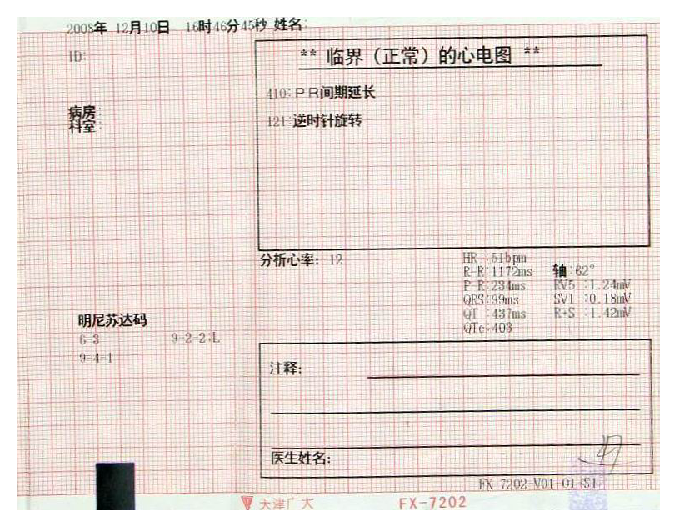
\epsfig{file=figure/f2.eps, width=0.24\columnwidth}
}
%\hfill
\subfloat[Format 3]{
\label{fig:dataset:3}
\epsfig{file=figure/f3.eps, width=0.24\columnwidth}
}
\subfloat[Format 4]{
\label{fig:dataset:4}
\epsfig{file=figure/f4.eps, width=0.24\columnwidth}
}
\caption{Examples of Four Kinds of ECGs}
\label{fig:dataset}
\end{figure}

\begin{table}[th]
\centering
\caption{Statistics for The Dataset}
\label{tab:statis}
\begin{tabular}{|c|c|c|c|c|}
\hline
Format & 1 & 2 & 3 & 4\\
\hline \hline
Number of Images & 124 & 113 & 102 & 97\\ 
\hline
Number of Attributes per Image & 17 & 16 & 18 & 15 \\
\hline
\end{tabular}
\end{table}

As the examples shown, these ECG images are in different colors 
and have many noises like grid lines. 
Because these variations and noises affect the performance of the OCR engine, 
we preprocess the images into a clean version. 
The detailed techniques are discussed in \secref{sec:discuss}. 

% we use auto thresholding to 
% preprocess the images to remove the noisy lines and 
% turn the color images into black and white. 
% An example of the preprocessing result is shown in \figref{fig:preprocess}. 
% Auto thresholding is to segment the images based on the colour 
% features automatically. In our system we make use of the tool 
% ImageJ\cite{schneider2012671} to do the preprocessing.  
% \begin{figure}[ht]
% \centering
% \subfloat[Before Preprocessing]{
% \label{fig:preprocess:1}
% \epsfig{file=figure/f1.eps, width=0.48\columnwidth}
% }
% % \hfill
% \subfloat[After Preprocessing]{
% \label{fig:preprocess:2}
% \epsfig{file=figure/pref1.eps, width=0.48\columnwidth}
% }
% \caption{Results of Preprocessing}
% \label{fig:preprocess}
% \end{figure}

\subsection{Extraction Accuracy}
Next, we compare our method with three competing methods.
The first and most naive method for information extraction from medical images 
is to write a simple parser for the XML results of the OCR engine. 
We consider this approach to be the baseline for 
evaluation. In this parser, we didn't include any fuzzy matching 
strategies, but instead extracted all results using exact matches. 

The second competing method involves marking all zones of interest 
on images and getting all the OCR results in them. 
To adjust the small changes of 
zone areas between images, a marker zone is set so that 
all other zones of interest can be adjusted against it as
a reference point. 
An example image after being marked with the zones of interest 
and the marker zone is shown in \figref{fig:zOCR} (Zones of interest 
are in blue and the marker zone is in red).

\begin{figure}[th]
\begin{minipage}{0.5\columnwidth}
\centering
\epsfig{file=figure/17_zOCR.eps, width=0.7\columnwidth}
\caption{Image Marked With Zones}
\label{fig:zOCR}
\end{minipage}
\begin{minipage}{0.5\columnwidth}
\centering
\epsfig{file=figure/17_pl.eps, width=0.7\columnwidth}
\caption{Page Layout Analysis Result}
\label{fig:pl}
\end{minipage}
\end{figure}

The third approach is to use the page layout analysis 
technique \cite{o1993document}. 
This method is used to determine where the text 
resides on a page. 
By this method, the hierarchy of physical components 
can be generated against which we can match the predefined 
hierarchy of logical components. An example result of our page layout 
analysis is shown in \figref{fig:pl}.

\begin{figure}[th]
\centering
\epsfig{file=figure/2_pl.eps, width=0.5\columnwidth}
\caption{An Error Page Layout Analysis Result}
\label{fig:errorpl}
\end{figure}


The results of comparison are shown in \tabref{tab:compare}. 
We only calculated the accuracies for extracting the results of 
variables since we already know the exact values of constant 
expressions. Based on our experiment, our method of fuzzy matching 
outperforms all other methods on all 4 types of ECGs. 
The reason is that zonal OCR and page layout analysis are highly 
related to image processing in order to extract data. The accuracy of 
zonal OCR is greatly affected by the setting of zones of interest. 
If the zones of interest are too large, it's possible that noises are
also extracted; while if the zones of interest are too small, results 
can be incomplete. For page layout analysis, the accuracy is 
affected by the granularity of the page layout unit and the 
misrecognition affects the matching with the predefined 
hierarchy of logical components. For our method, the smallest 
unit is word in text so our description can be very accurate. 
At the same time, the fuzzy matching strategies also enable 
the description to omit some unnecessary details.
% \KZ{Need focus on explaining why we are only slightly better, and what are
% the problems of the other three methods, despite that their accuracies are
% not that bad! e.g., efforts to mark the zones, I'm still not convinced
% how come without fuzzy match, zonal methods can be so good since the dist
% between the marker zone and the interesting zones can be slightly off in each
% image.}   

Even though the two competing approaches seem just marginally outperformed
by our fuzzy matching approach, these two approaches have their own 
important limitations. 
In a zonal OCR, it's important to adjust the zones of interest 
based on the marker zone. Misrecognition of the marker 
is disasterous, as all the extracted information will be incorrect. 
The other approach, page layout analysis, requires analyzing 
the text boxes in images before conducting logical labeling. 
If the text boxes are recognized incorrectly, some of the
important information may be omitted from output. 
As shown in \figref{fig:errorpl}, 
text box recognition errors cause the OCR to overlook the unit and 
other valuable information. 
However, the fuzzy match design of our system can 
tolerate these types of errors that the OCR engine often makes. 
We seek to find an optimized solution which can extract 
correct information as much as possible. 


\begin{table}[th]
\centering
\caption{Accuracy For Different Methods}
\label{tab:compare}
\begin{tabular}{|c|c|c|c|c|}
\hline
Format & 1 & 2 & 3 & 4\\
\hline \hline
Exact Match & 58.8\% & 56.3\% & 61.1\% & 53.4\% \\
\hline
Zonal OCR & 81.2\% & 79.8\% & 81.7\% & 80.6\% \\
\hline
Page Layout & 79.7\% & 80.2\% & 81.2\% & 81.1\% \\
\hline
Our Fuzzy Match & {\bf 85.5\%} & {\bf 83.8\%} & {\bf 84.9\%} & {\bf 84.0\%}\\ 
\hline
\end{tabular}
\end{table}

\subsection{Incremental Manual Correction}
%In this section, we compare the performance of 
%the human correction part in our system. 
%Another important part of our system is the human correction 
%process. By making use of the human power, we can correct 
%the errors that occur due to the OCR engine. 
We compare the two policies for recommending errors for manual correction, 
namely, random recommendation and most frequent error 
description element recommendation. The relationship between the 
amount of corrections and the accuracy of different types of 
ECGs are shown in \figref{fig:humancorr}. 
%For random correction, we randomly suggest that some errors be 
%corrected each time. 
%The accuracy of random correction is calculated by averaging 
%the results 100 times. For the most frequent error 
%description element recommendation, 
%corrections for most frequently made errors will be suggested first. 

%\KZ{Some of the words are incorrectly displayed in the following figures.}

\begin{figure}[!ht]
\centering
\subfloat{
%% \label{fig:hc:1}
\epsfig{file=figure/hcf1.eps, width=0.48\columnwidth}
}
% \hfill
% \centering
\subfloat{
% \label{fig:hc:2}
\epsfig{file=figure/hcf2.eps, width=0.48\columnwidth}
}
\hfill
% % \centering
\subfloat{
% \label{fig:hc:3}
\epsfig{file=figure/hcf3.eps, width=0.48\columnwidth}
}
% % \centering
\subfloat{
% \label{fig:hc:4}
\epsfig{file=figure/hcf4.eps, width=0.48\columnwidth}
}
\caption{Comparison of Two Correction Strategies in 4 Types of Images}
\label{fig:humancorr}
\end{figure}

% \KZ{Need to modify the figs so that lines don't touch into
% the legends, ad the caption don't overlap with the figs.}

As shown in \figref{fig:humancorr}, the more corrections we make, 
the better accuracy we get. 
The improvement to the accuracy rate is better 
when using the most frequent recommendation, compared with random 
recommendation. Using the most 
frequent recommendation is more effective, 
since we can correct more errors than random recommendation. 
With more corrections made, the improvement of 
accuracy tends to saturate, especially with regard to the 
most frequent error strategy. This is the effect of diminishing
returns, as corrections learned later tend to be minor ones and make
less impact to the overall performance.
% \KZ{Need to explain why there's only limited improvement after 15 corrections.
% Maybe because the data size is not big enough, so there's not many repeated
% errors?}
The improvement of accuracy is limited after 15 corrections. 
The main reason is that there are not many repeated errors due to 
the small size of the data set and furthermore, our system 
can only make corrections according to the correction model, 
which is sensitive to repeated errors.

% \begin{enumerate}
% \item Compare the description code with generated code to show our language is a simple one;
% \item Compare the accuracy with baseline, exact match on the OCR results, to show our language can tolerate the noises and errors;
% \item Compare the performance on different image formats;

% \item Compare the accuracy between our approach and others, including using related image position;


% \item Experiments about the relationship of the accuracy rate 
% and the number of errors corrected;

% \begin{table}[!hbp]
% \centering
% \caption{Most Frequent}
% \begin{tabular}{|c|c|c|c|c|}
% \hline
% Type & 1 & 2 & 3 & 4\\
% \hline
% Accuracy(0 errors) & 85.5\% & 83.8\% & 84.9\% & 84.0\%\\ 
% \hline
% Accuracy(1 errors) & 85.7\% & 84.0\% & 85.0\% & 84.2\%\\ 
% \hline
% Accuracy(5 errors) & 86.2\% & 84.6\% & 85.6\% & 84.8\% \\
% \hline
% Accuracy(10 errors) & 86.6\% & 85.2\% & 86.2\% & 85.5\% \\
% \hline
% Accuracy(15 errors) & 86.8\% & 85.7\% & 86.6\% & 85.9\% \\
% \hline
% % \caption{Most Frequent}
% \end{tabular}
% \end{table}

% 0 85.5 85.5
% 1 85.7 85.5
% 5 86.2 85.7
% 10 86.6 86.0
% 15 86.8 86.2

% 0 83.8 83.8
% 1 84.0 83.9
% 5 84.6 84.1
% 10 85.2 84.4
% 15 85.7 84.7

% 0 84.9 84.9
% 1 85.0 84.9
% 5 85.6 85.1
% 10 86.2 85.4
% 15 86.6 85.7

% 0 84.0 84.0
% 1 84.2 84.1
% 5 84.8 84.4
% 10 85.5 84.7
% 15 85.9 85.1

% \begin{table}[!hbp]
% \centering
% \caption{Random}
% \begin{tabular}{|c|c|c|c|c|}
% \hline
% Type & 1 & 2 & 3 & 4\\
% \hline
% Accuracy(0 errors) & 85.5\% & 83.8\% & 84.9\% & 84.0\%\\ 
% \hline
% Accuracy(1 errors) & 85.5\% & 83.9\% & 84.9\% & 84.1\%\\ 
% \hline
% Accuracy(5 errors) & 85.7\% & 84.1\% & 85.1\% & 84.4\% \\
% \hline
% Accuracy(10 errors) & 86.0\% & 84.4\% & 85.4\% & 84.7\% \\
% \hline
% Accuracy(15 errors) & 86.2\% & 84.7\% & 85.7\% & 85.1\% \\
% \hline
% % \caption{Random}
% \end{tabular}
% \end{table}


% \begin{figure}
% \centering
% \subfloat[ECG1]{
% \label{fig:hcre:a}
% \epsfig{file=figure/f1.eps, width=0.48\columnwidth}
% }
% \hfill
% \subfloat[ECG2]{
% \label{fig:hcre:b}
% 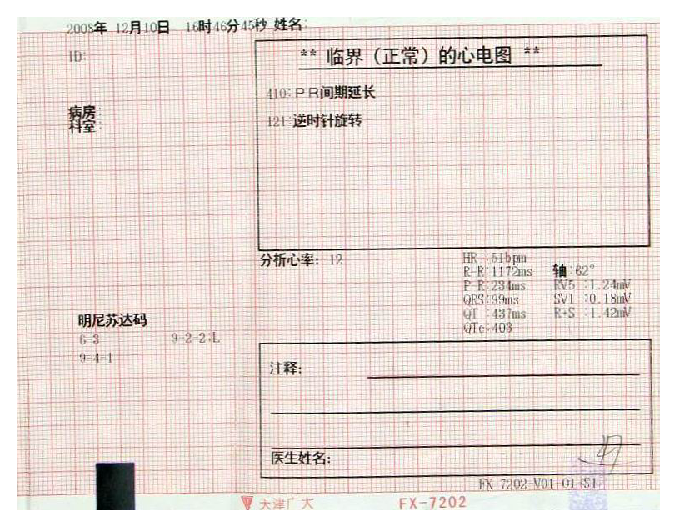
\epsfig{file=figure/f2.eps, width=0.48\columnwidth}
% }
% \hfill
% \subfloat[ECG3]{
% \label{fig:hcre:c}
% \epsfig{file=figure/f3.eps, width=0.48\columnwidth}
% }
% \hfill
% \subfloat[ECG4]{
% \label{fig:hcre:d}
% \epsfig{file=figure/f4.eps, width=0.48\columnwidth}
% }
% % \caption{E}
% \label{fig:hcre}
% \end{figure}

% \item Compare different strategies for correcting errors, including most frequent error elements, most frequent error types.
% \end{enumerate}

\section{Discussion}
\label{Discussion}


\section{Related Work}
\paragraph{Clarification Question Generation} The concept of CQ can be naturally raised in a dialogue system where the speech recognition results tend to be erroneous so that we raise CQs for sanity check \citep{stoyanchev2014towards}, or the intents for a task is incomplete or ambiguous in a first short utterance and further CQs are needed to fill in the slots \citep{dhole2020resolving}. The concept is then extended to IR to clarify ambiguous queries \citep{aliannejadi2019asking}, and has been successfully put into practice \citep{zamani2020generating}. Other application areas including KBQA \citep{xu2019asking} and open-domain dialogue systems \citep{aliannejadi2020convai3}. CQGen can also be applied to help refine posts on websites like StackExchange \citep{Kumar_2020} and Amazon \citep{rao2019answer}. In this context, our work closely follows the research line of \citep{rao2018learning, rao2019answer, cao2019controlling}. \citet{rao2018learning} first adopted a retrieval-then-rank approach. They \citep{rao2019answer} then proposed a generation approach to train the model to maximize the utility of the hypothetical answer for the questions with GAN, to better promote specificity. \citet{cao2019controlling} propose to control the specificity by training on data with explicit indicator of specificity, but it requires additional specificity annotation. Towards the similar specificity goal, we adopted a different keyword-based approach. They also assume generating one question per context, which we claim is not sufficient to cover various possible information needs, and thus propose the task of the diverse CQGen.

\paragraph{Diverse Generation} The demand for diverse generation exists in many other fields~\cite{vijayakumar2018diverse, LiangZ18code, shen2019mixture}, and we've drawn inspirations from these literatures. For image captioning, we may use multiple descriptions for different focusing points of a scene. \textit{Diverse Beam Search} \citep{vijayakumar2018diverse} was proposed to broaden the searching space to catch such diversity by dividing groups in decoding and imposing repetition penalty between them. For machine translation, a context can be translated with different styles. \citet{shen2019mixture} thus proposed \textit{Mixture of Expert} models including hMup to reflect various styles with a discrete latent variable (\textit{expert}). And here for CQGen, diversity is required to cover various potentially missing aspects, so we come up with the idea to use keywords as a controlling variable like \textit{expert} to promote diversity.


\section{Conclusion}

In this paper, we incorporated the idea of Cookie Theft picture description task into the evaluation of the high-level cognitive abilities of LVLMs and designed a novel evaluation benchmark called CogBench.
% Images in CogBench are of high quality and require more cognitive reasonings to understand, which makes it different from existing image datasets.
The images in CogBench are of high quality and demand more complex cognitive reasoning for interpretation, setting it apart from existing image datasets.
% It consists of a image description task and a VQA task.
Experiments show that there is still a large gap between the cognitive abilities of LVLMs and human beings, indicating CogBench is a challenging benchmark.

% In the future


% \IEEEraisesectionheading{
% % %\IEEEraisesectionheading{
% %\IEEEraisesectionheading{
% %\IEEEraisesectionheading{
% \input{intro}
\section{Introduction}\label{sec:intro}
 %}
% \section{Introduction}\label{sec:intro}

% \begin{enumerate}
% \item Motivation: application scenarios (with 1-2 running examples);
% \item Characteristics of the data sources and their challenges;
% \item Briefly introduce previous approaches to extract information 
% from images including setting the document zone, and their limitations.
% \item General flow of our approach (may give a diagram here)
% \end{enumerate}
% scenary

Due to ever evolving hardware and software, many medical images
such as electro-cardio graphs (ECGs), X-ray or ultrasound images  
are directly printed and stored in hard copy formats. 
% \KZ{Insert 4 example images here.}
%Examples are shown in \figref{fig:medicalImages}. 
% These images often contain a mix of graphics and text, which
% include parameter settings of the hardware, test measurements or simple
% diagnosis. 
These images often contain a mix of graphics and text, which 
include technical settings of the hardware used, test measurements or simple diagnoses.
Recently, there has been a growing demand for digitizing such 
medical information from paper media sources, especially legacy ones, or patients who want to keep track of these documents by themselves digitally. 
Apart from scanning the graphics into a digital format, extracting 
the semi-structured textual information is also an important part of
building electronic medical records for patients. 

%\begin{figure}[!htb]
%\centering
%\subfloat[ECG]{
%\label{fig:medicalimage:ecg}
%\epsfig{file=figure/17_ori.eps, width=0.4\columnwidth}
%}
%% \hfill
%\subfloat[MRI]{
%	\label{fig:medicalimage:mrt}
%	\epsfig{file=figure/MRI.eps, width=0.4\columnwidth}
%}
%\\
%\subfloat[X-RAY]{
%\label{fig:medicalimage:xray}
%\epsfig{file=figure/X-RAY.eps, width=0.4\columnwidth}
%}
%%\hfill
%\subfloat[EEG]{
%\label{fig:medicalimage:eeg}
%\epsfig{file=figure/EEG.eps, width=0.4\columnwidth}
%}
%\caption{Examples of Medical Images}
%\label{fig:medicalImages}
%\end{figure}

Optical character recognition (OCR)  \cite{mori1992historical,smith2007overview} is 
a traditional technique used to turn images of printed text into machine encoded
text. It is well researched and performs well on plain text 
documents such as novels and reports, for a variety of languages. 
%For example, Tesseract, which is one of 
%the most popular open source multilingual recognizers, logs an error 
%rate of 3.72\% for English words and 3.77\% for simplified 
%Chinese characters\cite{smith2009adapting}. 
%Google Books \cite{googlebooks} and Gutenberg \cite{gutenberg} are
%projects which have scanned a large number of paper books into text for free and open
%access. These projects made exclusive use of OCR for this conversion and 
%achieved high accuracy \cite{vincent2007google} \cite{lebert2008project}. 
% 99\% for Gutenberg project \cite{lebert2008project}. 
% \KZ{Give the accuracy of google and gutenberg if available.}


\begin{figure}[th]
\centering
\epsfig{file=figure/17_b.eps, width=0.8\columnwidth}
\caption{An ECG image with text area (red circle) of interest.}
\label{fig:ecgexample2}
\end{figure}

For a semi-structured medical image, such as 
\figref{fig:ecgexample2}, we would like to extract the attribute-value 
pairs (e.g., {\em Vent. rate = 63 bpm}) and possibly other values such as
date ({\em 18-Nov-2010}) and time ({\em 9:13:02}) since those values endow us with lots of information about the patient. 
Existing OCR software cannot extract such structured information in a straightforward 
fashion, 
but instead it produces rather convoluted results from the whole image, 
similar to those in \figref{fig:ocrre}, which was produced by Tesseract, 
a popular multi-lingual recognizers. 
% \KZ{Maybe include the x-y coordinate info in the output as well?}  

\begin{figure}[th]
\centering
\scriptsize
\begin{verbatim}
<p class="ocr_par" title="box 263 33 444 119">
   <span class="ocr_l" title="box 264 33 336 45">
       <span class="ocrx_w" title="box 264 33 299 45">Vcnt.</span> 
       <span class="ocrx_w" title="box 308 34 336 45">rule</span> 
   </span>
   <span class='ocr_l'>
       <span class="ocrx_w" title="box 264 51 283 64">PR</span> 
       <span class="ocrx_w" title="box 291 51 346 64">Interval</span> 
       <span class="ocrx_w" title="box 389 52 411 64">140</span> 
       <span class="ocrx_w" title="box 420 55 439 64">ms</span> 
   </span>
   ...
   </span>
</p>
<p class="ocr_p" dir="ltr">
   <span class="ocr_l">
       <span class="ocrx_w" title="box 396 33 411 45">53</span> 
       <span class="ocrx_w" title="box 420 33 449 48">bpm</span> 
   </span>
</p>
\end{verbatim}
\caption{Snippet OCR results in XML, input to our framework.}
\label{fig:ocrre}
\end{figure}


%\input{xmlre1}

%However, OCR alone does not work well on semi-structured text and hence
%can't be directly used for information extraction from the aforementioned
%medical images. \KZ{Give the reason here, perhaps because OCR models are
%largely Markov based? So semi-structured data breaks the flow of text.}
%When a medical image is input to an ordinary OCR software, the spatial 
%information of the text components is often lost or mixed with noises
%and errors.
%%The reason is OCR converts the whole images into text data, in which 
%%useful information often mix with noises and errors. 
%In this paper, we would like to extract the attribute-value pairs
%and possibly other values from \figref{fig:ecgexample1} 
%and \figref{fig:ecgexample2}. 
%% or medical ultrasonography report. 
%Such images contain lots of non-textual information or noises.

% example & ref
%\begin{figure}[ht]
%\centering
%\epsfig{file=figure/46.eps, width=0.8\columnwidth}
%\caption{ECG Images From Printer1}
%\label{fig:ecgexample1}
%\end{figure}

% \begin{figure}[ht]
% \centering
% \subfloat[Printer1]{
% \label{fig:ecgexample:a}
% \epsfig{file=figure/46.eps, width=0.48\columnwidth}
% }
% \hfill
% \subfloat[Printer2]{
% \label{fig:ecgexample:b}
% \epsfig{file=figure/17.eps, width=0.48\columnwidth}
% }
% \caption{ECG images from two different printers}
% \label{fig:ecgexample}
% \end{figure}

Also, errors in the OCR text \cite{darwish2007error,taghva1996evaluation} will greatly affect the effectiveness 
of other related tasks. Much work has been done to improve the performance of the OCR\cite{kolak2003generative,cesarini1998informys}. However, there are still a number of significant challenges involved in extracting the information from medical images or OCR results in XML form. 

% First, medical images differ from pure text document in that them have 
% layout information. 
First, medical images differ from pure text documents in that 
they contain layout information.
Although most current OCR engines attempt to reproduce the physical 
layout of the text units, 
%(along with X-Y coordinates) and store them 
%in a special format such as XML 
% (\KZ{Better in the previous example})
such spatial
information is approximate and sometimes inaccurate, which is why neighboring
text blocks in \figref{fig:ecgexample2}, such as ``Vent. Rate'' and
``63 bpm'' were not automatically combined into the same XML block, but were 
rather far apart (shown in two different ``classes'') in \figref{fig:ocrre} made by OCR softwares. 
%Even for images produced by the same ECG printer, 
%the XML results can still be very different as 
The spatial layout is sensitive to many factors, such as accidental spots 
on the prints, color and contrast, or the angle of the camera. 
%In this case, solutions for other application domains, for example, the web, 
%are not well suited for information extraction from printed documents \cite{bartoli2014semisupervised}. With such inaccurate
%layout information produced by OCR,
%it is not easy to write a simple wrapper program to extract useful
%data from images, even if the images come from the same printer. 

%Writing a wrapper for each
%individual image would be tedious and counter-productive. Therefore,
%a mechanism that makes use of the spatial locality of the 
%text units in the image and 
%accommodates slight variations in the spatial layout would make the extraction
%more accurate and fault-tolerant.

%For example, \figref{fig:ocrre} is the simplified OCR results for the ECGs in 
%\figref{fig:ecgexample1} and \figref{fig:ecgexample2}. The results are in the XML format and have attritube named {\em class} 
%for layout information. Although these two images share similar format. 
%OCR engine generates different results in that it splits elements that 
%should be in the same line into two lines in the second example. 
%XML is sensitive to the layout results so it's hard to tolerate 
%all the layout results. 
%
% example check the term
% layout of ocr results can be restore, so why OCR engine don't restore the results 
% using the similar methods as we do?
% or the way we handle the layout problem is quite simple

% Delete for TIP
% Second, exiting OCR engines make heavy use of Markov properties such as n-grams
% since they primarily target the transformation of large body of text 
% \cite{kolak2003generative}. 
% % \KZ{Needs some refs here.}
% Unfortunately, the semi-structured texts in medical images are often 
% short and not even written in complete sentences, thus breaking Markov assumption. To make
% matters worse, medical images contain scientific language, which may be
% very different from the training corpora of these OCR engines.
% This explains why we see errors like ``Vcnt'' and ``rule'' 
% in \figref{fig:ocrre}. 
% %can't guarantee a perfect performance, which means 
% %there are errors and noises in the OCR results.
% %Many of them due to the fact that the data are no longer long, continous
% %sentences, thus breaking the Markov assumption made by many OCR algorithms. 
% %In \figref{fig:ocrresub:b}, ``Vent." is misrecognized as ``Vcnt.". 
% Without sufficient contextual information, OCR may also misrecognize a 
% digit as an alphabetic character, or as another similar digit. 
% Furthermore, the mix of text with images and formatting
% lines often confuses the OCR engine, which is more biased toward full
% text images.
% Exact pattern matching, as used in
% traditional information extraction, doesn't work with such noisy OCR output
% as it doesn't tolerate noises or errors in text. 
% %It's hard to autocorrect these errors 
% %because image quality is the most important affecting factor. 
% %The text we are processing can be full of no meaning words or 
% %strange numbers. 
% A fuzzy matching strategy is more desirable in this case. 
% % example, what are the traditional IEs

Second, there are many types of medical images, resulting from a variety of
medical tests. Different equipments for the same test can produce vastly 
different images. Writing individual extraction wrappers 
for the OCR outputs of all these formats is tedious and inefficient, 
and difficult for non-programmers.
%not to mention that there are significant programming barriers for 
%writing these wrappers, especially for the medical professionals who are the
%end users of these extraction results. 
%A more user-friendly approach enabling users to specify such extraction requirements would be preferred. 
%There are various kinds of medical images, such as electrocardiograph report, 
%medical ultrasonography report, etc. 
%However the basic measures for each type of medical test (e.g., ECG), 
%are very similar from machine to machine. Only the layouts are 
%different. 
% example medical images

Finally, most off-the-shelf OCR programs are pre-trained with specific 
recognition models, which may not be suitable for the extraction of 
%medical images.
%Furthermore, changes in imaging equipment technology over time may produce 
%different formats, layout, or terminology, rendering existing OCR models 
%obsolete. 
Re-training the models requires a large amount of labeled data, which may
not be available. 
%Incremental training as more labeled data arrives
%is currently not supported by any OCR product.    

%There have been some limited attempts to address some of the above challenges. 
%One solution is a plugin of an OCR program that allows the user to specify 
%target zones of interest in the image to be extracted. The zones specified for
%one image can be applied to images with slight variations by adjusting against
%a fixed reference point that is supposed to exist in all these images.
%% \KZ{I think the problem is not so much with the zones, because we also
%% have zones, but rather with the reference point.}
%% \JY{}
%% example products
%% http://www.square-9.com/automated-data-extraction-optical-character-recognition
%The problem with this solution is its high reliance on the OCR zones  
%established by the user. The performance of the results is affected by the 
%accuracy of the zones. If the zones are too big, the results will be full of 
%noise. If the zones are too small, results will miss something. 
%
%Another solution involves using the page layout analysis technique. The page layout 
%analysis technique is used to determine where the text 
%resides on a page \cite{o1993document}, 
%% \KZ{This page layout analysis approach is not clearly described. I don't understand after reading this paragraph.}
%% By using page layout analysis technique, the hierarchy of physical components 
%% can be generated and to match with the hierarchy of logical components, which 
%% is predefined. 
%this includes identifying and categorizing the 
%regions of interest in the scanned image of a text document. 
%Typically, the first step is to segment text zones from 
%non-textual zones and arrange them in their original order. 
%Then in order to analyze the logical roles of the text zones 
%(titles, captions, footnotes, etc.), logical layout analysis 
%is used for labeling the semantics of the text zones.
%Generally, page layout analysis is used for documents. The problem with applying 
%such a technique on medical images is that it creates so much noises 
%that performance is ultimately affected. 
%For medical imaging reports like ECG, useful information is often 
%found in the small components of the image, while most of the images are 
%read as noises. 
% check paper and more description, weakness, ref

%In this paper, 
%we propose a spatial data description language, which borrows its syntax from
%PADS \cite{fisher+:pads}, an ad hoc data processing language, 
%for describing semi-structured data in medical images. 
%% ref
%We call this language OCR description language, or ODL. 
%ODL is designed for extracting and parsing semi-structured text data 
%from images. We believe that  information extraction from those data in ODL form may be much easier than extracting information from rough data or data in XML form, which means that our preprocessing part proves to be necessary.
%%An example ODL description for the image in 
%%\figref{fig:ecgexample2} is shown in 
%%\figref{fig:description}. \KZ{Make this description two column, and give
%%some brief explanation of this description here.} 
%%The parsing result of this description is shown
%%in \figref{fig:parsing result}. \KZ{Give some explanation of the results,
%%otherwise don't show the result here. E.g., you need to explain what F, E, etc.
%%mean. You want to say that even though rate has been recognized as rule,
%%the bpm value was still extracted (but still wrong!).}
%% \KZ{I removed the preprocessing part, cos it's not important. Talk about it in
%% discussion sec.}
%%The our approach starts by preprocessing the images for text results.
%To use this framework, the user first describes the components in the image
%that he or she is interested in extracting. This includes constant strings
%and variables of different data types.   
%ODL allows the user to specify the approximate spatial layout and constraints on
%the data, e.g., integers within 
%a certain range, real numbers with certain decimal points, etc. 
%%This information is then as the key component in our fuzzy matching strategy. 
%The system then automatically generates a parser for these medical images.
%This parser uses the output XML from OCR with spatial information as an input, 
%and outputs a data structure with values extracted for each variables
%in the description, unless there is an unrecoverable error during the parsing process.
%In addition, approximate layout information and constraints are used in parsing process 
%to tolerate noises and small format variations in the input images. 
%%Specifically, this method could be called fuzzy matching, meaning that more candidates could be saved after the parsing process.  It's obvious that we may have a higher probability to obtain the accurate result if more candidates are kept so that fuzzy match should be used properly in our system.
%%An autogenerated parser based on the ODL description can release us from 
%%repetitive work. In this way, we turn the task of writing complex parsers 
%%into describing information on images.
%
%
%When users process many images of the same format, the system 
%automatically discovers parsing errors given the current model and 
%prompts the user to manually correct some of the frequent and prominent
%errors, which effectively serves as an online labeling function. 
%These incrementally labeled data are then used to update the parsing model. 


%It should be emphasized that the incremental learning model is very important in our whole system. Incremental learning is a machine learning paradigm where the learning process takes place whenever we have new examples or data added to our baisc data set, leading to a most striking difference between incremental learning and traditional machine learning: it does not assume the availability of a sufficient training set before the learning process. What incremental learning in our system is really impressive: it does not require a relatively good and stable training set at first time. In fact, it could improve the parsing result with even relatively rough training sets at first by absorbing new data or corrective information as time passes in dynamic systems. Besides, the process would be very effective when there are some new images coming in since training process would not learn from scratch, which might waste time and computation resource.

%At last, we propose an incrementally human correction framwork which can 
%make the best use of human correction to handle the misrecognition problem. 
% Base on our experiments on about 500 real life ECG images, 
% our approach achieves p1 and p2 after p3 times human correction. 
% experimental results

% \begin{figure}[h]
% \begin{lstlisting}
% Oenum str_month_t{
% 	"Jan", "Feb", "Mar", "Apr",
% 	"May", "Jun", "Jul", "Aug",
% 	"Sept", "Oct", "Nov", "Dec"
% };

% Ounion month_t{
% 	Oint(1,12)	num;
% 	str_month_t	str;
% };

% Ostruct time_t{
% 	Oint(1,31)	day;
% 	"-";
% 	month_t	month;
% 	"-";
% 	Oint	year;
% };

% Ostruct triple_t{
% 	"Vent.";
% 	hskip(\s)	skip1;
% 	"rate";
% 	Oint x;
% 	"bpm";
% 	vskip(\n)	skip2;
% };

% Oscource Ostruct entry_t{
% 	time_t(<-,-,-,0.3l>) t;
% 	triple_t(<0.1w,-,0.5w,->) d;
% };
% \end{lstlisting}
% \caption{Description}\label{fig:description}
% \end{figure}


In order to solve above problems, We design a system which makes three main contributions:
\begin{enumerate}
\item Based on some previous work on data description language \cite{lamport1986document,taft1999post,fisher+:pads},we design a new declarative spatial data description language called \textit{OCR description language}, or ODL,
which allows users to specify spatial and data constraints in medical 
images(\secref{sec:syntax});
\item We propose a noise-tolerant parser which takes OCR results
the ODL description as input and outputs a data structure with values 
extracted for each variables in the description (\secref{sec:semantics});
\item We propose an incremental manual correction 
framework\cite{von2008recaptcha,zhu2012learnpads++}, which 
takes advantage of user corrections  and improves the productivity
significantly (\secref{sec:correction}).
%To be more specific, the framework improves the traditional machine learning methods by using a incremental learning process to avoid starting from scratch when we are trying to apply human corrections in the system. That means the framework would be more effective than most corrective systems.
\end{enumerate}


\section{Introduction}\label{sec:intro}
 %}
% \section{Introduction}\label{sec:intro}

% \begin{enumerate}
% \item Motivation: application scenarios (with 1-2 running examples);
% \item Characteristics of the data sources and their challenges;
% \item Briefly introduce previous approaches to extract information 
% from images including setting the document zone, and their limitations.
% \item General flow of our approach (may give a diagram here)
% \end{enumerate}
% scenary

Due to ever evolving hardware and software, many medical images
such as electro-cardio graphs (ECGs), X-ray or ultrasound images  
are directly printed and stored in hard copy formats. 
% \KZ{Insert 4 example images here.}
%Examples are shown in \figref{fig:medicalImages}. 
% These images often contain a mix of graphics and text, which
% include parameter settings of the hardware, test measurements or simple
% diagnosis. 
These images often contain a mix of graphics and text, which 
include technical settings of the hardware used, test measurements or simple diagnoses.
Recently, there has been a growing demand for digitizing such 
medical information from paper media sources, especially legacy ones, or patients who want to keep track of these documents by themselves digitally. 
Apart from scanning the graphics into a digital format, extracting 
the semi-structured textual information is also an important part of
building electronic medical records for patients. 

%\begin{figure}[!htb]
%\centering
%\subfloat[ECG]{
%\label{fig:medicalimage:ecg}
%\epsfig{file=figure/17_ori.eps, width=0.4\columnwidth}
%}
%% \hfill
%\subfloat[MRI]{
%	\label{fig:medicalimage:mrt}
%	\epsfig{file=figure/MRI.eps, width=0.4\columnwidth}
%}
%\\
%\subfloat[X-RAY]{
%\label{fig:medicalimage:xray}
%\epsfig{file=figure/X-RAY.eps, width=0.4\columnwidth}
%}
%%\hfill
%\subfloat[EEG]{
%\label{fig:medicalimage:eeg}
%\epsfig{file=figure/EEG.eps, width=0.4\columnwidth}
%}
%\caption{Examples of Medical Images}
%\label{fig:medicalImages}
%\end{figure}

Optical character recognition (OCR)  \cite{mori1992historical,smith2007overview} is 
a traditional technique used to turn images of printed text into machine encoded
text. It is well researched and performs well on plain text 
documents such as novels and reports, for a variety of languages. 
%For example, Tesseract, which is one of 
%the most popular open source multilingual recognizers, logs an error 
%rate of 3.72\% for English words and 3.77\% for simplified 
%Chinese characters\cite{smith2009adapting}. 
%Google Books \cite{googlebooks} and Gutenberg \cite{gutenberg} are
%projects which have scanned a large number of paper books into text for free and open
%access. These projects made exclusive use of OCR for this conversion and 
%achieved high accuracy \cite{vincent2007google} \cite{lebert2008project}. 
% 99\% for Gutenberg project \cite{lebert2008project}. 
% \KZ{Give the accuracy of google and gutenberg if available.}


\begin{figure}[th]
\centering
\epsfig{file=figure/17_b.eps, width=0.8\columnwidth}
\caption{An ECG image with text area (red circle) of interest.}
\label{fig:ecgexample2}
\end{figure}

For a semi-structured medical image, such as 
\figref{fig:ecgexample2}, we would like to extract the attribute-value 
pairs (e.g., {\em Vent. rate = 63 bpm}) and possibly other values such as
date ({\em 18-Nov-2010}) and time ({\em 9:13:02}) since those values endow us with lots of information about the patient. 
Existing OCR software cannot extract such structured information in a straightforward 
fashion, 
but instead it produces rather convoluted results from the whole image, 
similar to those in \figref{fig:ocrre}, which was produced by Tesseract, 
a popular multi-lingual recognizers. 
% \KZ{Maybe include the x-y coordinate info in the output as well?}  

\begin{figure}[th]
\centering
\scriptsize
\begin{verbatim}
<p class="ocr_par" title="box 263 33 444 119">
   <span class="ocr_l" title="box 264 33 336 45">
       <span class="ocrx_w" title="box 264 33 299 45">Vcnt.</span> 
       <span class="ocrx_w" title="box 308 34 336 45">rule</span> 
   </span>
   <span class='ocr_l'>
       <span class="ocrx_w" title="box 264 51 283 64">PR</span> 
       <span class="ocrx_w" title="box 291 51 346 64">Interval</span> 
       <span class="ocrx_w" title="box 389 52 411 64">140</span> 
       <span class="ocrx_w" title="box 420 55 439 64">ms</span> 
   </span>
   ...
   </span>
</p>
<p class="ocr_p" dir="ltr">
   <span class="ocr_l">
       <span class="ocrx_w" title="box 396 33 411 45">53</span> 
       <span class="ocrx_w" title="box 420 33 449 48">bpm</span> 
   </span>
</p>
\end{verbatim}
\caption{Snippet OCR results in XML, input to our framework.}
\label{fig:ocrre}
\end{figure}


%% \begin{figure}[ht]
% \centering
% \subfigure[]{
% \label{fig:subfig:a}
% \begin{minipage}[b]{0.2\textwidth}
%\newsavebox{\firstlisting}
%\begin{lrbox}{\firstlisting}% Store first listing
%\begin{lstlisting}
%<p class='ocr_par' dir='ltr'>
%   <span class='ocr_line' id='line_2'>
%       <span class='ocrx_word' id='word_6'>Vent.</span>
%       <span class='ocrx_word' id='word_7'>rate</span>
%       <span class='ocrx_word' id='word_8'>65</span>
%       <span class='ocrx_word' id='word_9'>bpm</span>
%   </span>
%   <span class='ocr_line' id='line_3'>
%       <span class='ocrx_word' id='word_14'>PR</span>
%       <span class='ocrx_word' id='word_15'>interval</span>
%       <span class='ocrx_word' id='word_16'>162</span>
%       <span class='ocrx_word' id='word_17'>ms</span>
%   </span>
%    ...
%</p>
%\end{lstlisting}
%\end{lrbox}
% \end{minipage}
% }
% \hspace[1in]
% \subfigure[]{
% % \label{fig:subfig:b}
% % \begin{minipage}[b]{0.2\textwidth}
\newsavebox{\secondlisting}
\begin{lrbox}{\secondlisting}
% \tiny
\begin{lstlisting}[basicstyle=\tiny,]
<p class="ocr_par" title="box 263 33 444 119">
   <span class="ocr_l" title="box 264 33 336 45">
       <span class="ocrx_w" title="box 264 33 299 45">Vcnt.</span>
       <span class="ocrx_w" title="box 308 34 336 45">rule</span>
   </span>
   <span class='ocr_l'>
       <span class="ocrx_w" title="box 264 51 283 64">PR</span>
       <span class="ocrx_w" title="box 291 51 346 64">Interval</span>
       <span class="ocrx_w" title="box 389 52 411 64">140</span>
       <span class="ocrx_w" title="box 420 55 439 64">ms</span>
   </span>
   ...
   </span>
</p>
<p class="ocr_p" dir="ltr">
   <span class="ocr_l">
       <span class="ocrx_w" title="box 396 33 411 45">53</span>
       <span class="ocrx_w" title="box 420 33 449 48">bpm</span>
   </span>
</p>
\end{lstlisting}
\end{lrbox}
% % \end{minipage}
% }

% \KZ{\figref{fig:ocrre} is output from what software? Tesseract?}
\begin{figure*}[th]
%\subfloat[Image From Printer1]{
%\label{fig:ocrresub:a}
%\scalebox{0.8}{\usebox{\firstlisting}}}
%\hfill
%\subfloat[Image From Printer2]{
\scalebox{1.6}{\usebox{\secondlisting}}
% \label{fig:ocrre}
\caption{A fragment of raw OCR results for ECG with layout information.}
%\caption{Simplified OCR Results in XML for an ECG with Layout Information}
%\label{fig:ocrresub:b}
\label{fig:running-xml}
\end{figure*}

% \lipsum[2]


%However, OCR alone does not work well on semi-structured text and hence
%can't be directly used for information extraction from the aforementioned
%medical images. \KZ{Give the reason here, perhaps because OCR models are
%largely Markov based? So semi-structured data breaks the flow of text.}
%When a medical image is input to an ordinary OCR software, the spatial 
%information of the text components is often lost or mixed with noises
%and errors.
%%The reason is OCR converts the whole images into text data, in which 
%%useful information often mix with noises and errors. 
%In this paper, we would like to extract the attribute-value pairs
%and possibly other values from \figref{fig:ecgexample1} 
%and \figref{fig:ecgexample2}. 
%% or medical ultrasonography report. 
%Such images contain lots of non-textual information or noises.

% example & ref
%\begin{figure}[ht]
%\centering
%\epsfig{file=figure/46.eps, width=0.8\columnwidth}
%\caption{ECG Images From Printer1}
%\label{fig:ecgexample1}
%\end{figure}

% \begin{figure}[ht]
% \centering
% \subfloat[Printer1]{
% \label{fig:ecgexample:a}
% \epsfig{file=figure/46.eps, width=0.48\columnwidth}
% }
% \hfill
% \subfloat[Printer2]{
% \label{fig:ecgexample:b}
% \epsfig{file=figure/17.eps, width=0.48\columnwidth}
% }
% \caption{ECG images from two different printers}
% \label{fig:ecgexample}
% \end{figure}

Also, errors in the OCR text \cite{darwish2007error,taghva1996evaluation} will greatly affect the effectiveness 
of other related tasks. Much work has been done to improve the performance of the OCR\cite{kolak2003generative,cesarini1998informys}. However, there are still a number of significant challenges involved in extracting the information from medical images or OCR results in XML form. 

% First, medical images differ from pure text document in that them have 
% layout information. 
First, medical images differ from pure text documents in that 
they contain layout information.
Although most current OCR engines attempt to reproduce the physical 
layout of the text units, 
%(along with X-Y coordinates) and store them 
%in a special format such as XML 
% (\KZ{Better in the previous example})
such spatial
information is approximate and sometimes inaccurate, which is why neighboring
text blocks in \figref{fig:ecgexample2}, such as ``Vent. Rate'' and
``63 bpm'' were not automatically combined into the same XML block, but were 
rather far apart (shown in two different ``classes'') in \figref{fig:ocrre} made by OCR softwares. 
%Even for images produced by the same ECG printer, 
%the XML results can still be very different as 
The spatial layout is sensitive to many factors, such as accidental spots 
on the prints, color and contrast, or the angle of the camera. 
%In this case, solutions for other application domains, for example, the web, 
%are not well suited for information extraction from printed documents \cite{bartoli2014semisupervised}. With such inaccurate
%layout information produced by OCR,
%it is not easy to write a simple wrapper program to extract useful
%data from images, even if the images come from the same printer. 

%Writing a wrapper for each
%individual image would be tedious and counter-productive. Therefore,
%a mechanism that makes use of the spatial locality of the 
%text units in the image and 
%accommodates slight variations in the spatial layout would make the extraction
%more accurate and fault-tolerant.

%For example, \figref{fig:ocrre} is the simplified OCR results for the ECGs in 
%\figref{fig:ecgexample1} and \figref{fig:ecgexample2}. The results are in the XML format and have attritube named {\em class} 
%for layout information. Although these two images share similar format. 
%OCR engine generates different results in that it splits elements that 
%should be in the same line into two lines in the second example. 
%XML is sensitive to the layout results so it's hard to tolerate 
%all the layout results. 
%
% example check the term
% layout of ocr results can be restore, so why OCR engine don't restore the results 
% using the similar methods as we do?
% or the way we handle the layout problem is quite simple

% Delete for TIP
% Second, exiting OCR engines make heavy use of Markov properties such as n-grams
% since they primarily target the transformation of large body of text 
% \cite{kolak2003generative}. 
% % \KZ{Needs some refs here.}
% Unfortunately, the semi-structured texts in medical images are often 
% short and not even written in complete sentences, thus breaking Markov assumption. To make
% matters worse, medical images contain scientific language, which may be
% very different from the training corpora of these OCR engines.
% This explains why we see errors like ``Vcnt'' and ``rule'' 
% in \figref{fig:ocrre}. 
% %can't guarantee a perfect performance, which means 
% %there are errors and noises in the OCR results.
% %Many of them due to the fact that the data are no longer long, continous
% %sentences, thus breaking the Markov assumption made by many OCR algorithms. 
% %In \figref{fig:ocrresub:b}, ``Vent." is misrecognized as ``Vcnt.". 
% Without sufficient contextual information, OCR may also misrecognize a 
% digit as an alphabetic character, or as another similar digit. 
% Furthermore, the mix of text with images and formatting
% lines often confuses the OCR engine, which is more biased toward full
% text images.
% Exact pattern matching, as used in
% traditional information extraction, doesn't work with such noisy OCR output
% as it doesn't tolerate noises or errors in text. 
% %It's hard to autocorrect these errors 
% %because image quality is the most important affecting factor. 
% %The text we are processing can be full of no meaning words or 
% %strange numbers. 
% A fuzzy matching strategy is more desirable in this case. 
% % example, what are the traditional IEs

Second, there are many types of medical images, resulting from a variety of
medical tests. Different equipments for the same test can produce vastly 
different images. Writing individual extraction wrappers 
for the OCR outputs of all these formats is tedious and inefficient, 
and difficult for non-programmers.
%not to mention that there are significant programming barriers for 
%writing these wrappers, especially for the medical professionals who are the
%end users of these extraction results. 
%A more user-friendly approach enabling users to specify such extraction requirements would be preferred. 
%There are various kinds of medical images, such as electrocardiograph report, 
%medical ultrasonography report, etc. 
%However the basic measures for each type of medical test (e.g., ECG), 
%are very similar from machine to machine. Only the layouts are 
%different. 
% example medical images

Finally, most off-the-shelf OCR programs are pre-trained with specific 
recognition models, which may not be suitable for the extraction of 
%medical images.
%Furthermore, changes in imaging equipment technology over time may produce 
%different formats, layout, or terminology, rendering existing OCR models 
%obsolete. 
Re-training the models requires a large amount of labeled data, which may
not be available. 
%Incremental training as more labeled data arrives
%is currently not supported by any OCR product.    

%There have been some limited attempts to address some of the above challenges. 
%One solution is a plugin of an OCR program that allows the user to specify 
%target zones of interest in the image to be extracted. The zones specified for
%one image can be applied to images with slight variations by adjusting against
%a fixed reference point that is supposed to exist in all these images.
%% \KZ{I think the problem is not so much with the zones, because we also
%% have zones, but rather with the reference point.}
%% \JY{}
%% example products
%% http://www.square-9.com/automated-data-extraction-optical-character-recognition
%The problem with this solution is its high reliance on the OCR zones  
%established by the user. The performance of the results is affected by the 
%accuracy of the zones. If the zones are too big, the results will be full of 
%noise. If the zones are too small, results will miss something. 
%
%Another solution involves using the page layout analysis technique. The page layout 
%analysis technique is used to determine where the text 
%resides on a page \cite{o1993document}, 
%% \KZ{This page layout analysis approach is not clearly described. I don't understand after reading this paragraph.}
%% By using page layout analysis technique, the hierarchy of physical components 
%% can be generated and to match with the hierarchy of logical components, which 
%% is predefined. 
%this includes identifying and categorizing the 
%regions of interest in the scanned image of a text document. 
%Typically, the first step is to segment text zones from 
%non-textual zones and arrange them in their original order. 
%Then in order to analyze the logical roles of the text zones 
%(titles, captions, footnotes, etc.), logical layout analysis 
%is used for labeling the semantics of the text zones.
%Generally, page layout analysis is used for documents. The problem with applying 
%such a technique on medical images is that it creates so much noises 
%that performance is ultimately affected. 
%For medical imaging reports like ECG, useful information is often 
%found in the small components of the image, while most of the images are 
%read as noises. 
% check paper and more description, weakness, ref

%In this paper, 
%we propose a spatial data description language, which borrows its syntax from
%PADS \cite{fisher+:pads}, an ad hoc data processing language, 
%for describing semi-structured data in medical images. 
%% ref
%We call this language OCR description language, or ODL. 
%ODL is designed for extracting and parsing semi-structured text data 
%from images. We believe that  information extraction from those data in ODL form may be much easier than extracting information from rough data or data in XML form, which means that our preprocessing part proves to be necessary.
%%An example ODL description for the image in 
%%\figref{fig:ecgexample2} is shown in 
%%\figref{fig:description}. \KZ{Make this description two column, and give
%%some brief explanation of this description here.} 
%%The parsing result of this description is shown
%%in \figref{fig:parsing result}. \KZ{Give some explanation of the results,
%%otherwise don't show the result here. E.g., you need to explain what F, E, etc.
%%mean. You want to say that even though rate has been recognized as rule,
%%the bpm value was still extracted (but still wrong!).}
%% \KZ{I removed the preprocessing part, cos it's not important. Talk about it in
%% discussion sec.}
%%The our approach starts by preprocessing the images for text results.
%To use this framework, the user first describes the components in the image
%that he or she is interested in extracting. This includes constant strings
%and variables of different data types.   
%ODL allows the user to specify the approximate spatial layout and constraints on
%the data, e.g., integers within 
%a certain range, real numbers with certain decimal points, etc. 
%%This information is then as the key component in our fuzzy matching strategy. 
%The system then automatically generates a parser for these medical images.
%This parser uses the output XML from OCR with spatial information as an input, 
%and outputs a data structure with values extracted for each variables
%in the description, unless there is an unrecoverable error during the parsing process.
%In addition, approximate layout information and constraints are used in parsing process 
%to tolerate noises and small format variations in the input images. 
%%Specifically, this method could be called fuzzy matching, meaning that more candidates could be saved after the parsing process.  It's obvious that we may have a higher probability to obtain the accurate result if more candidates are kept so that fuzzy match should be used properly in our system.
%%An autogenerated parser based on the ODL description can release us from 
%%repetitive work. In this way, we turn the task of writing complex parsers 
%%into describing information on images.
%
%
%When users process many images of the same format, the system 
%automatically discovers parsing errors given the current model and 
%prompts the user to manually correct some of the frequent and prominent
%errors, which effectively serves as an online labeling function. 
%These incrementally labeled data are then used to update the parsing model. 


%It should be emphasized that the incremental learning model is very important in our whole system. Incremental learning is a machine learning paradigm where the learning process takes place whenever we have new examples or data added to our baisc data set, leading to a most striking difference between incremental learning and traditional machine learning: it does not assume the availability of a sufficient training set before the learning process. What incremental learning in our system is really impressive: it does not require a relatively good and stable training set at first time. In fact, it could improve the parsing result with even relatively rough training sets at first by absorbing new data or corrective information as time passes in dynamic systems. Besides, the process would be very effective when there are some new images coming in since training process would not learn from scratch, which might waste time and computation resource.

%At last, we propose an incrementally human correction framwork which can 
%make the best use of human correction to handle the misrecognition problem. 
% Base on our experiments on about 500 real life ECG images, 
% our approach achieves p1 and p2 after p3 times human correction. 
% experimental results

% \begin{figure}[h]
% \begin{lstlisting}
% Oenum str_month_t{
% 	"Jan", "Feb", "Mar", "Apr",
% 	"May", "Jun", "Jul", "Aug",
% 	"Sept", "Oct", "Nov", "Dec"
% };

% Ounion month_t{
% 	Oint(1,12)	num;
% 	str_month_t	str;
% };

% Ostruct time_t{
% 	Oint(1,31)	day;
% 	"-";
% 	month_t	month;
% 	"-";
% 	Oint	year;
% };

% Ostruct triple_t{
% 	"Vent.";
% 	hskip(\s)	skip1;
% 	"rate";
% 	Oint x;
% 	"bpm";
% 	vskip(\n)	skip2;
% };

% Oscource Ostruct entry_t{
% 	time_t(<-,-,-,0.3l>) t;
% 	triple_t(<0.1w,-,0.5w,->) d;
% };
% \end{lstlisting}
% \caption{Description}\label{fig:description}
% \end{figure}


In order to solve above problems, We design a system which makes three main contributions:
\begin{enumerate}
\item Based on some previous work on data description language \cite{lamport1986document,taft1999post,fisher+:pads},we design a new declarative spatial data description language called \textit{OCR description language}, or ODL,
which allows users to specify spatial and data constraints in medical 
images(\secref{sec:syntax});
\item We propose a noise-tolerant parser which takes OCR results
the ODL description as input and outputs a data structure with values 
extracted for each variables in the description (\secref{sec:semantics});
\item We propose an incremental manual correction 
framework\cite{von2008recaptcha,zhu2012learnpads++}, which 
takes advantage of user corrections  and improves the productivity
significantly (\secref{sec:correction}).
%To be more specific, the framework improves the traditional machine learning methods by using a incremental learning process to avoid starting from scratch when we are trying to apply human corrections in the system. That means the framework would be more effective than most corrective systems.
\end{enumerate}


\section{Introduction}\label{sec:intro}
 %}
% \section{Introduction}\label{sec:intro}

% \begin{enumerate}
% \item Motivation: application scenarios (with 1-2 running examples);
% \item Characteristics of the data sources and their challenges;
% \item Briefly introduce previous approaches to extract information 
% from images including setting the document zone, and their limitations.
% \item General flow of our approach (may give a diagram here)
% \end{enumerate}
% scenary

Due to ever evolving hardware and software, many medical images
such as electro-cardio graphs (ECGs), X-ray or ultrasound images  
are directly printed and stored in hard copy formats. 
% \KZ{Insert 4 example images here.}
%Examples are shown in \figref{fig:medicalImages}. 
% These images often contain a mix of graphics and text, which
% include parameter settings of the hardware, test measurements or simple
% diagnosis. 
These images often contain a mix of graphics and text, which 
include technical settings of the hardware used, test measurements or simple diagnoses.
Recently, there has been a growing demand for digitizing such 
medical information from paper media sources, especially legacy ones, or patients who want to keep track of these documents by themselves digitally. 
Apart from scanning the graphics into a digital format, extracting 
the semi-structured textual information is also an important part of
building electronic medical records for patients. 

%\begin{figure}[!htb]
%\centering
%\subfloat[ECG]{
%\label{fig:medicalimage:ecg}
%\epsfig{file=figure/17_ori.eps, width=0.4\columnwidth}
%}
%% \hfill
%\subfloat[MRI]{
%	\label{fig:medicalimage:mrt}
%	\epsfig{file=figure/MRI.eps, width=0.4\columnwidth}
%}
%\\
%\subfloat[X-RAY]{
%\label{fig:medicalimage:xray}
%\epsfig{file=figure/X-RAY.eps, width=0.4\columnwidth}
%}
%%\hfill
%\subfloat[EEG]{
%\label{fig:medicalimage:eeg}
%\epsfig{file=figure/EEG.eps, width=0.4\columnwidth}
%}
%\caption{Examples of Medical Images}
%\label{fig:medicalImages}
%\end{figure}

Optical character recognition (OCR)  \cite{mori1992historical,smith2007overview} is 
a traditional technique used to turn images of printed text into machine encoded
text. It is well researched and performs well on plain text 
documents such as novels and reports, for a variety of languages. 
%For example, Tesseract, which is one of 
%the most popular open source multilingual recognizers, logs an error 
%rate of 3.72\% for English words and 3.77\% for simplified 
%Chinese characters\cite{smith2009adapting}. 
%Google Books \cite{googlebooks} and Gutenberg \cite{gutenberg} are
%projects which have scanned a large number of paper books into text for free and open
%access. These projects made exclusive use of OCR for this conversion and 
%achieved high accuracy \cite{vincent2007google} \cite{lebert2008project}. 
% 99\% for Gutenberg project \cite{lebert2008project}. 
% \KZ{Give the accuracy of google and gutenberg if available.}


\begin{figure}[th]
\centering
\epsfig{file=figure/17_b.eps, width=0.8\columnwidth}
\caption{An ECG image with text area (red circle) of interest.}
\label{fig:ecgexample2}
\end{figure}

For a semi-structured medical image, such as 
\figref{fig:ecgexample2}, we would like to extract the attribute-value 
pairs (e.g., {\em Vent. rate = 63 bpm}) and possibly other values such as
date ({\em 18-Nov-2010}) and time ({\em 9:13:02}) since those values endow us with lots of information about the patient. 
Existing OCR software cannot extract such structured information in a straightforward 
fashion, 
but instead it produces rather convoluted results from the whole image, 
similar to those in \figref{fig:ocrre}, which was produced by Tesseract, 
a popular multi-lingual recognizers. 
% \KZ{Maybe include the x-y coordinate info in the output as well?}  

\begin{figure}[th]
\centering
\scriptsize
\begin{verbatim}
<p class="ocr_par" title="box 263 33 444 119">
   <span class="ocr_l" title="box 264 33 336 45">
       <span class="ocrx_w" title="box 264 33 299 45">Vcnt.</span> 
       <span class="ocrx_w" title="box 308 34 336 45">rule</span> 
   </span>
   <span class='ocr_l'>
       <span class="ocrx_w" title="box 264 51 283 64">PR</span> 
       <span class="ocrx_w" title="box 291 51 346 64">Interval</span> 
       <span class="ocrx_w" title="box 389 52 411 64">140</span> 
       <span class="ocrx_w" title="box 420 55 439 64">ms</span> 
   </span>
   ...
   </span>
</p>
<p class="ocr_p" dir="ltr">
   <span class="ocr_l">
       <span class="ocrx_w" title="box 396 33 411 45">53</span> 
       <span class="ocrx_w" title="box 420 33 449 48">bpm</span> 
   </span>
</p>
\end{verbatim}
\caption{Snippet OCR results in XML, input to our framework.}
\label{fig:ocrre}
\end{figure}


%% \begin{figure}[ht]
% \centering
% \subfigure[]{
% \label{fig:subfig:a}
% \begin{minipage}[b]{0.2\textwidth}
%\newsavebox{\firstlisting}
%\begin{lrbox}{\firstlisting}% Store first listing
%\begin{lstlisting}
%<p class='ocr_par' dir='ltr'>
%   <span class='ocr_line' id='line_2'>
%       <span class='ocrx_word' id='word_6'>Vent.</span>
%       <span class='ocrx_word' id='word_7'>rate</span>
%       <span class='ocrx_word' id='word_8'>65</span>
%       <span class='ocrx_word' id='word_9'>bpm</span>
%   </span>
%   <span class='ocr_line' id='line_3'>
%       <span class='ocrx_word' id='word_14'>PR</span>
%       <span class='ocrx_word' id='word_15'>interval</span>
%       <span class='ocrx_word' id='word_16'>162</span>
%       <span class='ocrx_word' id='word_17'>ms</span>
%   </span>
%    ...
%</p>
%\end{lstlisting}
%\end{lrbox}
% \end{minipage}
% }
% \hspace[1in]
% \subfigure[]{
% % \label{fig:subfig:b}
% % \begin{minipage}[b]{0.2\textwidth}
\newsavebox{\secondlisting}
\begin{lrbox}{\secondlisting}
% \tiny
\begin{lstlisting}[basicstyle=\tiny,]
<p class="ocr_par" title="box 263 33 444 119">
   <span class="ocr_l" title="box 264 33 336 45">
       <span class="ocrx_w" title="box 264 33 299 45">Vcnt.</span>
       <span class="ocrx_w" title="box 308 34 336 45">rule</span>
   </span>
   <span class='ocr_l'>
       <span class="ocrx_w" title="box 264 51 283 64">PR</span>
       <span class="ocrx_w" title="box 291 51 346 64">Interval</span>
       <span class="ocrx_w" title="box 389 52 411 64">140</span>
       <span class="ocrx_w" title="box 420 55 439 64">ms</span>
   </span>
   ...
   </span>
</p>
<p class="ocr_p" dir="ltr">
   <span class="ocr_l">
       <span class="ocrx_w" title="box 396 33 411 45">53</span>
       <span class="ocrx_w" title="box 420 33 449 48">bpm</span>
   </span>
</p>
\end{lstlisting}
\end{lrbox}
% % \end{minipage}
% }

% \KZ{\figref{fig:ocrre} is output from what software? Tesseract?}
\begin{figure*}[th]
%\subfloat[Image From Printer1]{
%\label{fig:ocrresub:a}
%\scalebox{0.8}{\usebox{\firstlisting}}}
%\hfill
%\subfloat[Image From Printer2]{
\scalebox{1.6}{\usebox{\secondlisting}}
% \label{fig:ocrre}
\caption{A fragment of raw OCR results for ECG with layout information.}
%\caption{Simplified OCR Results in XML for an ECG with Layout Information}
%\label{fig:ocrresub:b}
\label{fig:running-xml}
\end{figure*}

% \lipsum[2]


%However, OCR alone does not work well on semi-structured text and hence
%can't be directly used for information extraction from the aforementioned
%medical images. \KZ{Give the reason here, perhaps because OCR models are
%largely Markov based? So semi-structured data breaks the flow of text.}
%When a medical image is input to an ordinary OCR software, the spatial 
%information of the text components is often lost or mixed with noises
%and errors.
%%The reason is OCR converts the whole images into text data, in which 
%%useful information often mix with noises and errors. 
%In this paper, we would like to extract the attribute-value pairs
%and possibly other values from \figref{fig:ecgexample1} 
%and \figref{fig:ecgexample2}. 
%% or medical ultrasonography report. 
%Such images contain lots of non-textual information or noises.

% example & ref
%\begin{figure}[ht]
%\centering
%\epsfig{file=figure/46.eps, width=0.8\columnwidth}
%\caption{ECG Images From Printer1}
%\label{fig:ecgexample1}
%\end{figure}

% \begin{figure}[ht]
% \centering
% \subfloat[Printer1]{
% \label{fig:ecgexample:a}
% \epsfig{file=figure/46.eps, width=0.48\columnwidth}
% }
% \hfill
% \subfloat[Printer2]{
% \label{fig:ecgexample:b}
% \epsfig{file=figure/17.eps, width=0.48\columnwidth}
% }
% \caption{ECG images from two different printers}
% \label{fig:ecgexample}
% \end{figure}

Also, errors in the OCR text \cite{darwish2007error,taghva1996evaluation} will greatly affect the effectiveness 
of other related tasks. Much work has been done to improve the performance of the OCR\cite{kolak2003generative,cesarini1998informys}. However, there are still a number of significant challenges involved in extracting the information from medical images or OCR results in XML form. 

% First, medical images differ from pure text document in that them have 
% layout information. 
First, medical images differ from pure text documents in that 
they contain layout information.
Although most current OCR engines attempt to reproduce the physical 
layout of the text units, 
%(along with X-Y coordinates) and store them 
%in a special format such as XML 
% (\KZ{Better in the previous example})
such spatial
information is approximate and sometimes inaccurate, which is why neighboring
text blocks in \figref{fig:ecgexample2}, such as ``Vent. Rate'' and
``63 bpm'' were not automatically combined into the same XML block, but were 
rather far apart (shown in two different ``classes'') in \figref{fig:ocrre} made by OCR softwares. 
%Even for images produced by the same ECG printer, 
%the XML results can still be very different as 
The spatial layout is sensitive to many factors, such as accidental spots 
on the prints, color and contrast, or the angle of the camera. 
%In this case, solutions for other application domains, for example, the web, 
%are not well suited for information extraction from printed documents \cite{bartoli2014semisupervised}. With such inaccurate
%layout information produced by OCR,
%it is not easy to write a simple wrapper program to extract useful
%data from images, even if the images come from the same printer. 

%Writing a wrapper for each
%individual image would be tedious and counter-productive. Therefore,
%a mechanism that makes use of the spatial locality of the 
%text units in the image and 
%accommodates slight variations in the spatial layout would make the extraction
%more accurate and fault-tolerant.

%For example, \figref{fig:ocrre} is the simplified OCR results for the ECGs in 
%\figref{fig:ecgexample1} and \figref{fig:ecgexample2}. The results are in the XML format and have attritube named {\em class} 
%for layout information. Although these two images share similar format. 
%OCR engine generates different results in that it splits elements that 
%should be in the same line into two lines in the second example. 
%XML is sensitive to the layout results so it's hard to tolerate 
%all the layout results. 
%
% example check the term
% layout of ocr results can be restore, so why OCR engine don't restore the results 
% using the similar methods as we do?
% or the way we handle the layout problem is quite simple

% Delete for TIP
% Second, exiting OCR engines make heavy use of Markov properties such as n-grams
% since they primarily target the transformation of large body of text 
% \cite{kolak2003generative}. 
% % \KZ{Needs some refs here.}
% Unfortunately, the semi-structured texts in medical images are often 
% short and not even written in complete sentences, thus breaking Markov assumption. To make
% matters worse, medical images contain scientific language, which may be
% very different from the training corpora of these OCR engines.
% This explains why we see errors like ``Vcnt'' and ``rule'' 
% in \figref{fig:ocrre}. 
% %can't guarantee a perfect performance, which means 
% %there are errors and noises in the OCR results.
% %Many of them due to the fact that the data are no longer long, continous
% %sentences, thus breaking the Markov assumption made by many OCR algorithms. 
% %In \figref{fig:ocrresub:b}, ``Vent." is misrecognized as ``Vcnt.". 
% Without sufficient contextual information, OCR may also misrecognize a 
% digit as an alphabetic character, or as another similar digit. 
% Furthermore, the mix of text with images and formatting
% lines often confuses the OCR engine, which is more biased toward full
% text images.
% Exact pattern matching, as used in
% traditional information extraction, doesn't work with such noisy OCR output
% as it doesn't tolerate noises or errors in text. 
% %It's hard to autocorrect these errors 
% %because image quality is the most important affecting factor. 
% %The text we are processing can be full of no meaning words or 
% %strange numbers. 
% A fuzzy matching strategy is more desirable in this case. 
% % example, what are the traditional IEs

Second, there are many types of medical images, resulting from a variety of
medical tests. Different equipments for the same test can produce vastly 
different images. Writing individual extraction wrappers 
for the OCR outputs of all these formats is tedious and inefficient, 
and difficult for non-programmers.
%not to mention that there are significant programming barriers for 
%writing these wrappers, especially for the medical professionals who are the
%end users of these extraction results. 
%A more user-friendly approach enabling users to specify such extraction requirements would be preferred. 
%There are various kinds of medical images, such as electrocardiograph report, 
%medical ultrasonography report, etc. 
%However the basic measures for each type of medical test (e.g., ECG), 
%are very similar from machine to machine. Only the layouts are 
%different. 
% example medical images

Finally, most off-the-shelf OCR programs are pre-trained with specific 
recognition models, which may not be suitable for the extraction of 
%medical images.
%Furthermore, changes in imaging equipment technology over time may produce 
%different formats, layout, or terminology, rendering existing OCR models 
%obsolete. 
Re-training the models requires a large amount of labeled data, which may
not be available. 
%Incremental training as more labeled data arrives
%is currently not supported by any OCR product.    

%There have been some limited attempts to address some of the above challenges. 
%One solution is a plugin of an OCR program that allows the user to specify 
%target zones of interest in the image to be extracted. The zones specified for
%one image can be applied to images with slight variations by adjusting against
%a fixed reference point that is supposed to exist in all these images.
%% \KZ{I think the problem is not so much with the zones, because we also
%% have zones, but rather with the reference point.}
%% \JY{}
%% example products
%% http://www.square-9.com/automated-data-extraction-optical-character-recognition
%The problem with this solution is its high reliance on the OCR zones  
%established by the user. The performance of the results is affected by the 
%accuracy of the zones. If the zones are too big, the results will be full of 
%noise. If the zones are too small, results will miss something. 
%
%Another solution involves using the page layout analysis technique. The page layout 
%analysis technique is used to determine where the text 
%resides on a page \cite{o1993document}, 
%% \KZ{This page layout analysis approach is not clearly described. I don't understand after reading this paragraph.}
%% By using page layout analysis technique, the hierarchy of physical components 
%% can be generated and to match with the hierarchy of logical components, which 
%% is predefined. 
%this includes identifying and categorizing the 
%regions of interest in the scanned image of a text document. 
%Typically, the first step is to segment text zones from 
%non-textual zones and arrange them in their original order. 
%Then in order to analyze the logical roles of the text zones 
%(titles, captions, footnotes, etc.), logical layout analysis 
%is used for labeling the semantics of the text zones.
%Generally, page layout analysis is used for documents. The problem with applying 
%such a technique on medical images is that it creates so much noises 
%that performance is ultimately affected. 
%For medical imaging reports like ECG, useful information is often 
%found in the small components of the image, while most of the images are 
%read as noises. 
% check paper and more description, weakness, ref

%In this paper, 
%we propose a spatial data description language, which borrows its syntax from
%PADS \cite{fisher+:pads}, an ad hoc data processing language, 
%for describing semi-structured data in medical images. 
%% ref
%We call this language OCR description language, or ODL. 
%ODL is designed for extracting and parsing semi-structured text data 
%from images. We believe that  information extraction from those data in ODL form may be much easier than extracting information from rough data or data in XML form, which means that our preprocessing part proves to be necessary.
%%An example ODL description for the image in 
%%\figref{fig:ecgexample2} is shown in 
%%\figref{fig:description}. \KZ{Make this description two column, and give
%%some brief explanation of this description here.} 
%%The parsing result of this description is shown
%%in \figref{fig:parsing result}. \KZ{Give some explanation of the results,
%%otherwise don't show the result here. E.g., you need to explain what F, E, etc.
%%mean. You want to say that even though rate has been recognized as rule,
%%the bpm value was still extracted (but still wrong!).}
%% \KZ{I removed the preprocessing part, cos it's not important. Talk about it in
%% discussion sec.}
%%The our approach starts by preprocessing the images for text results.
%To use this framework, the user first describes the components in the image
%that he or she is interested in extracting. This includes constant strings
%and variables of different data types.   
%ODL allows the user to specify the approximate spatial layout and constraints on
%the data, e.g., integers within 
%a certain range, real numbers with certain decimal points, etc. 
%%This information is then as the key component in our fuzzy matching strategy. 
%The system then automatically generates a parser for these medical images.
%This parser uses the output XML from OCR with spatial information as an input, 
%and outputs a data structure with values extracted for each variables
%in the description, unless there is an unrecoverable error during the parsing process.
%In addition, approximate layout information and constraints are used in parsing process 
%to tolerate noises and small format variations in the input images. 
%%Specifically, this method could be called fuzzy matching, meaning that more candidates could be saved after the parsing process.  It's obvious that we may have a higher probability to obtain the accurate result if more candidates are kept so that fuzzy match should be used properly in our system.
%%An autogenerated parser based on the ODL description can release us from 
%%repetitive work. In this way, we turn the task of writing complex parsers 
%%into describing information on images.
%
%
%When users process many images of the same format, the system 
%automatically discovers parsing errors given the current model and 
%prompts the user to manually correct some of the frequent and prominent
%errors, which effectively serves as an online labeling function. 
%These incrementally labeled data are then used to update the parsing model. 


%It should be emphasized that the incremental learning model is very important in our whole system. Incremental learning is a machine learning paradigm where the learning process takes place whenever we have new examples or data added to our baisc data set, leading to a most striking difference between incremental learning and traditional machine learning: it does not assume the availability of a sufficient training set before the learning process. What incremental learning in our system is really impressive: it does not require a relatively good and stable training set at first time. In fact, it could improve the parsing result with even relatively rough training sets at first by absorbing new data or corrective information as time passes in dynamic systems. Besides, the process would be very effective when there are some new images coming in since training process would not learn from scratch, which might waste time and computation resource.

%At last, we propose an incrementally human correction framwork which can 
%make the best use of human correction to handle the misrecognition problem. 
% Base on our experiments on about 500 real life ECG images, 
% our approach achieves p1 and p2 after p3 times human correction. 
% experimental results

% \begin{figure}[h]
% \begin{lstlisting}
% Oenum str_month_t{
% 	"Jan", "Feb", "Mar", "Apr",
% 	"May", "Jun", "Jul", "Aug",
% 	"Sept", "Oct", "Nov", "Dec"
% };

% Ounion month_t{
% 	Oint(1,12)	num;
% 	str_month_t	str;
% };

% Ostruct time_t{
% 	Oint(1,31)	day;
% 	"-";
% 	month_t	month;
% 	"-";
% 	Oint	year;
% };

% Ostruct triple_t{
% 	"Vent.";
% 	hskip(\s)	skip1;
% 	"rate";
% 	Oint x;
% 	"bpm";
% 	vskip(\n)	skip2;
% };

% Oscource Ostruct entry_t{
% 	time_t(<-,-,-,0.3l>) t;
% 	triple_t(<0.1w,-,0.5w,->) d;
% };
% \end{lstlisting}
% \caption{Description}\label{fig:description}
% \end{figure}


In order to solve above problems, We design a system which makes three main contributions:
\begin{enumerate}
\item Based on some previous work on data description language \cite{lamport1986document,taft1999post,fisher+:pads},we design a new declarative spatial data description language called \textit{OCR description language}, or ODL,
which allows users to specify spatial and data constraints in medical 
images(\secref{sec:syntax});
\item We propose a noise-tolerant parser which takes OCR results
the ODL description as input and outputs a data structure with values 
extracted for each variables in the description (\secref{sec:semantics});
\item We propose an incremental manual correction 
framework\cite{von2008recaptcha,zhu2012learnpads++}, which 
takes advantage of user corrections  and improves the productivity
significantly (\secref{sec:correction}).
%To be more specific, the framework improves the traditional machine learning methods by using a incremental learning process to avoid starting from scratch when we are trying to apply human corrections in the system. That means the framework would be more effective than most corrective systems.
\end{enumerate}


% \section{Introduction}\label{sec:introduction}
% }

% \IEEEPARstart{T}{his} demo file is intended to serve as a ``starter file''
% for IEEE Computer Society journal papers produced under \LaTeX\ using
% IEEEtran.cls version 1.8a and later.
% % You must have at least 2 lines in the paragraph with the drop letter
% % (should never be an issue)
% I wish you the best of success.

% \hfill mds
 
% \hfill September 17, 2014

% \subsection{Subsection Heading Here}
% Subsection text here.

% % needed in second column of first page if using \IEEEpubid
% %\IEEEpubidadjcol

% \subsubsection{Subsubsection Heading Here}
% Subsubsection text here.

% \section{Conclusion}
% The conclusion goes here.

\section*{Acknowledgments}
Kenny Q. Zhu and Jia Wei are the corresponding authors.

\bibliographystyle{elsarticle-num} 
\bibliography{ocr}

\end{document}

